
\chapter{Guiding crowds using direct communication technologies}
\label{sec:investigation}




In this chapter, I investigate how crowds can be redirected using direct communication technologies. For readers who are only interested in how I answer the main research question~(\hyperref[reserachquestions]{RQ}), I recommend to go directly to Section~\ref{sec:realistiscscenario}. If they have questions related to previous findings, that the study is based on, they can jump back. I answer my  research question following a step-by-step approach, see Fig.~\ref{fig:reserachdesign}. 


I first address my research sub-questions that relate to isolated components of my crowd guidance system. In Section~\ref{sec:infoverbreitung}, it is investigated how reliably route recommendations are disseminated using direct communication in a crowd (sub-question \hyperref[reserachquestions]{RQ-1}). I introduce a criterion to evaluate the reliability of information dissemination in a crowd and employ it in a simulation study.  In Section~\ref{sec:umleitalgorithmen}, the suitability of route recommendation algorithms is assessed under the condition that not all crowd members follow instructions~(sub-question \hyperref[reserachquestions]{RQ-2}). The effect of three heuristic algorithms on safety and comfort-related quantities, such as the level of service, is compared. From this study, I select the most suitable algorithm for my crowd guidance system. In Section~\ref{sec:reaction}, the third research sub-question~(\hyperref[reserachquestions]{RQ-3}) is investigated, that is,
how route recommendations should be designed in mobile messages so that crowd members follow instructions. 
The Sections~\ref{sec:infoverbreitung}-\ref{sec:reaction} are structured in the same way. First, the research scenario is presented, followed by the study design. Then, the results are discussed.  At the end of each section, a summary and a conclusion (`Lessons learned') are provided where I point out what the findings mean for the design of a crowd guidance system.

All the individual scenarios presented in Sections~\ref{sec:infoverbreitung}-\ref{sec:reaction} were inspired by an application scenario at the metro station Münchner Freiheit in Munich, Germany. Since I had to abstract and adapt the application scenario to create laboratory conditions to properly answer my research sub-questions, the scenarios differ in the plot, in the topography and in the resulting pedestrian streams. 
Readers who are interested in the application scenario,  find a detailed description in  Section~\ref{sec:reaction}.


In Section~\ref{sec:realistiscscenario}, I answer the main research question (\hyperref[reserachquestions]{RQ}). I propose and investigate a complete crowd guidance system. To test my concept, I assess the effect of the crowd guidance system for the application use case Münchner Freiheit (Munich, Germany), where footballs fans are guided from the bus to the train to resolve congestion. 



All simulation studies presented in this chapter were conducted with the \textit{CrowNet} software (Chapter~\ref{sec:crownet}). For the survey, ethical approval was obtained from the ethics committee of the Munich University of Applied Sciences, see Appendix~\ref{sec:ethicalapproval}.

\begin{tcolorbox}[float,floatplacement=hbt!,title=Availability of data]
Data presented in this chapter are publicly available, see Appendix~\ref{sec:availability}. This includes raw data and processed data.
\end{tcolorbox}



\begin{figure}[hbt!]
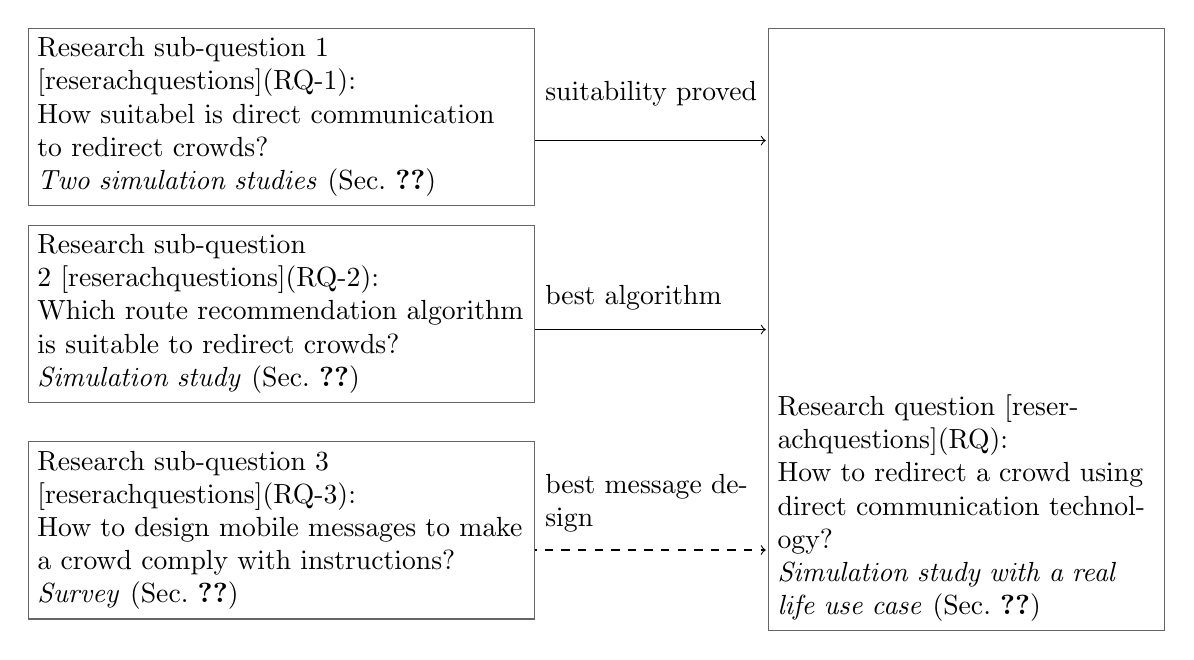
\begin{tikzpicture}
\draw [->] (3,-0.3) -- (6.65,-0.3);
\draw [->] (3,-2.7) -- (6.65,-2.7);
\draw [->, dashed] (3,-5.5) -- (6.65,-5.5);
\node[rectangle,draw=black!60,fill=white,text width=6.2cm] at (0.5,0.0)                            {{Research sub-question 1} ~\hyperref[reserachquestions]{(RQ-1)}: \\  How suitabel is direct communication to redirect crowds? \\ \textit{Two simulation studies}  (Sec.~\ref{sec:infoverbreitung})};
\node[rectangle,draw=black!60,fill=white,text width=6.2cm] at (0.5,-2.5)                            {{Research sub-question 2}~\hyperref[reserachquestions]{(RQ-2)}: \\ Which route recommendation algorithm is suitable to redirect crowds?\\ \textit{Simulation study}   (Sec.~\ref{sec:umleitalgorithmen})};
\node[rectangle,draw=black!60,fill=white,text width=6.2cm] at (0.5,-5.25)                            {{Research sub-question 3} ~\hyperref[reserachquestions]{(RQ-3)}: \\ How to design mobile messages to make a crowd comply with instructions? \\ \textit{Survey}  (Sec.~\ref{sec:reaction})};
\node[rectangle,draw=black!60,fill=white,text width=4.8cm, text height=4.8cm] at (9.2,-2.7)                            {Research question~\hyperref[reserachquestions]{(RQ)}: \\ How to redirect a crowd using direct communication technology? \\ \textit{Simulation study with a real life use case}  (Sec.~\ref{sec:realistiscscenario})};
%\draw [black,
    decorate, 
    decoration = {brace,
        raise=-15pt,
        amplitude=5pt}] (8,-4.5) --  (4,-4.5)
node[pos=0.5,black]{Assembling};
%\draw [->] (5,0) -- node [text width=2.5cm,midway,above ] {prerequisited} (8,0);
\node[text width=2.9cm] at (5.3,0.3){suitability proved};
\node[text width=2.9cm] at (5.3,-2.3){best algorithm};
\node[text width=2.9cm] at (5.3,-4.9){best message design};
\end{tikzpicture}
\caption[Structure of the chapter ]{Structure of the chapter. In the Sections~\ref{sec:infoverbreitung}-\ref{sec:reaction}, I answer  research sub-questions. My proposal of a crowd guidance system and a proof of concept can be found in  Section~\ref{sec:realistiscscenario}.}
\label{fig:reserachdesign}
\end{figure}





\section{Information dissemination in a mobile crowd}
\label{sec:infoverbreitung}

In this section, it is investigated how reliably route recommendations are disseminated through direct communication technologies in a mobile crowd (sub-question~\hyperref[reserachquestions]{RQ-1}). To answer the question, I design a worst-case scenario. If the information dissemination succeeds, I expect that it will be reliable in many real-life use cases.
The worst case is that interference and shadowing lead to a breakdown of the information dissemination. While interference might be controlled through protocols, shadowing is determined by the topography: Physical obstacles not only limit the line of sight but also hinder mobile communication. 

The crowd and the mobile network form a complex socio-technical system. If the crowd size is loose and crowd members may be isolated, shadowing affects the information dissemination and, thus, the crowd dynamics. In dense crowds, the effect of interference will be dominant. To better understand the system's dynamics I divide the study into two parts. The first part focuses on the effect of shadowing when the crowd is loose. The second part focuses on the reliability of the information dissemination process in a dense crowd when there are many crowd members to relay the information around obstacles. The questions to be answered are:

\begin{itemize}
\item Sub-study 1 (in the presence of shadowing): How many crowd members are necessary in the worst-case scenario that shadowing does not disturb the information dissemination?
\item Sub-study 2 (no impairment through shadowing): How fast is the information disseminated? What is the effect of uncertain simulation parameters?
\end{itemize}

The section is structured as follows: First, a worst-case research scenario is designed where the mobile communication in a crowd is blocked by obstacles. Then a criterion is proposed that evaluates the reliability of the information dissemination in a mobile crowd. In particular, I discuss why microscopic quantities of interest from the research field of mobile networks are not suitable for my investigations. Then, the model of the crowd guidance system is presented, where a crowd should receive static detour information about a closed gate. 
In both simulation studies, the same scenario, model and implementation is used. The difference between the studies is the set of analyzed parameters and the research methodology. At the end of the section, the results are summarized and discussed. Then, I evaluate what these findings implicate for the design of my crowd guidance system.


\subsection{Research scenario}

Imagine a complex building, such as a train station with multiple entrances and exits, where an entrance or exit is suddenly closed. 
Since walking routes are not directly visible due to walls or other obstacles, it is necessary to inform passengers about the detour. For this purpose, a mobile application based on direct communication technology should be used. When information is disseminated over the mobile network, pedestrians might be separated by obstacles (shadowing). Due to that, detour information  may not be disseminated successfully over the mobile network. To investigate this effect, I pose several requirements for the research scenario:


\begin{enumerate}
\item Pedestrians have a limited view: they cannot see the closure of the route directly. 
\item The information about the closure is distributed via a mobile application based on direct communication.
\item Communication between shadowed pedestrians is only possible via intermediate nodes or by them changing position, which resolves shadowing.
\item Only people who have personally seen the closure on site generate and send redirection information (there are no sensors that detect the closure automatically).
\end{enumerate}
The last point implicates extreme conditions: The closed gate is located in a niche so that pedestrians, who provide information, are completely shadowed from the area where the information is needed.
Hence, the conditions are more restrictive than in the scenario from my related publication~\cite{mayr-2021-com}, see Appendix~\ref{sec:effectofnetworktraffic}.


The topography is depicted in Fig.~\ref{fig:InfoDissSzenario}. It covers an area of $176\,\text{m}\,\times \,129\,\text{m}$. Crowd members at a train station take different routes to get to the train. Suddenly, the left path is closed, forcing pedestrians to take a different route.  The agents are generated from four sources at the north and walk along different routes to the destination at the south. The number of agents can be controlled through a source parameter. 
After $100\,\text{s}$, an agent next to the closed gate decides to inform others about the closure. It generates a route recommendation and sends it via a mobile application as a groupcast to all agents in the scenario. The technology used is direct communication based on the 802.11p WLAN standard. Agents that receive the detour information forward it.

%A more detailed description of how the mobile applications that are used to send and receive the rerouting information work can be found in the next section.
As soon as agents receive the rerouting information, they take the alternative route. This is based on the assumption that all people follow the route recommendations, which is optimistic. In this study, I will refrain from examining the pedestrians' compliance to follow route recommendations because it would be computationally too expensive, and I refer to Section~\ref{sec:umleitalgorithmen}, in which the effect of compliance is investigated.



% Mir ist bewusst, dass ich mit dieser Untersuchung keine generellen Aussagen über die Zuverlässigkeit von direkter Kommunikation treffen können. Hierfür gibt es zu viele Unbekannte: Wie sieht die Topografie aus? Welcher Mobilfunk-Technologie wird verwendet? Wie viele Personen besitzen ein Mobiltelefon, das zur direkten Kommunikation fähig ist?










\subsection{Reliability of information provision}

In the research field of mobile communication, there are several metrics and quantities for evaluating the performance of a network, such as latency or jitter. These quantities are microscopic and refer to individual packet transmissions which is important to look at when designing network technologies. However, these metrics do not consider the information state of the crowd as a whole. Therefore, they are not suitable for my investigations.

Moreover, mobile communication and crowd locomotion have different temporal and spatial scales. Packets in a mobile network are transmitted within a few milliseconds over hundreds of meters. The average pedestrian is much slower with a typical speed between $1\,m/s$ and $1.5\,m/s$. Also, pedestrians need time to process information. An information delay of a few milliseconds does not affect the locomotion of the crowd as a whole. 

I propose the following macroscopic quantities to evaluate the information process in a mobile crowd:
\begin{itemize}
\item \textit{Information degree} $p$: percentage of crowd members that have received detour information
\item \textit{Dissemination time} $t_{diss}$: time between the point of time when the route recommendation was sent the first time and the time when a certain proportion  $p$  of the crowd members has been informed. I propose $p_{threshold}=100\,$\% for closed system (no arrivals, no departures). For open systems where people continuously arrive or leave the scenario, I propose to choose $p_{threshold}\leq 100\,$\% depending on the arrival and departure rate. In the two sub-studies, $p_{threshold}=95\,$\% is used.
\end{itemize}



\begin{figure}[H]
\centering
\includegraphics[width=11cm,clip,trim={0.5cm 0 6.0cm 0}]{../figures/investigation/Informationsverbreitung/scenario.pdf} 
\caption[Worst case scenario for investigating information dissemination in a mobile crowd]{Worst case scenario for investigating information dissemination in a mobile crowd.  Representation of the scenario in \textit{Vadere} (top) and \textit{OMNeT++} (bottom). The size of the scenario is $176\,\text{m}\, \times \,129\,\text{m}$. The grid with $5\,\text{m}$ cell width provides orientation (bottom). The agents (blue and red circles) walk from the green source (top) to the target (bottom) on different routes. Agents marked red take a detour, since the left gate (brown area) is closed. The orange area is the area where the closure is in their line-of-sight, so that they start to detour. }
\label{fig:InfoDissSzenario}
\end{figure}




To evaluate the reliability of information dissemination, I propose the following criterion:
\begin{itemize}
\item The information dissemination is reliable if the \textit{dissemination time} $t_{diss}$ does not exceed the threshold value $t_{threshold}$: $t_{diss}\leq t_{threshold}$. Otherwise, if $t_{diss} > t_{threshold}$, information propagation is not reliable.
\end{itemize}
As threshold value I choose $t_{threshold}=10$\,s because within $10$\,s even running pedestrians ($3.0\,\text{m/s}$) receive the information within the arrival area (176\,m$\times$30\,m) where a change of the route choice would not increase the length of the walking path.

To check the plausibility of the simulation results, I compare the \textit{dissemination time} with the statistics of the microscopic quantity of interest \textit{packet lifetime}. The \textit{packet lifetime} describes how long the transmission of a packet takes. 
I expect that the maximum value of the \textit{packet lifetime} and the \textit{dissemination time} have the same order of magnitude. I do not expect that they are equal, since information is transmitted over intermediate nodes. If so, multiple packets are necessary, and, the time it takes to receive information becomes the sum of all \textit{packet lifetimes}. 





\subsection{Model and implementation of the crowd guidance system}

The simulation model of the crowd guidance system is composed of several component models, see Tab.~\ref{tab:composedmodelstudy1}. In the following, the component models are briefly introduced. It is explained why a certain model is chosen for the investigation and hot it is implemented in the \textit{CrowNet} simulator.

\begin{table}[hbt!]
\begin{footnotesize}
\begin{tabular}{|p{2cm}|p{2.6cm}p{3.2cm}p{5cm}|}
\hline
\textbf{Component} & \textbf{Sub-component} & \textbf{Model}  & \textbf{Implementation (Simulator)} \\ \hline
Crowd  & Locomotion model & Optimal Steps Model & OptimalStepsModel (Vadere) \\ \cline{2-4}
& Perception model &  Assumption: info is always perceived & impl. in UdpDetourApp (CrowNet)  \\ \cline{2-4}
& Cognition model & Assumption: 100\% compliance & UdpDetourApp (CrowNet/app.)  \\ \hline

Controller &
Time stepping alg. & Fixed interval (default: 1s) & UdpDetourApp (CrowNet/app.)  \\ \cline{2-4}
&  Route recommendation alg. & None (static information: Gate closed) & Not needed \\ \hline

Network & Application layer & Detour application &  UdpDetourApp  (CrowNet/app.) \\ \cline{3-4}
&& Receive and forward information &  UdpDetourAppVadere  (CrowNet/app.) \\ \cline{2-4}
&Transport layer & Udp  & {Udp} (inet) \\ \cline{2-4}
&Network layer & Ipv4  &{Ipv4NetworkConfigurator} (inet) \\ \cline{2-4}
&Data Link layer & acc. IEEE 802.11 & {Ieee80211MgmtAdhoc} (inet)   \\ \cline{2-4}
&Physical layer &  & \\  
&$\rightarrow$ Channel model & acc. IEEE 802.11 & {Ieee80211DimensionalRadio} and Ieee80211DimensionalRadioMedium (inet) \\ 
&$\rightarrow$ Obstacle Model & Ideal Obstacle model & IdealObstacleLoss (inet)  \\ 

\hline
\end{tabular} 
\end{footnotesize}
\caption[Component models for investigating information dissemination in a crowd]{Component  models for investigating information dissemination in a crowd. If not specified, I use parameter values and settings for the component models. The mobile network model is composed of the protocol stack and the channel model. Importantly, the ideal obstacle model is used to model transmission failures due to shadowing: The transmission fails if agents are not in line-of-sight.}
\label{tab:composedmodelstudy1}
\end{table}




\subsubsection{Crowd behavior}
I assume that all people follow the recommendation to take the alternative route immediately. This assumption may be optimistic, but it should not affect the macroscopic quantities of interest: Even if only a part of the crowd followed the route recommendation, the left stream in Fig.~\ref{fig:InfoDissSzenario} would become wider because non-compliant agents continue to walk downwards while compliant agents turn right.
Nevertheless, the agents form a connected graph within the arrival area. As a consequence, the topology of the network would be similar.  The transmission of individual packets might change, but this should not affect the macroscopic \textit{dissemination time}.
 

After receiving detour information, the target of agent is directly changed without modeling the perception or cognition. The targets are set in the \lstinline{UdpDetourApp} (\textit{OMNeT++}) when an agent receives the information over the mobile network, see Tab.~\ref{tab:composedmodelstudy1}. The \lstinline{UdpDetourApp} then triggers the target change in \textit{Vadere} via the Traffic Control Interface (TraCI). 
To model the locomotion behavior, the Optimal Steps Model is used that is implemented in the  \textit{Vadere} simulator.



\subsubsection{Route recommendation generation}
In the scenario, there is no need for a sophisticated route recommendation algorithm because there is only one route left: This route is recommended all the time. Thus, there is no need to integrate the \textit{flowcontrol} simulator. Instead, a simple redirection model is implemented in the \lstinline{UdpDetourApp} application of the \textit{OMNeT++} module, see Fig.~\ref{fig:study1Simulatorsinvolved}. The redirection model sends static information (`The left gate is closed. Please use the right gate').


\begin{figure}[hbt!]
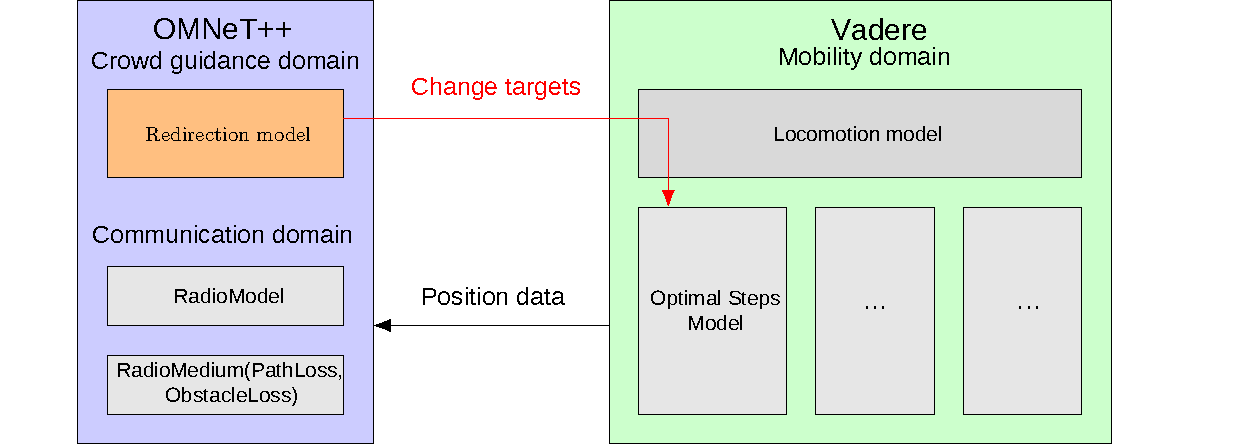
\includegraphics[width=\textwidth,trim={0.2cm 0 1cm 0cm}]{figures/investigation/Informationsverbreitung/ModelInteraction.pdf}  
\caption[Simulation approach in the information dissemination study]{Simulation approach in the information dissemination study. The simulators \textit{OMNeT++} and \textit{Vadere} communicate over the Traffic Control Interface. When detour information has been received in the mobile networks simulation (left), the targets are changed in the crowd simulation (right). Agents' positions from the crowd simulation are shared at the simulation time step of the \textit{Vadere} simulator (0.4s). Image as in my publication~\cite{mayr-2021-com}. }
\label{fig:study1Simulatorsinvolved}
\end{figure}




\subsubsection{Information dissemination through direct communication}

In my investigations I want to test the worst case. Therefore, I suggest to use direct communication according to the IEEE 802.11p standard. If one can inform a mobile crowd based on this technology, it is likely that more advanced technologies based on IEEE 802.11bd or cellular communication may also be suitable. 
Therefore, models for the 802.11p standard are selected on the link and physical layer. The link layer model   handles the sending and reception process of data frames that are passed from device to device. There are no control or management frames. As implementation the module \textit{Ieee80211MgmtAdhoc} from the \textit{INET} framework is used.

The signal modeling is specified at the physical layer. 
To model the signal power in the analog domain, a models are used that describes the change of the signal power over time and frequency: 
 the \textit{Ieee80211DimensionalRadio} model in conjunction with the \textit{Ieee80211DimensionalRadioMedium} model from the \textit{INET} library.

To capture the signal attenuation caused by obstacles, I choose the Ideal Obstacle Model to model the worst case:  If there is an obstacle in line-of-sight, there is no signal strength at all. In a real-life use case, the signal would be attenuated. Therefore, I believe that information dissemination is successful in real life, when it is successful in the simulation because conditions are milder. Using the Ideal Obstacle Model has another advantage: No permeability of the obstacles needs to be defined which keeps the dimensionality of the parameter space low. As implementation the \textit{IdealObstacleModel} from \textit{INET} is used.
 

The sending of the route recommendation is modeled as a mobile application on the application layer. When the application is started, it sends the redirection recommendation at fixed time intervals. Packets are broadcasted via a link local broadcast. No routing protocol is used. The application is implemented as a finite-state machine in the \textit{OMNeT++} module of the \textit{CrowNet} simulator, see Fig.~\ref{sec:controllermodel}. Note that in the scenario only one agent next to the closed gate sends route recommendations. Other agents only receive and forward the information.

Every agent has an application assigned that receives and forwards detour information. The application manages the change of the targets over the Traffic Control Interface. As soon as the detour information is received, the destination contained in the route recommendation is set for the agent. Then, the packet is forwarded via broadcast. An internal timer ensures that the route recommendation is only processed once. This helps to avoid a broadcast storm. As implementation, the \textit{UdpDetourAppVadere} application is implemented in the \textit{OMNeT++} module.



\begin{figure}[hbt!]
\centering
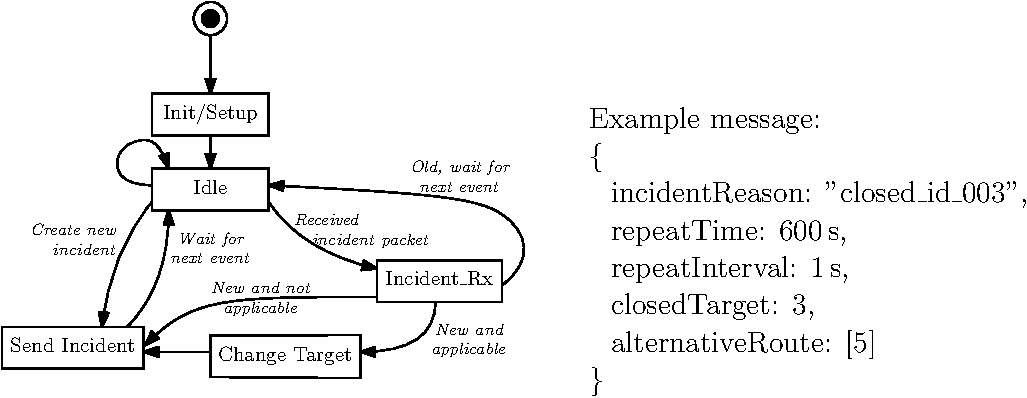
\includegraphics[width=0.9\textwidth]{figures/investigation/Informationsverbreitung/ControlModel.pdf} 
\caption[Controller model generating and forwarding detour information]{Controller model generating and forwarding detour information. Since the left gate (target id=3) is closed, agents are redirected to the right gate (target id=5). The information is provided in time intervals of $1\,s$. 
Image as in my publication~\cite{mayr-2021-com}.}
\label{sec:controllermodel}
\end{figure}





\subsection{Minimal crowd size to avoid shadowing}

In the first sub-study, I want to find out the minimum number of crowd members necessary in my scenario to ensure that the dissemination of route recommendation does not fail due to shadowing. I use the minimum number in the next sub-study as lower bound for an uncertain parameter when conducting an uncertainty quantification study.


\subsubsection{Methodology: varying the crowd size}
To find out how many crowd members are needed to avoid shadowing, the parameter \textit{number of agents} is varied between 20 and 150.  I choose a lower bound of 20 agents due to the following consideration. To prevent shadowing, at least 8 nodes (2$\times$4) are needed: four agents around the wall (W1) and four agents around the room (R1), see Fig.~\ref{fig:InfoDissSzenario}. Another node is required to transport the information to the target area. Since agents' positions are continuously changing, I choose 20 nodes to be on the safe side. I choose an upper bound of 150 agents because one can assume that agents form a connected chain which prevents the effect of shadowing. In total, 500 samples are generated which requires to run the simulation 500 times. 

Since the number of agents is still low, it is likely that the information distribution fails due to shadowing rather than interference. Therefore, I assume, that shadowing is present when the information dissemination fails, that is, when less than $95\,$\% of the agents are informed after $10\,\text{s}$: $p=0.95, t_{threshold}=10\,\text{s}$.  
%I choose discrete parameter values: 20.00, 20.26, 20.52, ... , 149.74, 150.00. Please note that there are of course no half or quarter agents: the number of agents is will be rounded. The decimal place only changes random objects in the simulation. This allows me to take into account the stochastic behavior of pedestrian flows without having to generate different seeds.
%Die ist aus meiner Sicht in dieser Untersuchung notwendig, da die Abschattung zufällig durch die Agentenpositionen entsteht. Die Positionen hängen dabei wiederum von den Laufgeschwindigkeiten der Agenten ab. Da diese aus einer Zufallsverteilung gezogen werden, gehe ich davon aus, dass 

%Bei einer Änderung des seeds laufen die Personen mit anderen Laufgeschwindigkeiten, wodurch sie neue Positionen einnehmen, was Abschattung auflösen oder begünstigen kann. 


\subsubsection{The information dissemination fails due to shadowing}
To ensure that shadowing causes the dissemination failure I randomly select samples with $t_{dissemination}>10\,\text{s}$. I observe that the crowd is indeed temporarily separated by obstacles during the information dissemination process (simulation time $\in [100\,\text{s}, 110\,\text{s}]$), see Fig.~\ref{fig:shadowingexample}. One can observe three separated crowds: A crowd on the left, a crowd on the right and a crowd at the bottom, each represented by blue connecting lines between them. The left crowd is in line-of-sight with the crowd on the right which allows them to pass on information. However, the crowd at the bottom is still shadowed by a wall, so that the four agents close to the target are not informed within $10\,\text{s}$. As a result, the information degree is only  81\,\% after 10\,s (17 of 21 agents have been informed). The visual check strongly indicates that the information dissemination indeed fails due to shadowing when the parameter \textit{number of agents} has a low value.  

\begin{figure}[hbt!]

\begin{tikzpicture}
\node[] at (0,0) {\includegraphics[height=5cm]{./investigation/Informationsverbreitung/Sample_0_shadowing_study/shadowing_sample_0_0.pdf} 
};
\node[] at (8,0.6) {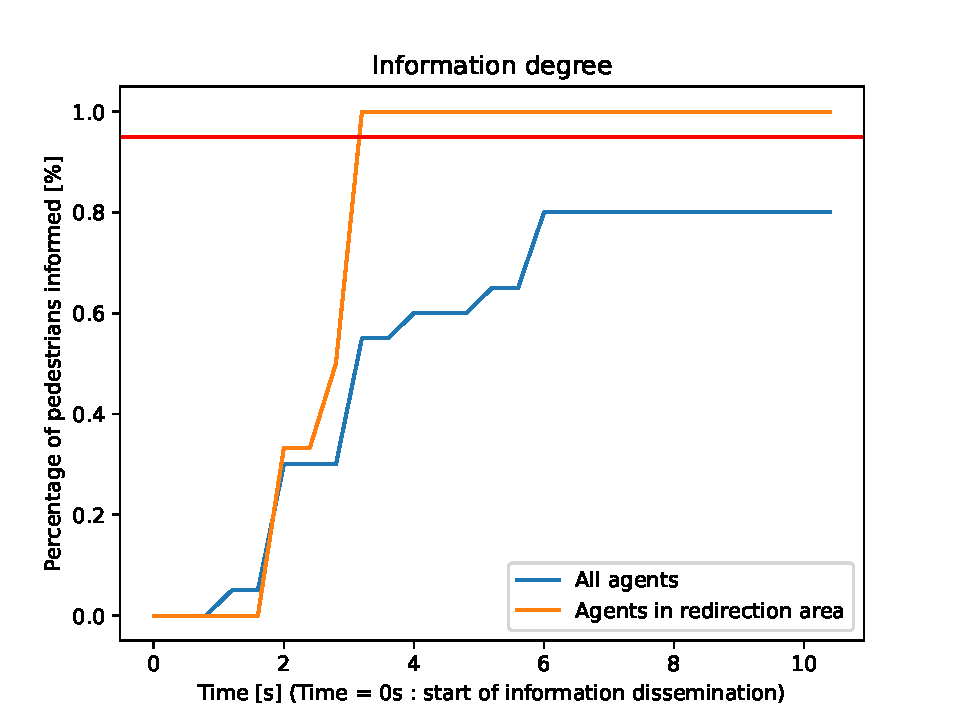
\includegraphics[height=5cm,trim={1.1cm 0.8cm 0cm 0cm},clip]{./investigation/Informationsverbreitung/Sample_0_shadowing_study/InformationDegree.pdf}
};
\node[font=\small, fill=white, text width=7.5cm,align=center] at (7.8,-2.5)  {Time in s  \\ (after info. dissemination started)};
\node[font=\small, fill=white, text width=5.5cm,rotate=90, align=center] at (4.25,0.0)  {Proportion of informed agents in \%};
\draw[color=orange,dashed] (-3.65,0.8) rectangle (3.65,2.45);
\node[font=\tiny,color=orange] at (-2.1,1.9)  {Redirection area (dashed)};
\node[font=\tiny, text width=2cm] at (-1.4,-1.6)  {Information source};
\end{tikzpicture}
\caption[Partially informed crowd due to shadowing]{Partially informed crowd due to shadowing. The crowd is separated by obstacles (see red lines through obstacles on the left). As a consequence, only 17 out of 21 (81\,\%) agents in total are informed after 10\,s (right). Agents in the arrival area have been informed successfully after 3.2\,s (intersection of the orange line and the red threshold line on the right) because agents form a chain in this area (see blue lines connected to the information source on the left). }
\label{fig:shadowingexample}
\end{figure}
 




\subsubsection{Probability for shadowing in dependency of the crowd size}

To determine the probability for shadowing in the scenario, the values of the parameter \textit{number of agents} are grouped into bins. For each bin, it is counted how often shadowing was present. To obtain the probability the count is normalized by the total number of samples. The result is depicted in Fig.~\ref{fig:shadowing}. 

\begin{figure}[hbt!]
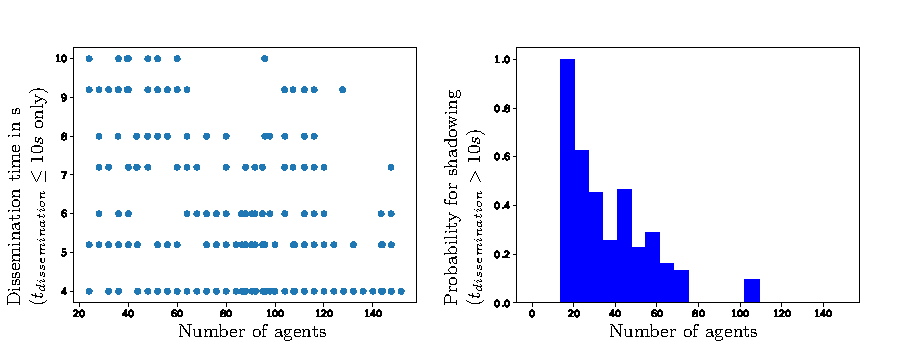
\includegraphics[width=\textwidth]{../figures/investigation/crownetOutput/shadowing/ProbabilityforShadowingCrowdSize.pdf} 
\caption[Information dissemination time and probability for shadowing]{Information dissemination time and probability for shadowing. The information dissemination is successful when the dissemination time is $\leq10\,\text{s}$ (left).  Note that the information dissemination time is a multiple of the time step size $0.4\,\text{s}$. The more agents, the less likely shadowing is (right). In the research scenario, shadowing is no longer present when the crowd has more than 110 members. }
\label{fig:shadowing}
\end{figure}


As expected, the probability of shadowing decreases over the uncertain parameter \textit{number of agents}. In the scenario, there appears to be no more shadowing with more than 110 agents. Below this threshold, shadowing is likely to occur. However, one cannot predict whether shadowing occurs for a specific sample, since the crowd locomotion is stochastic: Agents' walking speeds are randomly drawn from a normal distribution. A change of the seed or a slightly different value of a parameter changes agents positions. One can observe that communication can even succeed if the \textit{number of agents} is small: For 30 agents only, the \textit{dissemination time} is less than $5.2\,\text{s}$, see Fig.~\ref{fig:shadowing} (left). However, this is a stochastic effect that cannot be controlled.



\subsubsection{Summary of the shadowing study: shadowing is prevented with a sufficient dense crowd}
The first sub-study suggests that with enough well distributed agents present, loss of information through shadowing can be completely avoided. In the scenario 110 agents sufficed to spread detour information in a crowd in less than 10 seconds. I conclude this is enough time to inform agents about a closure before they take a closed route.



\subsection{Effect of uncertainties on the information dissemination}

\subsubsection{Motivation for quantifying uncertainties}
%We know from the previous study that information distribution using direct communication can fail when crowd sizes are small. In this sub-study, I will assess how reliably information is disseminated in the absence of shadowing. 


The crowd size in real-life scenarios, like at a train station or a festival, is often uncertain. Apart from the crowd size, there are additional unknowns, such as the transmitter power of smartphones. I aim to understand how such uncertainties impact the reliability of the information dissemination. 
Therefore, uncertainty quantification methods are applied. I choose a surrogate-based approach with polynomial chaos expansions to reduce the computational effort because a single simulation run can take several hours.

Forward propagation is employed to assess the effect of uncertain parameters on the quantities of interest. A global sensitivity study is conducted to quantify the influence of parameters.

The sub-study is structured as follows. First, the set of parameters and quantities of interest is introduced. Second, the simulation pipeline is described which comprises the construction of the polynomial chaos expansions. Finally, the results are discussed. I expect the reader to be familiar with the theory on polynomial chaos expansions, forward propagation and global sensitivity analysis (see Section~\ref{sec:uq}).


\subsubsection{Parameter selection for the uncertainty quantification}
I consider two uncertain parameters that I think are particularly interesting for a crowd guidance system: the \textit{number of agents} and the \textit{transmission interval}, see Tab.~\ref{tab:parameterstudy1}. The parameter \textit{transmitter power} only serves as a control. 

\begin{table}[hbt!]
\centering
\begin{tabular}{@{}llrrl@{}}%
\toprule
Parameter                        & Unit & Distribution & Sample points                                  \\ \midrule
Number of agents $n$ & 1    & U(200,2500) & 415, 1325, 2235    \\
Transmitter power $p$      & mW   & U(2.0, 20.0) & 4.03,11.00, 17.97     \\
Transmission interval $si$        & s   & U(0.8,2.8)   & 1.0, 1.8, 2.6       \\
\bottomrule
\end{tabular}%
\\ \vspace{0.3cm}
\caption[Uncertain parameters in the information dissemination study]{Uncertain parameters in the information dissemination study. The three parameters are used in the forward propagation and in the global sensitivity analysis. Since the shape of the distributions are unknown, I use uniform distributions.   Three sample points for each parameter are needed to construct a polynomial chaos expansion of order\,$=2$. In total, there are $27\,(=3^3)$ samples.   }%
\label{tab:parameterstudy1}%
\end{table}%

The first parameter is the \textit{number of agents}. The previous part of the study demonstrated how communication fails due to shadowing when the \textit{number of agents} is low. A high \textit{number of agents} can, in turn, lead to interference in the mobile network or congestion in passenger traffic. Thus, this parameter controls the dynamics of  the complex socio-technical system composed of the crowd and the mobile network. Since I do not know the distribution type of the parameter, I use a unit distribution. As lower bound I use a \textit{number of agents} of 200 (the previous study required at least  110 to prevent shadowing). As upper limit I choose 2500.  More agents would lead to a congestion where agents do no longer move at all. I want to avoid a change of the crowd dynamics because this opens the question whether changes in the information dissemination process are caused by a change of the crowd dynamics or by a change of the mobile network.  

The second parameter is the \textit{transmission interval}. At the simulation time 100\,s, one agent next to the closed gate (see Fig.~\ref{fig:InfoDissSzenario}) starts to send detour information repeatedly over broadcast.   The \textit{transmission interval} is the time in between two broadcast rounds. The repetitions increase the probability that information is successfully disseminated even if the communication locally or temporarily breaks due to interference. However, the smaller the transmission interval, the higher the risk for collisions and interference. Therefore, I choose a lower bound of 0.8\,s. As upper bound I choose 2.8\,s which means that the broadcast is re-started four times within 10\,s: 0\,s, 2.8\,s, 5.6\,s, 7.8\,s. I argue four chances should be enough to disseminate information. 


The third parameter is the \textit{transmitter power} of the smart phone's antennas. In combination with  other parameters such as the receiver sensitivity of the antennas, this parameter determines the range for communication. It serves as a control because this parameter does not have an effect: The scenario is sufficiently small so that agents are always in communication range (see Appendix~\ref{sec:networkparameters}). I choose a parameter range [2.0\,mW, 20.0\,mW] which is typical for many types of smartphones.  % I assume default values for all other parameters that influence the range.

\subsubsection{Selection of quantities of interest}

I am interested in six scalar quantities of interest:
\begin{itemize}
\item \textit{TimeAll}: Dissemination time ($p=0.95$) referring to all agents: How long does it take until 95\,\% of the agents are informed about the detour? Accuracy: time step size 0.4\,s. \textit{SI-Unit: s}
\item \textit{TimeArrArea}: Dissemination time ($p=0.95$) referring to agents in the arrival area: How long does it take until 95\% of the agents are informed in the arrival area? Accuracy: time step size 0.4\,s. \textit{SI-Unit: s}
\item \textit{NumAgents}: I use the number of agents as control (similar to the control parameter transmitter power; here the number of agents is a measurement quantity not a parameter). \textit{SI-Unit: 1}
\end{itemize}
Please note that the \textit{dissemination times} are always a multiple of the simulation step size of the \textit{Vader}e simulator (0.4\,s). 

The information is successfully disseminated when at least $p=95$\% of the agents have been informed. A proportion of $p=95$\% ensures that the information degree is not underestimated due to short-term fluctuations caused by informed agents that reach the target or leave the reference area.

To check the plausibility of the simulation results, I compare the \textit{dissemination time} with the statistics of the microscopic quantity of interest \textit{packet lifetime}. The  \textit{packet lifetime} describes how long it takes that a packet is transmitted in the mobile network from a sender to a receiver.  %If the route recommendation fits into a packet and if the transmission takes place without intermediate nodes, 

\begin{itemize}
\item \textit{MaxPackLifetime}: maximal packet lifetime. \textit{SI-Unit: s}
\item \textit{MedPackLifetime}: median packet lifetime. \textit{SI-Unit: s}
\item \textit{MinPackLifetime}: minimal packet lifetime. \textit{SI-Unit: s}
\end{itemize}

I expect that the \textit{maximal packet lifetime} and the \textit{dissemination times} have the same magnitude. I further expect that the \textit{maximal packet lifetime} is higher than the information dissemination time since the \textit{dissemination time} refers to the 95\,\% of the agents who get informed first. I check both expectations when analyzing the results.



\subsubsection{Methodology: forward propagation and sensitivity analysis using polynomial chaos expansions}
I use polynomial chaos expansions for forward propagation and global sensitivity analysis. In total, I construct 6 polynomial chaos expansions: one for each quantity of interest, see Fig.~\ref{fig:uqmethodologystudy1}. The same order is chosen for all polynomial chaos expansions. Therefore, the same sampling can be used for their construction.
For the polynomial degree, I choose a quadratic approach (order\,=\,2) to capture linear and quadratic behaviors of the quantities of interest in dependency of the uncertain parameters. To model plateaus or rapid changes, higher orders would be necessary. However, I cannot further increase the order since the number of samples grows exponentially and running one simulation can take several hours.  To construct a polynomial chaos expansion of order 2, three grid points are required for each parameter. The grid point values can be found in Tab.~\ref{tab:parameterstudy1}. In total, this makes 27 samples or simulation runs. 

\begin{figure}[hbt!]
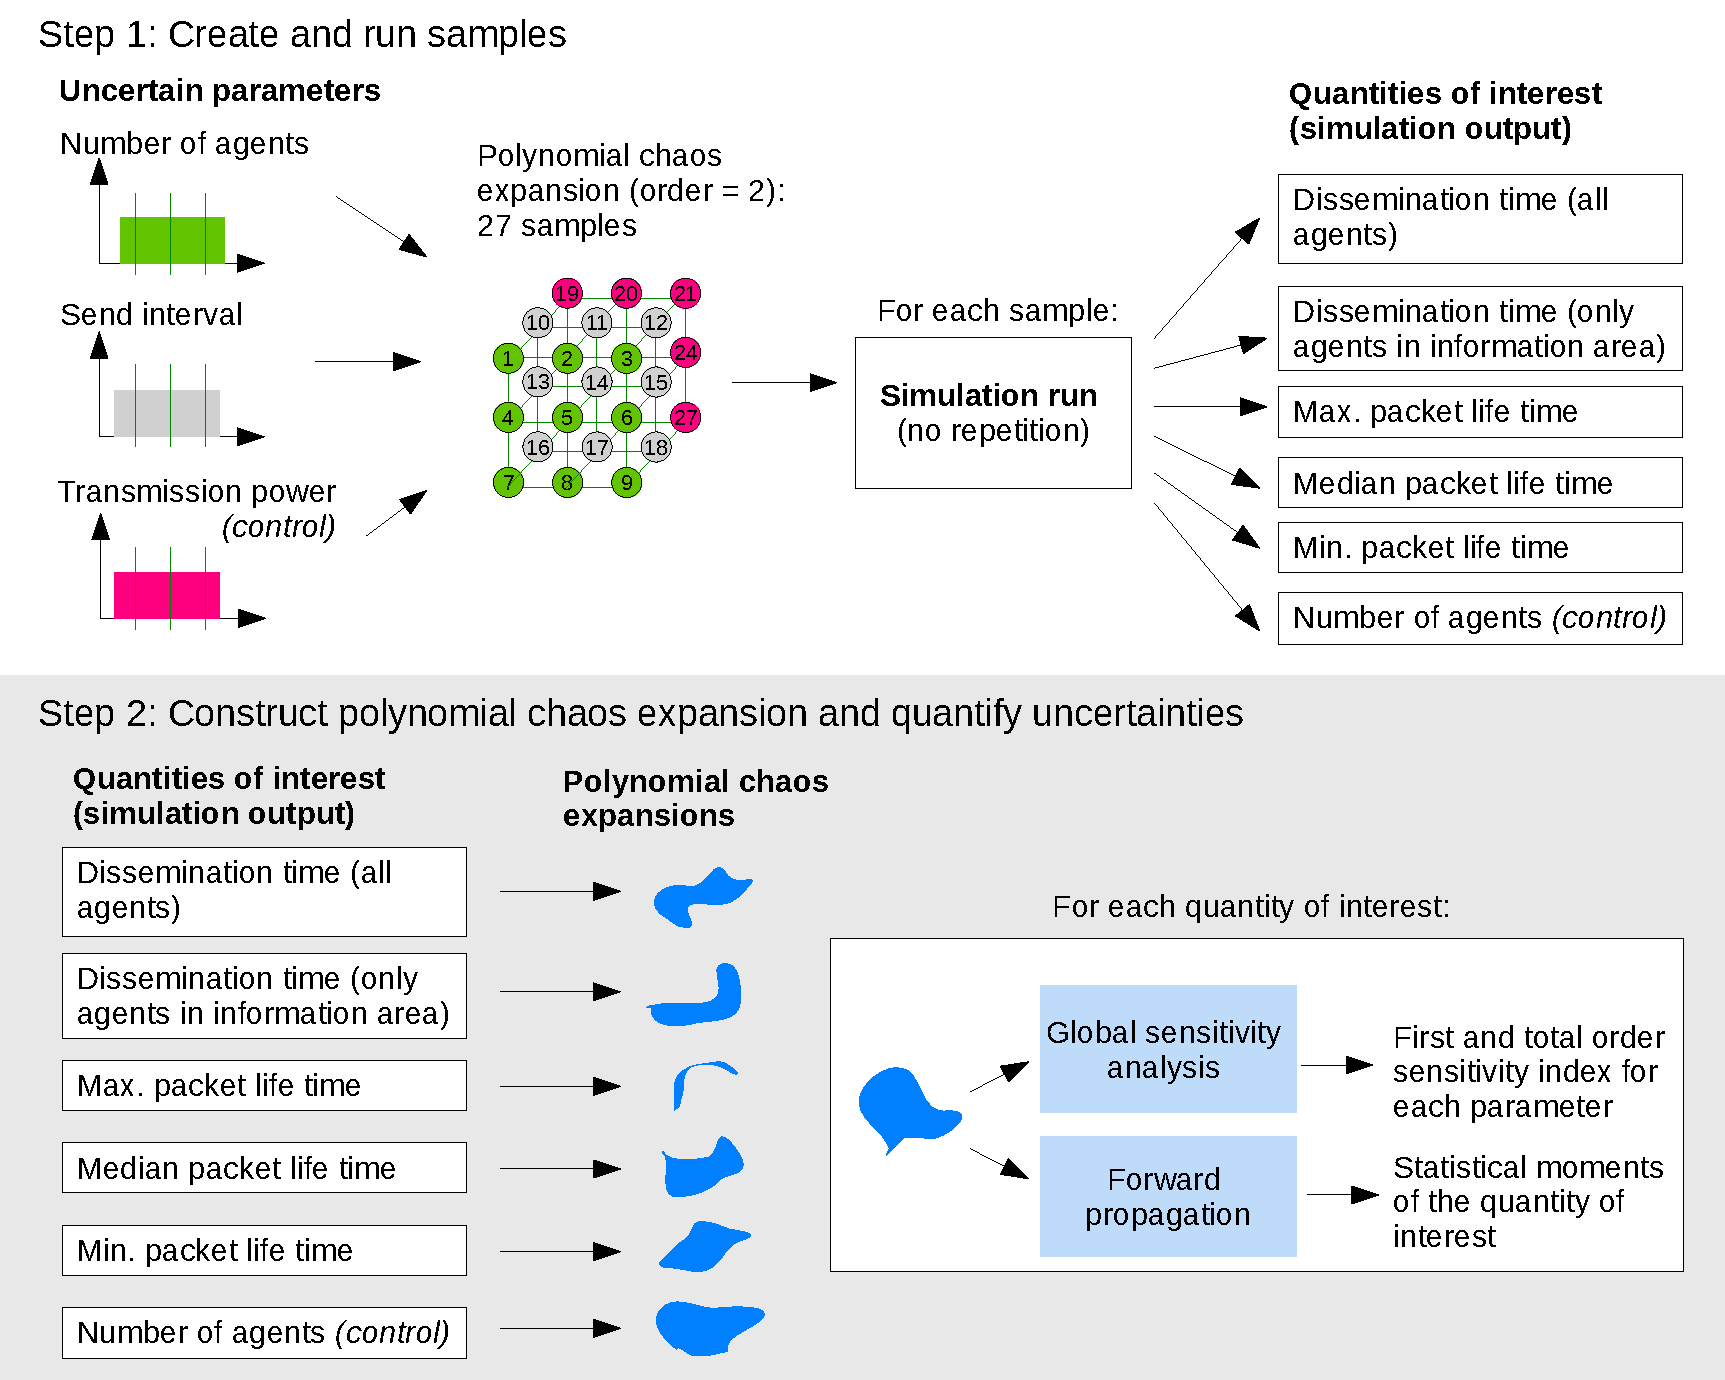
\includegraphics[width=\textwidth]{./investigation/Informationsverbreitung/uqprocedure.pdf} 
\caption[Parameters and quantities of interest for the forward propagation and sensitivity analysis]{Parameters and quantities of interest for forward propagation and global sensitivity analysis. I use polynomial chaos expansions for forward propagation and  sensitivity analysis. For each of the six quantities of interest, a polynomial chaos expansion of order 2 is constructed. With three parameters, 27 samples must be executed. From the expansions the first and total order sensitivity indices of the parameters and the statistical moments of the quantities of interest are computed. }
\label{fig:uqmethodologystudy1}
\end{figure}


Due to the long simulation duration of up to four hours, I do not carry out any repetitions, although random effects are present in my system. I argue that the influence of random effects is negligible 
because due to the \textit{number of agents} in the system the crowd forms a coherent communication network. I expect that there are local changes in the communication due to stochasticity. For example in one case agent (1) communicates directly with agent~(2) and agent~(3). In another case, agent~(1) communicates with agent~(2)~who passes the information on to agent~(3). As long as the network is coherent, I claim that such local effects have a negligible effect on the macroscopic \textit{dissemination times} or the statistical moments of the \textit{packet lifetime}. In fact, a preliminary study with one sample demonstrated that the quantities of interest do not differ qualitatively for the three tested seeds. This supports my claim, without being a general proof.

The simulation study is carried out with the \textit{SUQ-controller} module of \textit{CrowNet}. To reduce the total simulation time, 8 simulations are run in parallel using the virtual machine that is described in Appendix~\ref{sec:VirtualMachine}.





\subsubsection{Verification of the polynomial chaos expansions and plausibility check}
 
First, the correct construction of the polynomial chaos expansions is verified. The first control hypothesis is that the parameter \textit{transmitter power} has no influence. Tab.~\ref{tab:indicessensit} shows that this is indeed the case. Both the first and the total sensitivity index are zero, indicating that the parameter has no influence. 
The second control hypothesis is that the quantity of interest \textit{number of agents} depends only on the uncertain parameter \textit{number of agents}. This is indeed the case: Tab.~\ref{tab:indicessensit} shows that the first and total index of the parameter \textit{number of agents} is 1.0. All other indices are zero (see line \textit{NumAgents} in Tab.~\ref{tab:indicessensit}), which means that the other parameters have no influence. 
%With this in mind, I consider the construction of my polynomial chaos expansions as verified. I will not examine the control quantities "transmitter power" any further in the following.

Second, the simulation results are checked for plausibility. Tab.~\ref{tab:qoimoments} depicts the statistical moments of the quantities of interest. One can observe that the expected values of the \textit{median packet lifetime} (5.046\,s) and the \textit{dissemination time} (5.0\,s ... 5.4\,s) are equal for an accuracy of 0.4\,s. Importantly, they have the same order of magnitude. Therefore, the simulation results are plausible.

\begin{table}[hbt!]

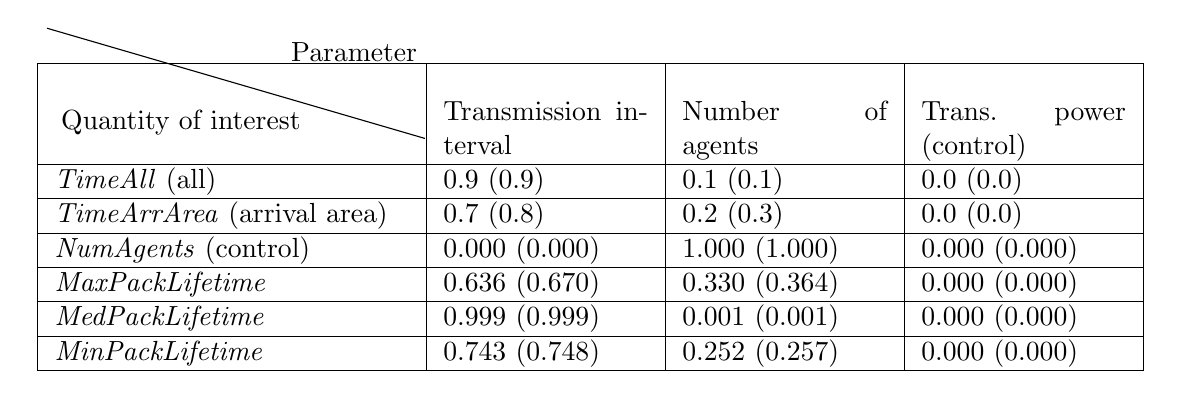
\begin{tikzpicture}

\node[] at (0,0) {
    \begin{tabular}{|p{4.5cm}|p{2.6cm}|p{2.6cm}|p{2.6cm}|}
    \hline
     & && \\
         &Transmission interval & Number of agents & Trans. power (control)  \\ \hline
       \textit{TimeAll} (all) & 0.9 (0.9) & 0.1 (0.1) & 0.0 (0.0) \\ \hline
        \textit{TimeArrArea} (arrival area) & 0.7 (0.8) & 0.2 (0.3) & 0.0 (0.0) \\ \hline
         \textit{NumAgents} (control)  & 0.000 (0.000) & 1.000 (1.000) & 0.000 (0.000) \\ \hline
         \textit{MaxPackLifetime} & 0.636 (0.670) & 0.330 (0.364) & 0.000 (0.000) \\ \hline
        \textit{MedPackLifetime}  & 0.999 (0.999) & 0.001 (0.001) & 0.000 (0.000) \\ \hline
       \textit{MinPackLifetime}  & 0.743 (0.748) & 0.252 (0.257) & 0.000 (0.000) \\ \hline
    
 \end{tabular}
 
 };
 \draw[] (-6.9,2.4) -- (-2.1,1);
  \node[] at (-5.2,1.2) {   Quantity of interest   };
    \node[] at (-3,2.1) {   Parameter    };

\end{tikzpicture}
 
\caption[First and total order sensitivity indices for the quantities of interest]{First and total order sensitivity indices for the quantities of interest. The indices are estimated using polynomial chaos expansions. The total effect indices are in brackets. As expected, the control parameter \textit{transmitter power} does not have any influence (indices: 0.0). The quantity of interest \textit{NumAgents} serves as a control: It only depends on the uncertain parameter \textit{number of agents}.  }
\label{tab:indicessensit}
\end{table}




%For the redirection of pedestrians, the information dissemination time in the redirection area is important. I expect that most of the people will decide on a route in this area and then stick to the route which makes them take a detour when they have not been informed successfully. This is why I look at the dissemination time referring to the redirection area. Tab.~\ref{tab:qoimoments}, one can expect that it takes about 3.2s ... 3.6s to inform the crowd in the redirection area. This might be slow at a scale of mobile networks communication, but it is fast at a scale of crowd locomotion: even fast pedestrians (2.2m/s) walk 8m far in 3.6s. I would expect that they have not already entered a route in many real life scenarios such as a train station. Depending on the parameters number of agents and sending interval, it can also take longer: the standard deviation is not zero (0.8s). However, as we have seen, this mostly depends on the choice of the sending interval which we are in control of. 

\begin{table}[hbt!]
\centering
\begin{footnotesize}


    \centering
    \begin{tabular}{p{3.3cm}p{2.5cm}p{2.3cm}p{2.8cm}}
    \hline
        Quantity of interest & ~ & Expected value & Standard deviation \\ \hline
       Dissemination time in s & \textit{TimeAll} & [5.0 ... 5.4[ & 1.2 %... 1.2 (=$\sqrt{1.2^2 + (0.4/2)^2}$) %/ 
       \\
        ~ & \textit{TimeArrArea} & [3.2 ... 3.6[ & 0.8 % ... 0.8 (=$\sqrt{0.8^2 + (0.4/2)^2}$)  
        \\ 
         Packet lifetime in s & \textit{MaxPackLifetime} & 7.548 & 0.730 \\ 
        ~ & \textit{MedPackLifetime} & 5.046 & 0.545 \\ 
        ~ & \textit{MinPackLifetime} & 4.973 & 0.701   \\ \hline
    \end{tabular}
    \end{footnotesize}
    \caption[Statistical moments for the quantities of interest]{Statistical moments for the quantities of interest. The statistical moments are estimates, derived from polynomial chaos expansions. 
    As the \textit{information degree} is only measured every 0.4\,s in \textit{Vadere}, the \textit{dissemination time} can only be specified with an accuracy of 0.4\,s. Accordingly, I use 1 decimal place only and provide  ranges for the expected values and standard deviations for the \textit{dissemination times}. Note that the range limits of the standard deviations differ in the second digit only under the assumption that the error of the standard deviation is 0.4\,s. }
\label{tab:qoimoments}
\end{table}




\subsubsection{Influence of the parameters \textit{number of agents} and \textit{transmission interval}}
Next the influence of the two parameters \textit{number of agents} and \textit{transmission interval} is analyzed. Tab~\ref{tab:indicessensit} shows their sensitivity indices for each quantity of interest. One observes that the first and the total sensitivity index (shown in brackets) are similar. This indicates that there are negligible interaction effects (second order effects) between the parameters. Thus, I use the first sensitivity index from now on.


The parameter \textit{number of agents} has only little influence on the information dissemination: For the \textit{median packet lifetime}, the sensitivity index is almost zero. This indicates no effect at all. For the \textit{minimum} and \textit{maximum packet lifetime}, the indices are low with 0.252 and 0.330 respectively. In fact the true values might be even lower because the indices also encounter variance caused by the varying sample size. The more agents, the more packet transmissions, and the more, accurately the bounds of the \textit{packet lifetime} distribution are captured. For the evaluation of the dissemination process, I, therefore, look at \textit{dissemination times} that are independent of the sample size.

The dissemination of information referring to all agents seems only slightly influenced (\textit{TimeAll} index: 0.1) by the \textit{number of agents}, see Tab.~\ref{tab:indicessensit}.
For agents in the arrival area, the influence is higher but still low (\textit{TimeArrArea} index: 0.2). The low influence can be verified visually in Fig.~\ref{fig:infodissplotdep}. For each \textit{transmission interval}, the \textit{dissemination time} is plotted over the \textit{number of agents}. The  data points correspond to the samples used for the polynomial chaos expansion. One can observe that the \textit{dissemination time} hardly changes over the \textit{number of agents} (left). For the arrival area (right), the \textit{dissemination time} changes over the \textit{number of agents} for certain \textit{transmission intervals}. I attribute this to the fact that fewer agents are in the arrival area than in the entire topography. Therefore, the local transmission of packets has a stronger influence on the \textit{dissemination time}. 
\begin{figure}[hbt!]
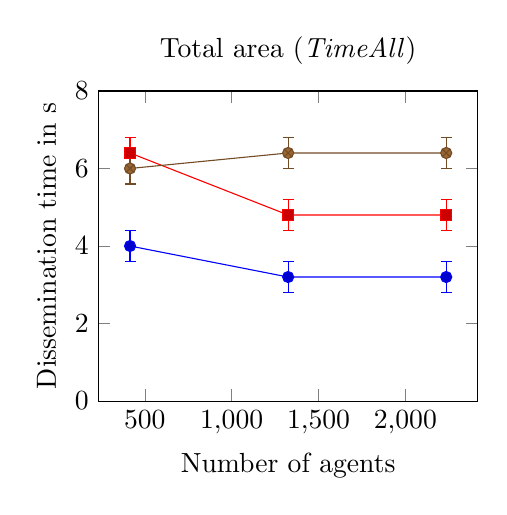
\begin{tikzpicture}
\begin{axis}[xlabel=Number of agents,ylabel=Dissemination time in s,title=Total area (\textit{TimeAll}), ymax=8,ymin=0,width=6.4cm]
\addplot+ [error bars/.cd,y dir=both,y fixed=0.4,
] table [x=Number,y=All,meta=Time] {
Time Number	All	Area
1.0	415	4.0	3.2
1.0	1325 3.2 3.2
1.0	2235 3.2 2.0
};
\addplot+ [error bars/.cd,y dir=both,y fixed=0.4,
] table [x=Number,y=All,meta=Time] {
Time Number	All	Area
1.8	415	6.4	2.8
1.8	1325 4.8 2.8
1.8	2235 4.8 2.8
};

\addplot+ [error bars/.cd,y dir=both,y fixed=0.4,
] table [x=Number,y=All,meta=Time] {
Time Number	All	Area
2.6	415	6.0	6.0
2.6	1325 6.4 3.6
2.6	2235 6.4 3.6
};
\end{axis}
\end{tikzpicture}
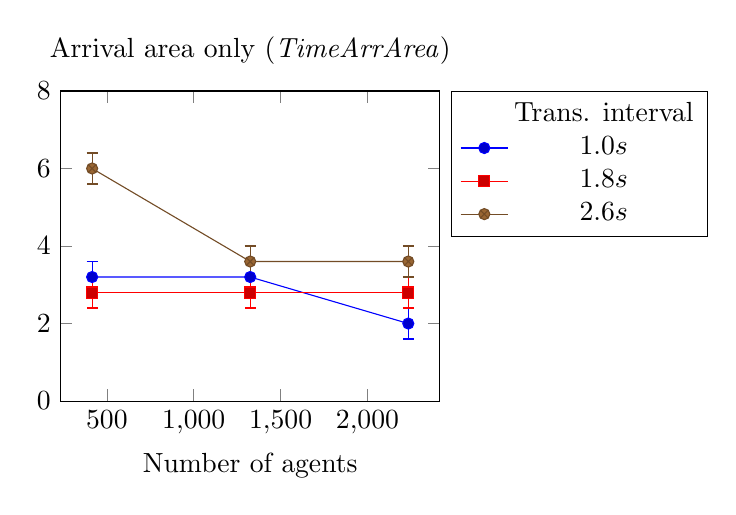
\begin{tikzpicture}
\begin{axis}[xlabel=Number of agents,legend entries={Trans. interval,$1.0s$,$1.8s$,$2.6s$},title=Arrival area only (\textit{TimeArrArea}),ymax=8,ymin=0,width=6.4cm,legend pos=outer north east]
\addlegendimage{empty legend}
\addplot+ [error bars/.cd,y dir=both,y fixed=0.4,
] table [x=Number,y=Area,meta=Time] {
Time Number	All	Area
1.0	415	4.0	3.2
1.0	1325 3.2 3.2
1.0	2235 3.2 2.0
};
\addplot+ [error bars/.cd,y dir=both,y fixed=0.4,
] table [x=Number,y=Area,meta=Time] {
Time Number	All	Area
1.8	415	6.4	2.8
1.8	1325 4.8 2.8
1.8	2235 4.8 2.8
};

\addplot+ [error bars/.cd,y dir=both,y fixed=0.4,
] table [x=Number,y=Area,meta=Time] {
Time Number	All	Area
2.6	415	6.0	6.0
2.6	1325 6.4 3.6
2.6	2235 6.4 3.6
};
\end{axis}
\end{tikzpicture}
\caption[Dissemination time over number of agents]{\textit{Dissemination time} over number of agents. Due to the time step size, the dissemination time has an accuracy of 0.4\,s indicated by the error bars. The data points correspond to the sample points used to construct the polynomial chaos expansions. The dissemination times hardly change over the \textit{number of agents}. The parameter \textit{transmission interval} has indeed an effect (left). }
\label{fig:infodissplotdep}
\end{figure}



The parameter \textit{transmission interval} has a great influence on all quantities of interest. The index is between 0.636 and 0.999 except for the control, see the column `Transmission interval' in Tab~\ref{tab:indicessensit}. An explanation is that the smaller the \textit{transmission interval}, the more often information is provided and the faster the crowd is informed. 
The influence of the \textit{transmission interval} can be also observed in Fig.~\ref{fig:infodissplotdep}. The larger the \textit{transmission interval}, the larger the \textit{information dissemination}. The  parameter influence is more dominant for the entire population than for pedestrians within the arrival area: The corresponding indices are 0.9 (\textit{TimeAll}) and 0.7 (\textit{TimeArrArea}), see again Tab.~\ref{tab:indicessensit}.


To quantify the uncertainty of the \textit{dissemination times}, I look at their statistical moments, see again Tab.~\ref{tab:qoimoments}. One can expect that the total crowd is informed within  5.0\,s ... 5.4\,s, while the population in the arrival area is informed in 3.2\,s ... 3.6\,s. The standard deviations are 1.2\,s and 0.8\,s respectively. Most importantly, none of the \textit{dissemination times} is larger than 7\,s even if the \textit{number of agents} exceeds 2000, see again Fig~\ref{fig:infodissplotdep}.

\subsubsection{Need of repetitive information provision}

With an increasing number of pedestrians, the probabilities of interference and packet loss increase, see Fig.~\ref{fig:interferencepacketloss}. However, interference seems to affect the information dissemination process only locally.  Fig.~\ref{fig:snapshots} shows one sample where some agents have not been informed after 3.6\,s. These agents are all located on the left-hand side near a dense crowd where the risk of interference is high. 
Despite inferences, agents are still informed within 6.4\,s, see Fig.~\ref{fig:snapshots}. I attribute this to the fact that information is provided repeatedly. If the information dissemination fails locally, the information is received in the next broadcast round. Since agents informed in the first round do not forward information, the risk of interference is reduced for the next rounds. This also explains the high influence of the parameter \textit{transmission interval}.




\begin{figure}[hbt!]
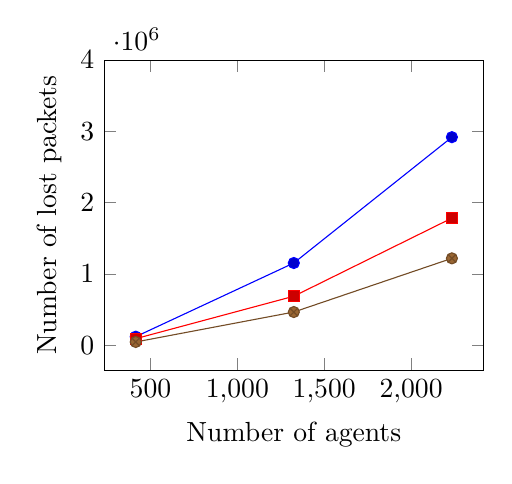
\begin{tikzpicture}
\begin{axis}[xlabel=Number of agents,ylabel=Number of lost packets,width=6.4cm,ymax=4000000]
\addplot+ [] table [x=Agents,y=IncorrectlyReceived] {
id Agents IncorrectlyReceived power
1 415 120407 11
10 1325 1153711 11
19 2235 2918619 11
};
\addplot+ [] table [x=Agents,y=IncorrectlyReceived] {
id Agents IncorrectlyReceived
4 415 92541
13 1325 687913
22 2235 1783373
};
\addplot+ [] table [x=Agents,y=IncorrectlyReceived] {
id Agents IncorrectlyReceived
7 415 46342
16 1325 466153
25 2235 1219119
};
\end{axis}
\end{tikzpicture}
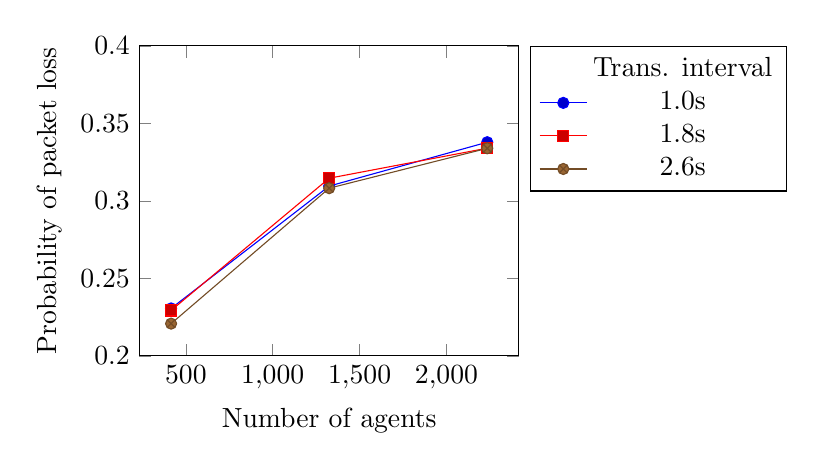
\begin{tikzpicture}
\begin{axis}[xlabel=Number of agents,ylabel=Probability of packet loss,legend entries={Trans. interval,1.0s,1.8s,2.6s},legend pos=outer north east, ymin=0.2, ymax=0.4,width=6.4cm]
\addlegendimage{empty legend}
\addplot+ [] table [x=Agents,y expr=\thisrow{IncorrectlyReceived}/(\thisrow{IncorrectlyReceived}+\thisrow{Passed})] {
id Agents IncorrectlyReceived Passed power
1 415 120407 401675 11 
10 1325 1153711 2573554 11
19 2235 2918619 5720886 11
};
\addplot+ [] table [x=Agents,y expr=\thisrow{IncorrectlyReceived}/(\thisrow{IncorrectlyReceived}+\thisrow{Passed})] {
id Agents IncorrectlyReceived Passed power 
4 415 92541 310980 11 
13 1325 687913 1498629 11
22 2235 1783373 3556361 11
};
\addplot+ [] table [x=Agents,y expr=\thisrow{IncorrectlyReceived}/(\thisrow{IncorrectlyReceived}+\thisrow{Passed})] {
id Agents IncorrectlyReceived Passed power
7 415 46342 163505 11
16 1325 466153 1046453 11
25 2235 1219119 2431961 11
};
\end{axis}
\end{tikzpicture}

\caption[Packet loss caused by interference]{ Packet loss caused by interference. The number of lost packets increases over the \textit{number of agents} (left). The lower the transmission interval, the more often the dissemination process is re-started and the higher the loss is. The probability for interference, estimated by the the number of lost packets divided by the number of total packets, also increases over the \textit{number of agents} (right). The transmission interval has no effect on the probability.  }
\label{fig:interferencepacketloss}
\end{figure}





\begin{figure}[hbt!]
\begin{tikzpicture}
\node[inner sep=0pt] at (0,0){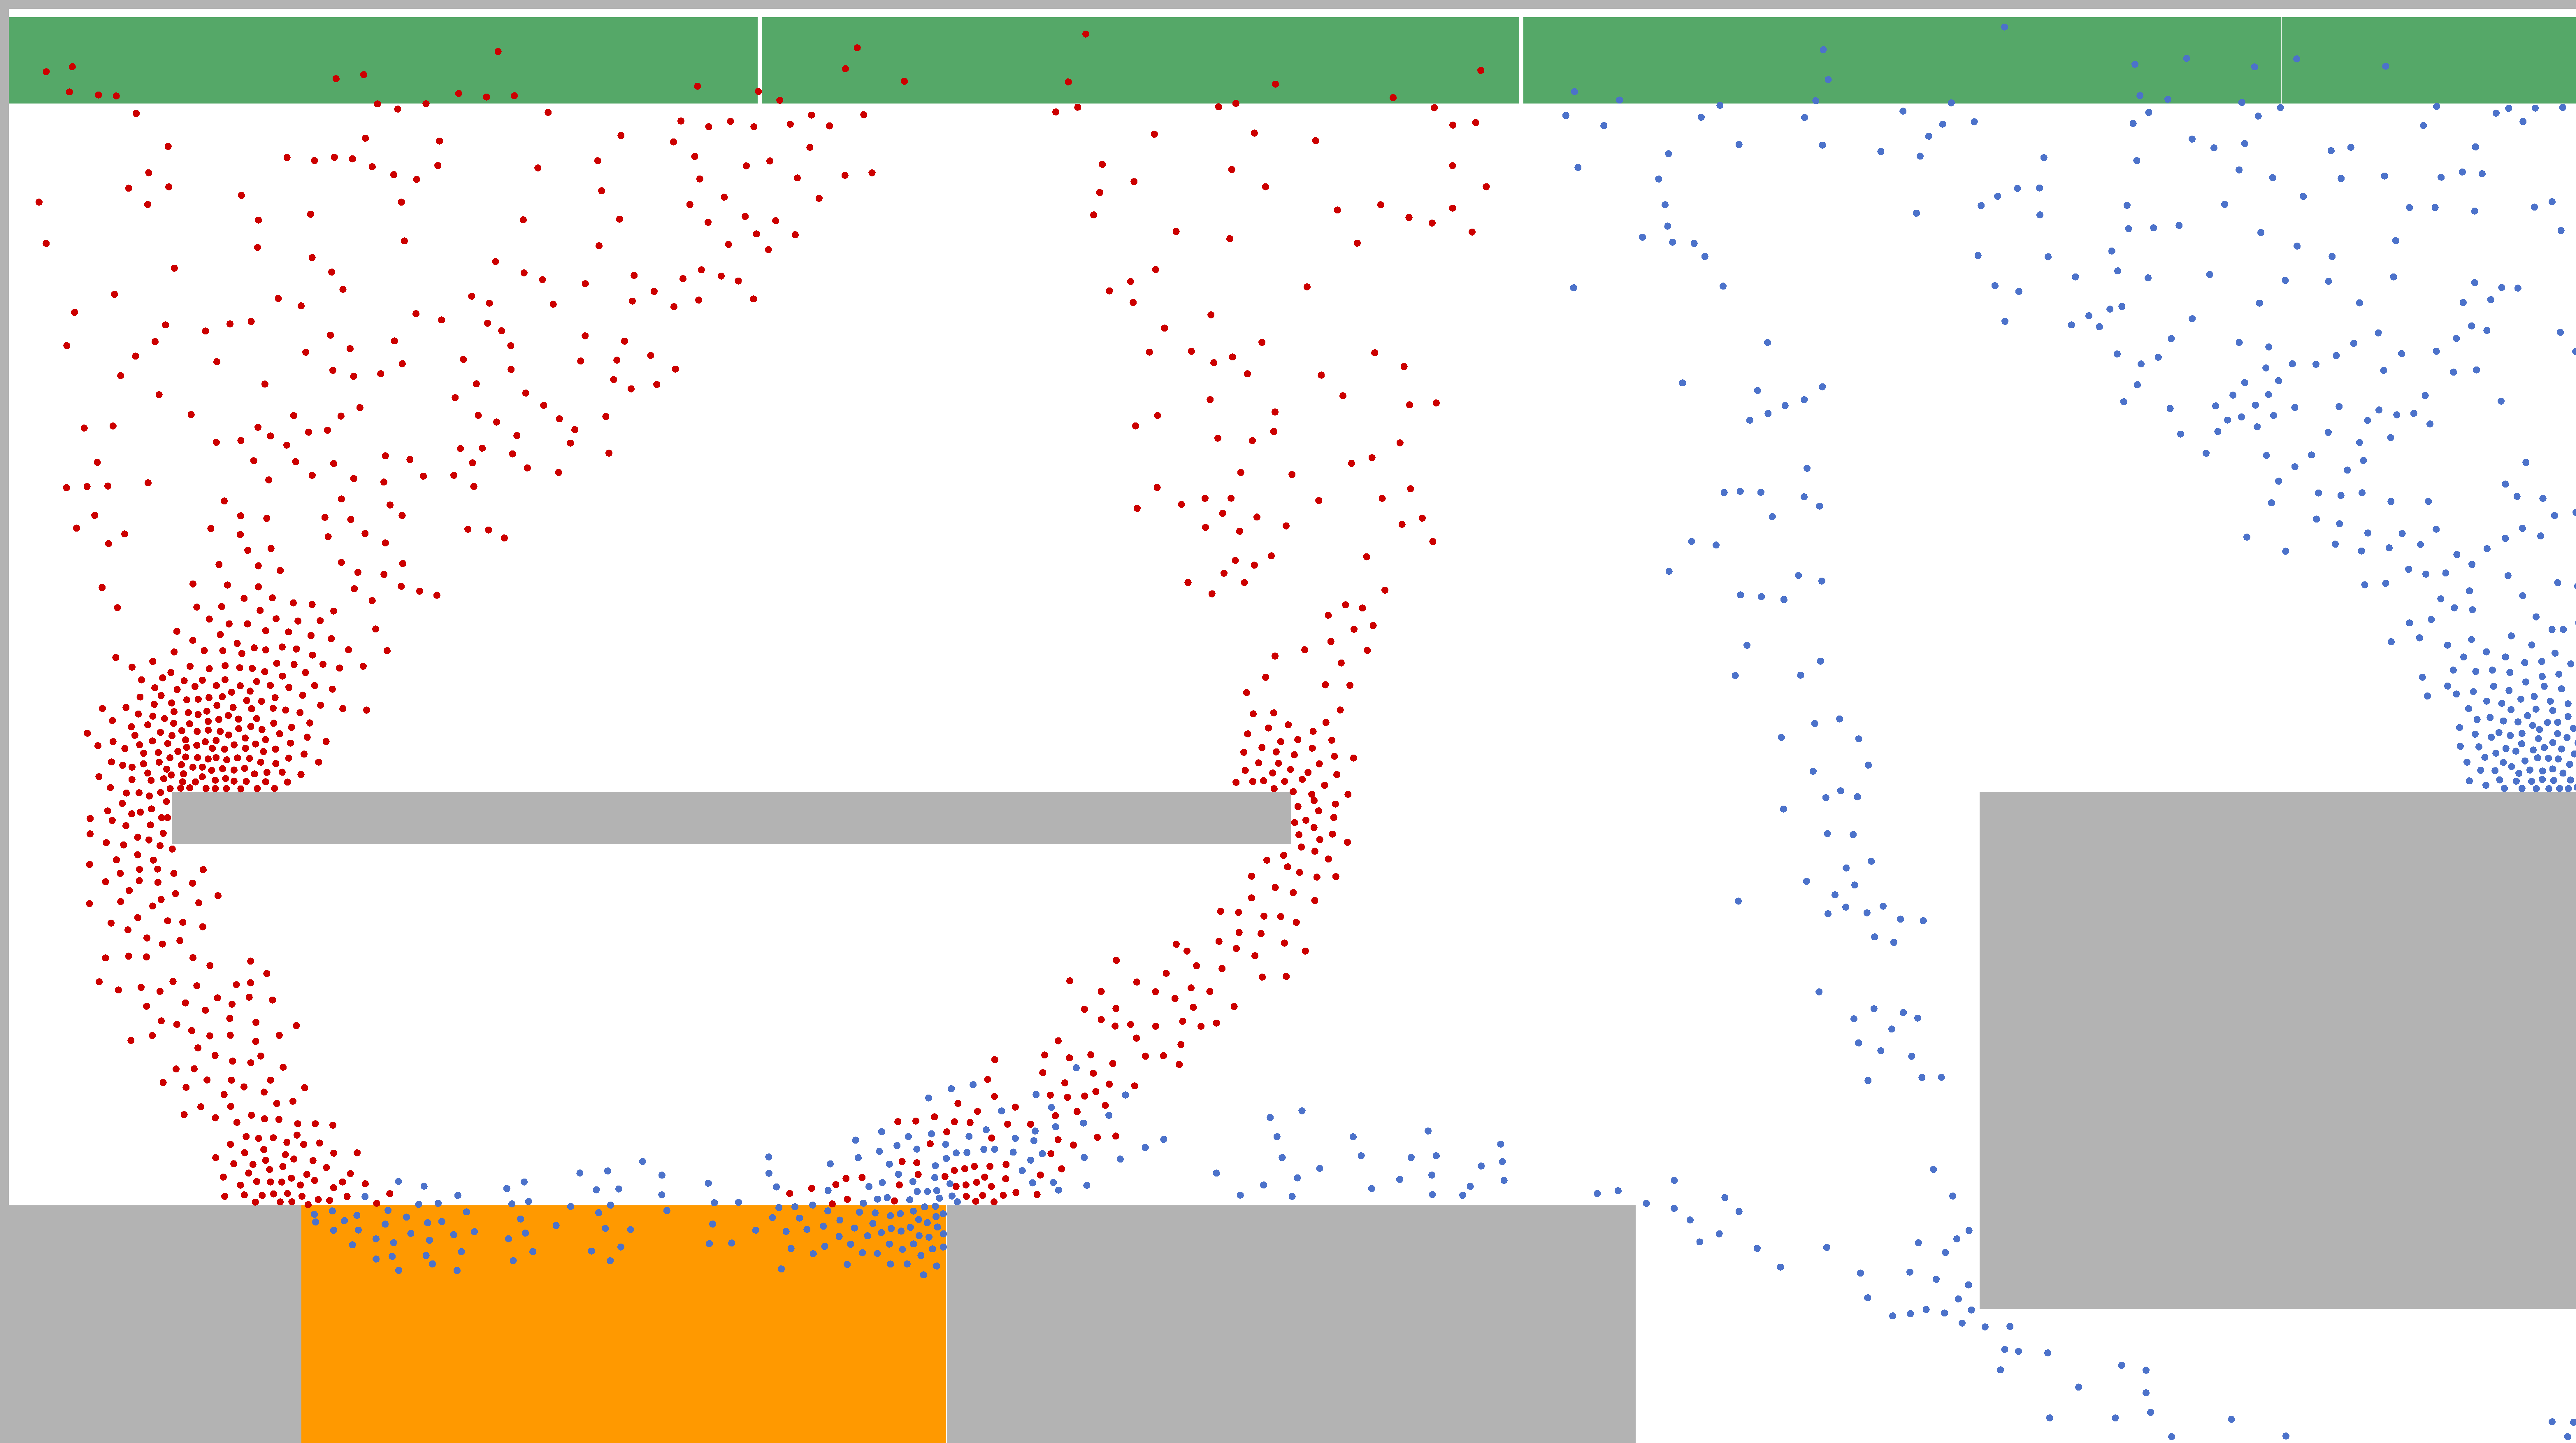
\includegraphics[width=9cm]{./investigation/Informationsverbreitung/Sample_26/info_diss_sample_26_100s_state_part.pdf} };
\node[inner sep=0pt] at (0,-5.5){\includegraphics[width=9cm, trim=0cm 35cm 30.0cm 0cm, clip]{./investigation/Informationsverbreitung/Sample_26/info_diss_sample_26_103_6s_area_informed_part.pdf}};
\node[inner sep=0pt] at (0,-11){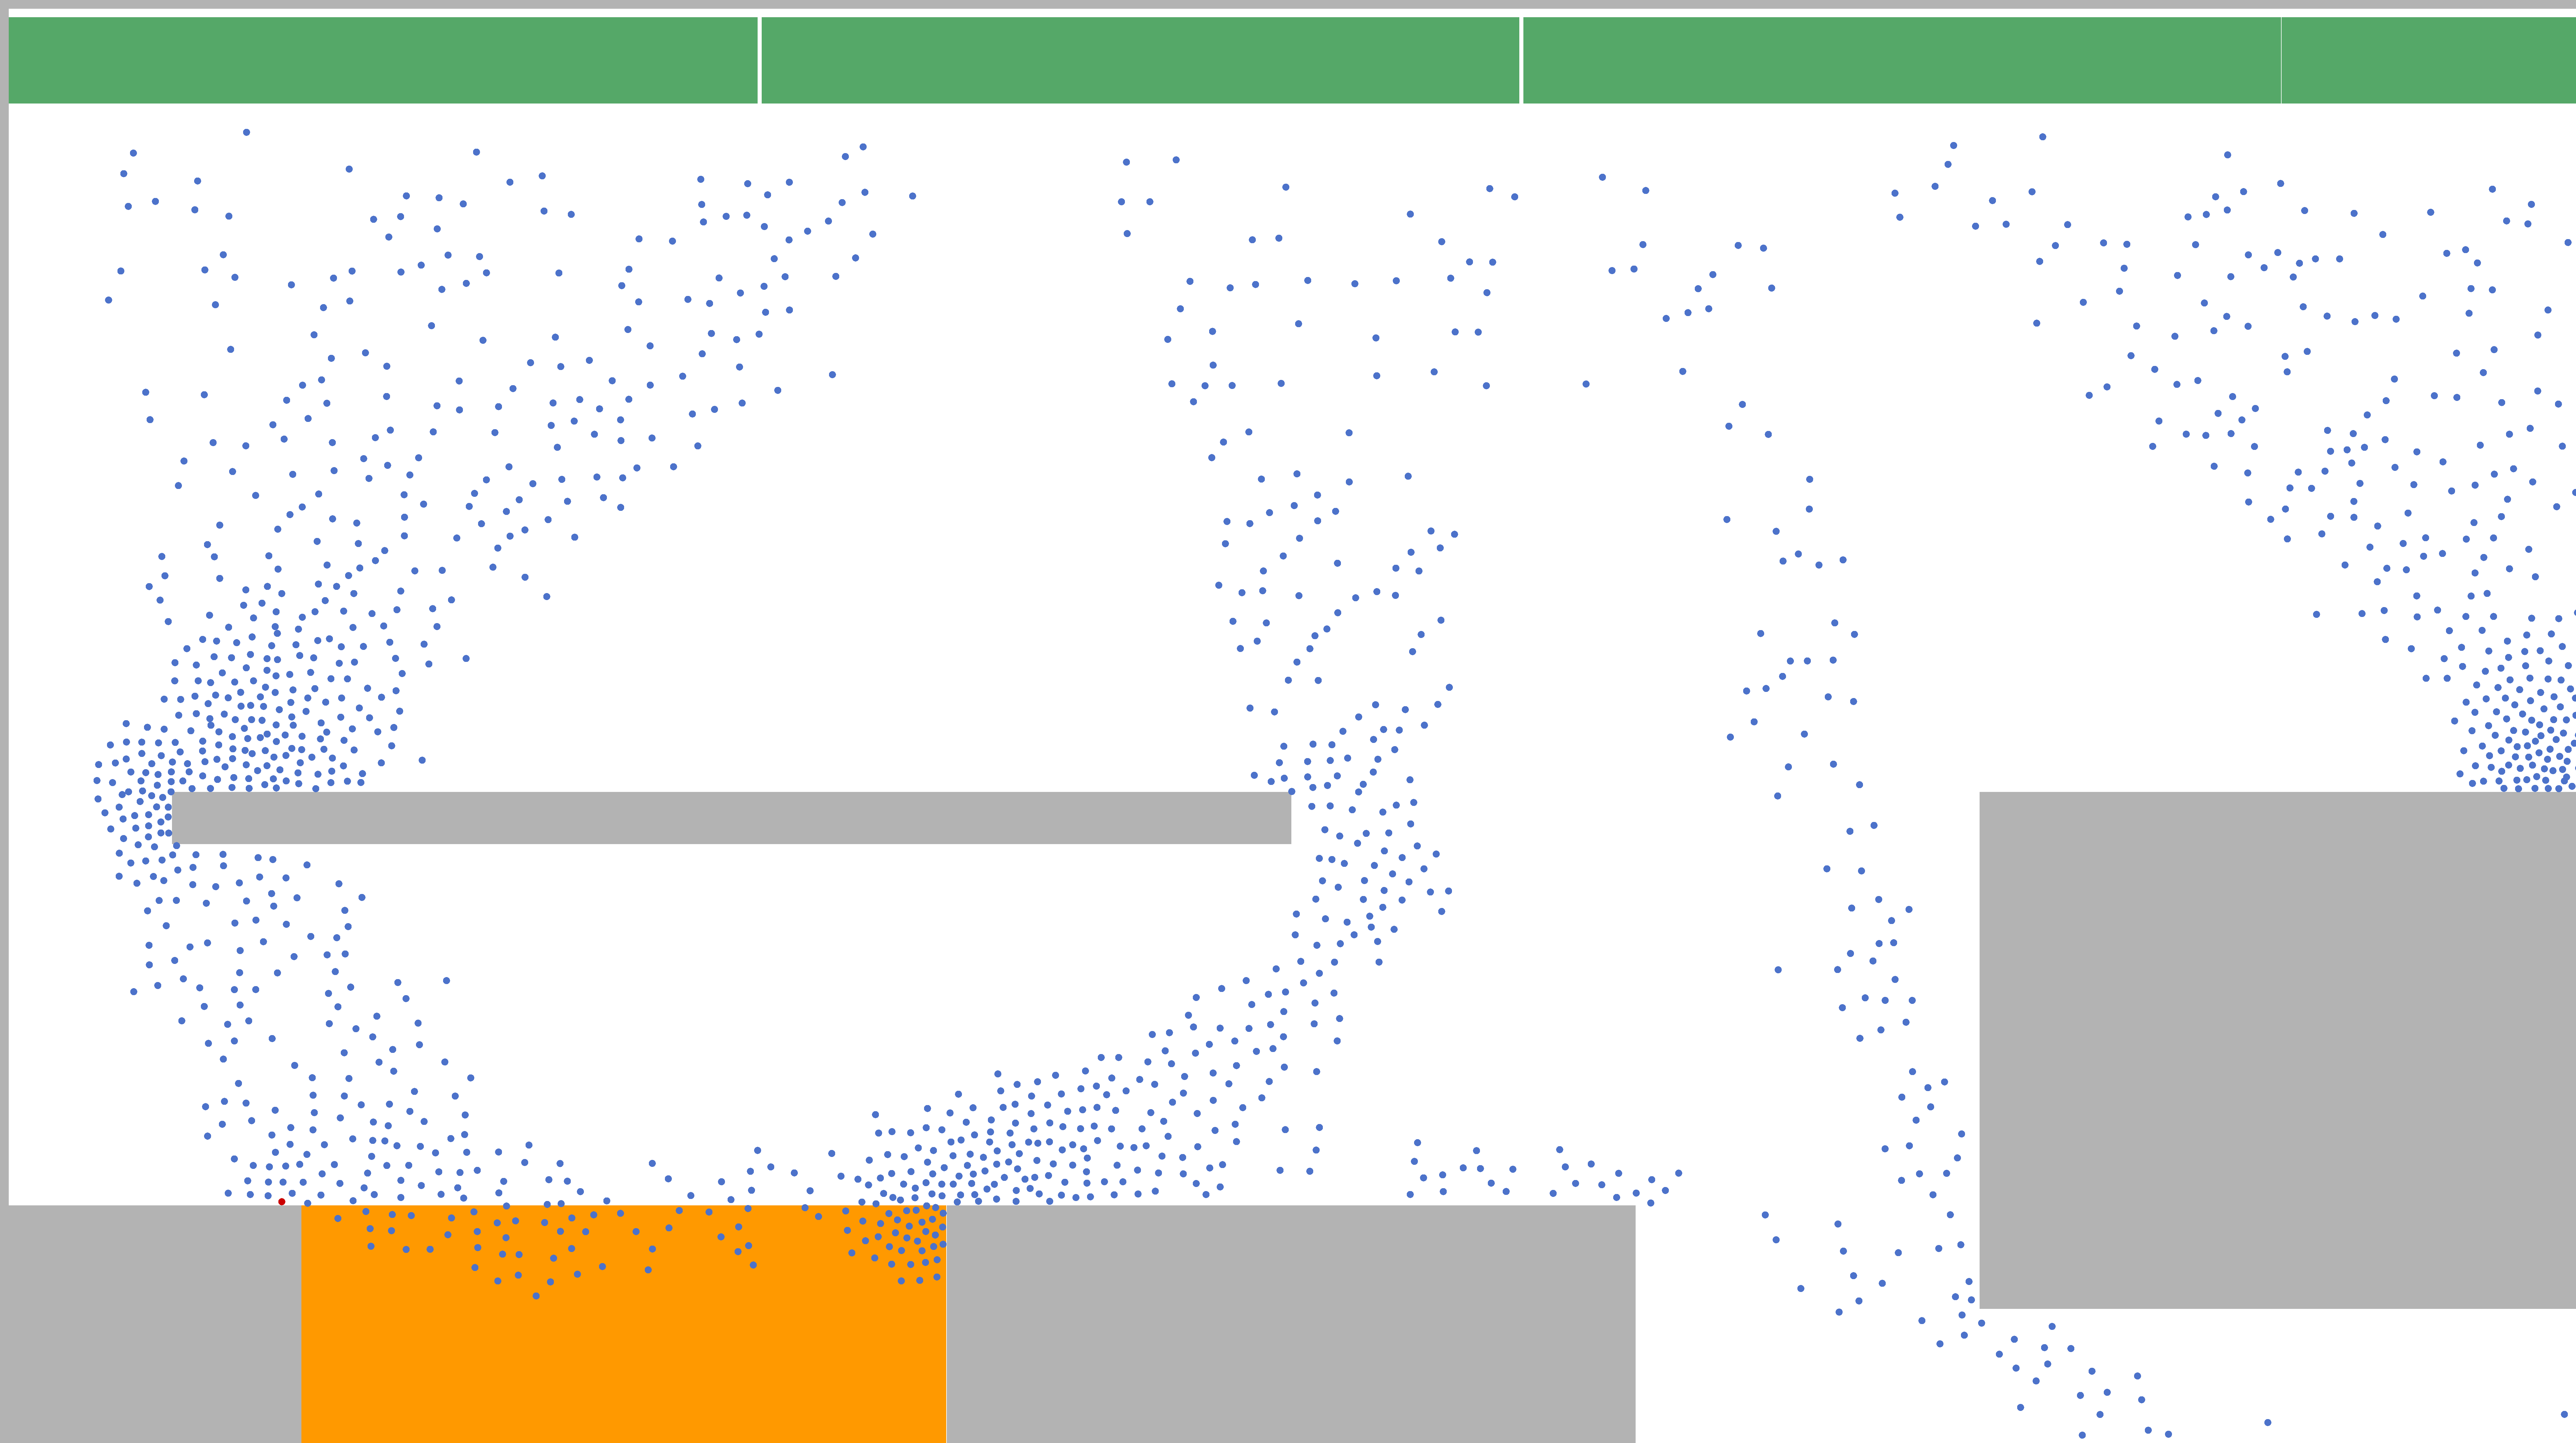
\includegraphics[width=9cm]{./investigation/Informationsverbreitung/Sample_26/info_diss_106_4_all_informed_part.pdf}};
\node[text width =7cm] at (8.5,0) {Simulation time: 100.0\,s \\ (Start to disseminate information)};
\node[text width =7cm] at (8.5,-5.5) {Simulation time: 103.6s \\ (95\,\% of agents informed \\ in arrival area)  };
\node[text width =7cm] at (8.5,-11) {Simulation time: 106.4s \\ (95\,\% of agents informed) };

\draw (-3.8,-6.7) circle (0.7);
\node[text width=3.4cm] at (-1.1,-6.5) {Agents not \\ informed yet (red)};

\draw[draw=black, dashed] (-4.5,-5.3) rectangle ++(9,2.0);
\node[text width=8cm] at (0,-3.8) {Arrival area: $>$ 95\,\% of agents informed };


\end{tikzpicture}
\caption[Uncertainty quantification study: Simulation snapshots ]{ Uncertainty quantification study: Simulation snapshots for the design with 2235 agents, a transmitter power of 19.97\,mW and a transmission interval of 2.6\,s. The information dissemination starts at 100\,s. Red agents are unaware about the closure of the gate. After 3.6\,s, the agents in the upper part have been informed. After 106.4\,s 95\,\% of the total population has been informed. }
\label{fig:snapshots}
\end{figure}


\subsubsection{Delays in the information dissemination process}
As expected, the sub-population of agents in the arrival area is informed faster than the total population. Fig.~\ref{fig:infodegree} depicts the information degree for both populations. One can observe that the orange lines (sub-population) cross the 95\,\% threshold earlier than the blue lines (total population). This is plausible, since less agents need to be informed. Interestingly, the information dissemination process shows some delays, see the  plateaus of the graphs in Fig.~\ref{fig:infodegree}. These delays occur because the information is passed via a chain of agents around obstacles. If the communication chain breaks, the transmission is delayed for at least one \textit{transmission interval}. Note that, for the arrival area, the decrease of the information degree in Fig.~\ref{fig:infodegree} (top left) is caused by informed agents leaving the arrival area. 



\begin{sidewaysfigure}
%\thisfloatpagestyle{empty}
\begin{tikzpicture}
\node[inner sep=0pt] at (0,0){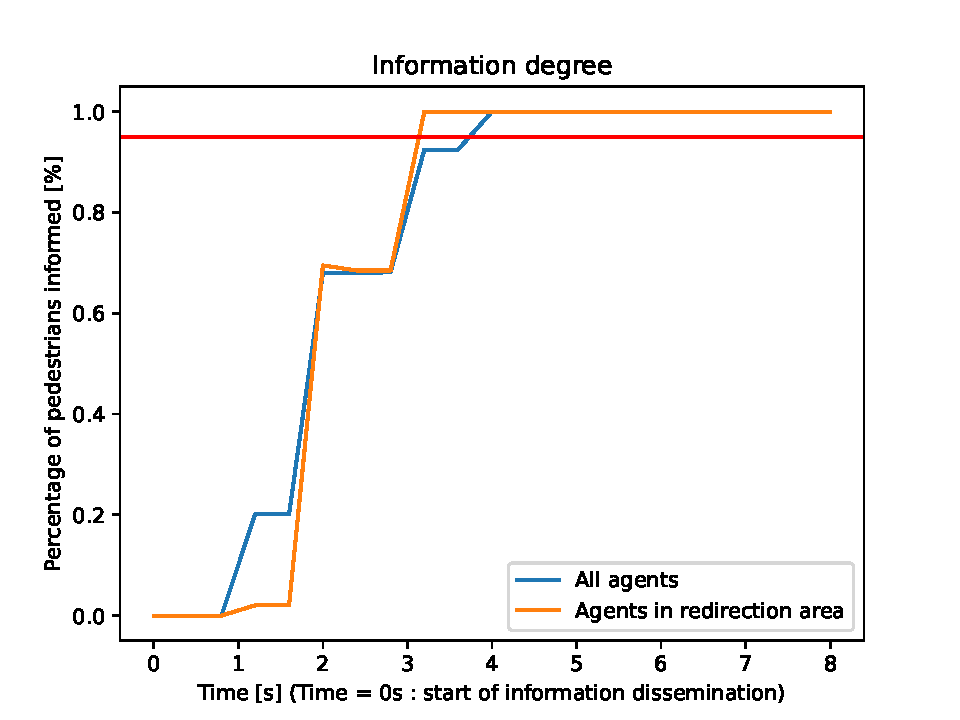
\includegraphics[width=7.5cm]{./investigation/crownetOutput/information_diss_time/InformationDegree_Sample_1_0.pdf}};
\node[inner sep=0pt] at (7,0){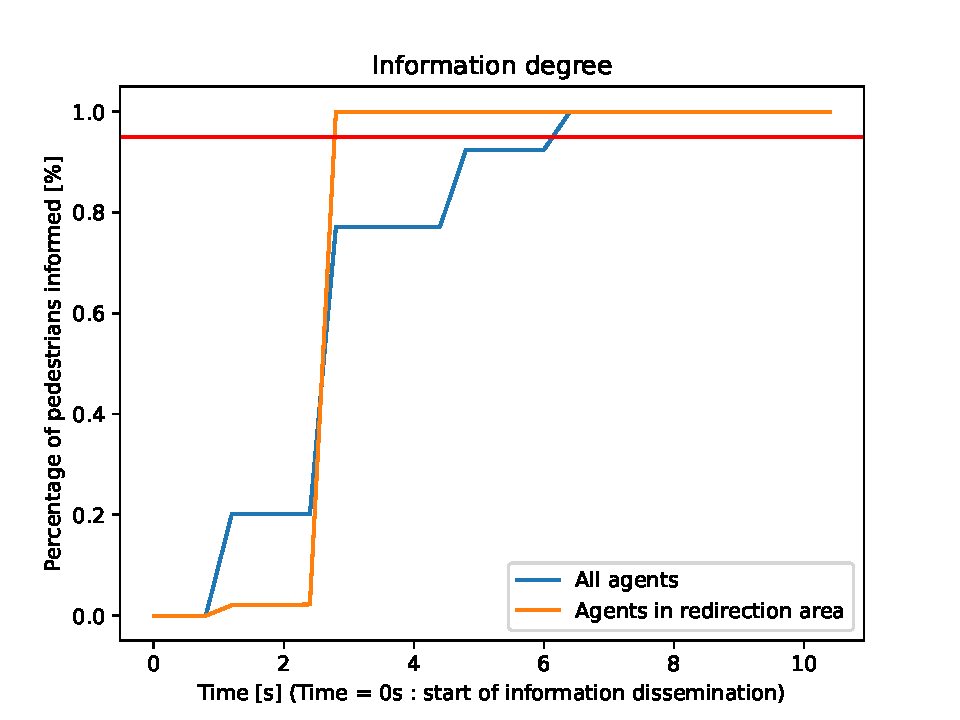
\includegraphics[width=7.5cm]{./investigation/crownetOutput/information_diss_time/InformationDegree_Sample_4_0.pdf}};
\node[inner sep=0pt] at (14,0){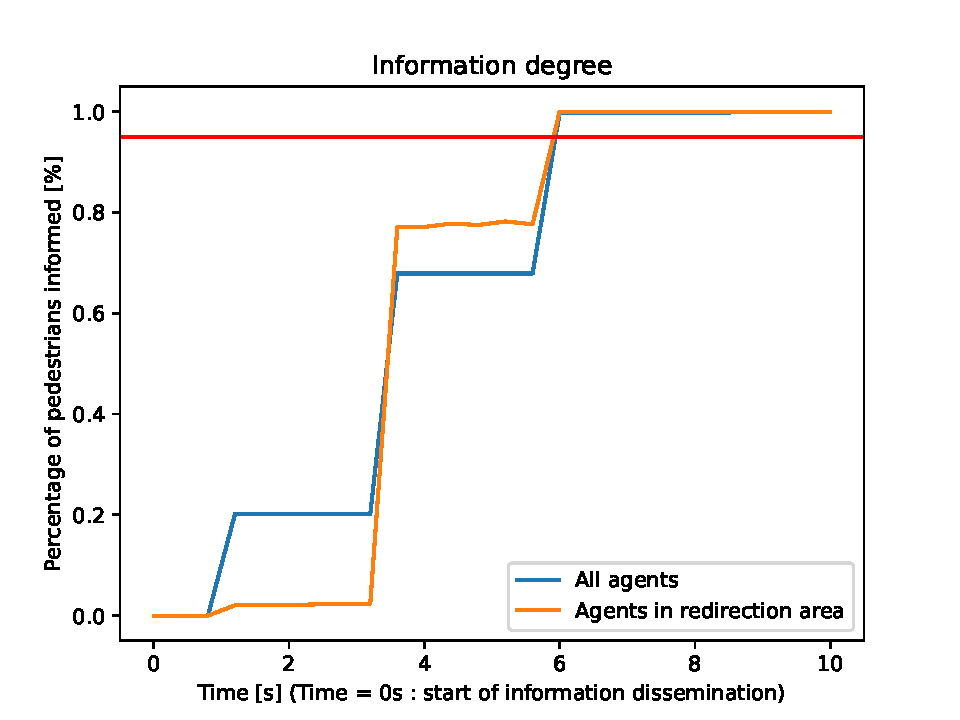
\includegraphics[width=7.5cm]{./investigation/crownetOutput/information_diss_time/InformationDegree_Sample_7_0.pdf}};
\node[inner sep=0pt] at (0,-5.1){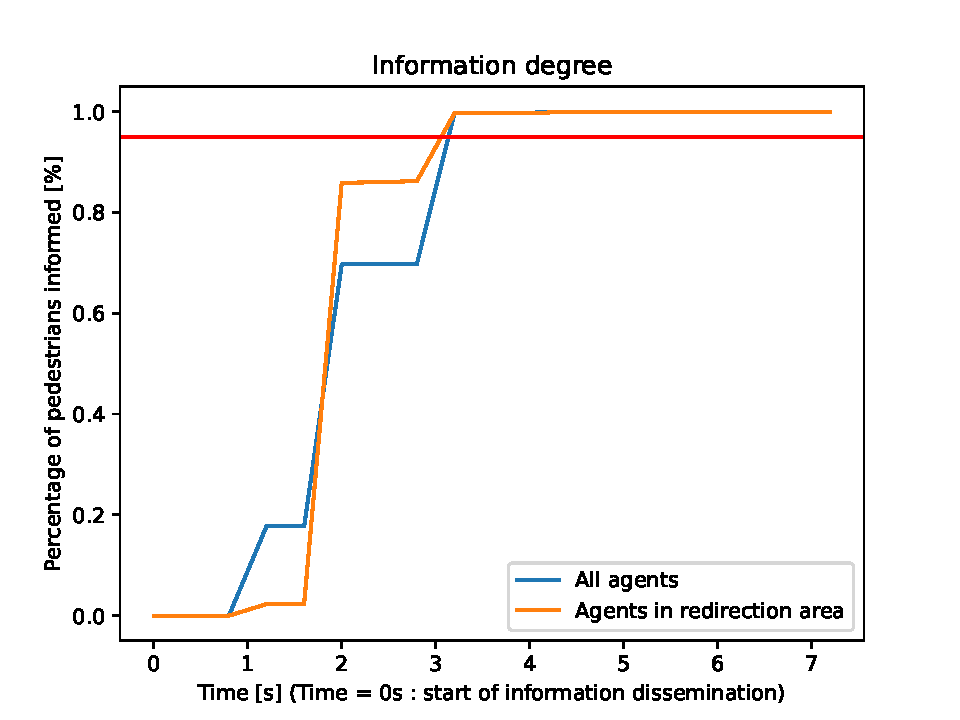
\includegraphics[width=7.5cm]{./investigation/crownetOutput/information_diss_time/InformationDegree_Sample_10_0.pdf}};
\node[inner sep=0pt] at (7,-5.1){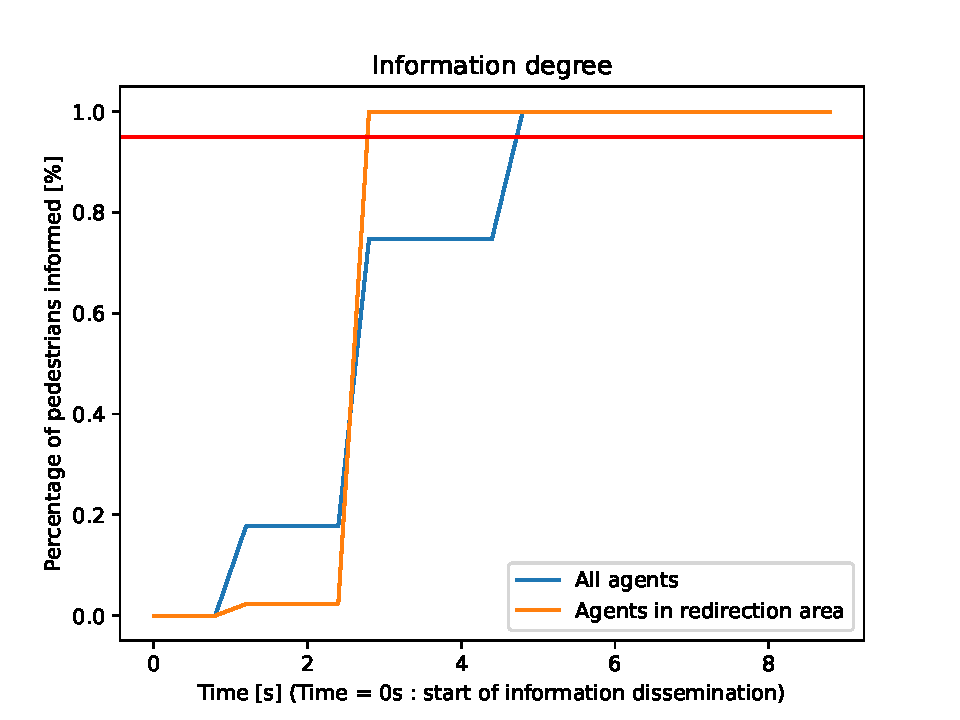
\includegraphics[width=7.5cm]{./investigation/crownetOutput/information_diss_time/InformationDegree_Sample_13_0.pdf}};
\node[inner sep=0pt] at (14,-5.1){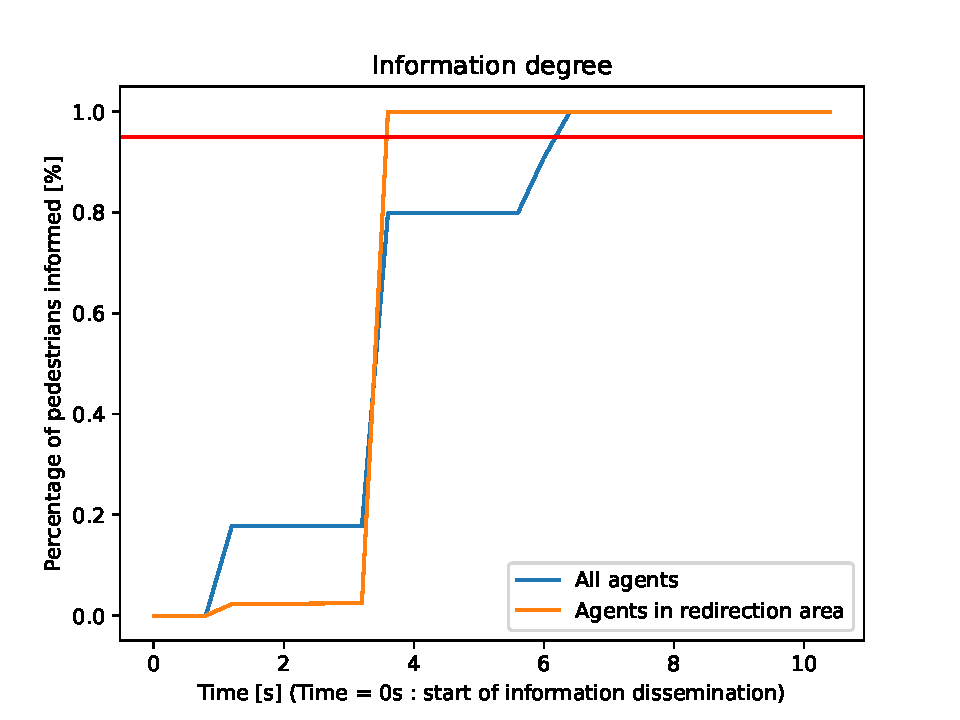
\includegraphics[width=7.5cm]{./investigation/crownetOutput/information_diss_time/InformationDegree_Sample_16_0.pdf}};
\node[inner sep=0pt] at (0,-10.2){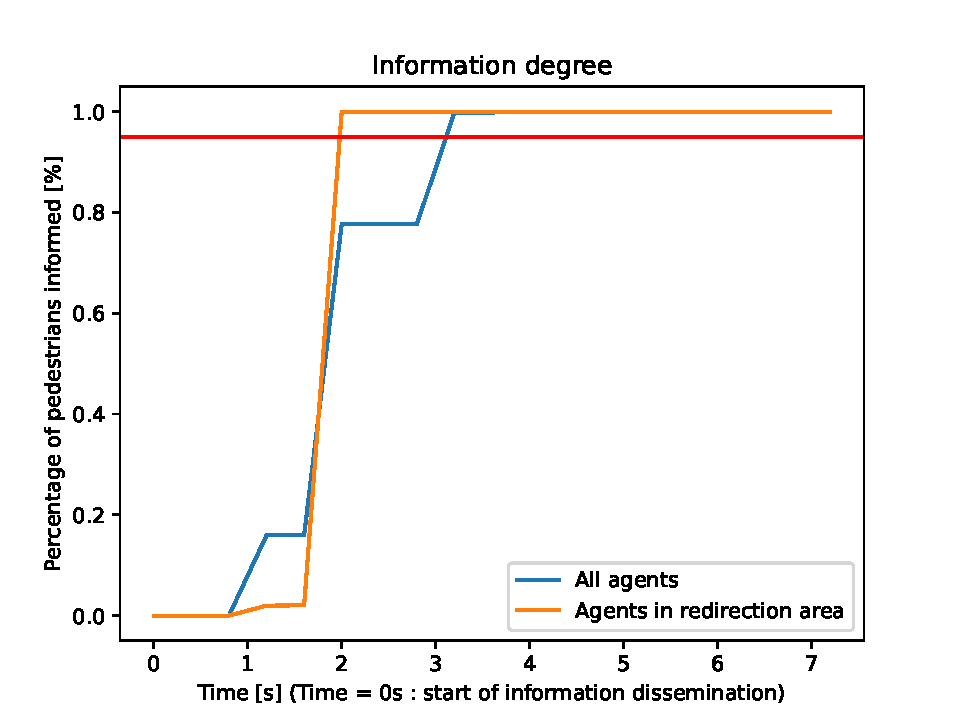
\includegraphics[width=7.5cm]{./investigation/crownetOutput/information_diss_time/InformationDegree_Sample_19_0.pdf}};
\node[inner sep=0pt] at (7,-10.2){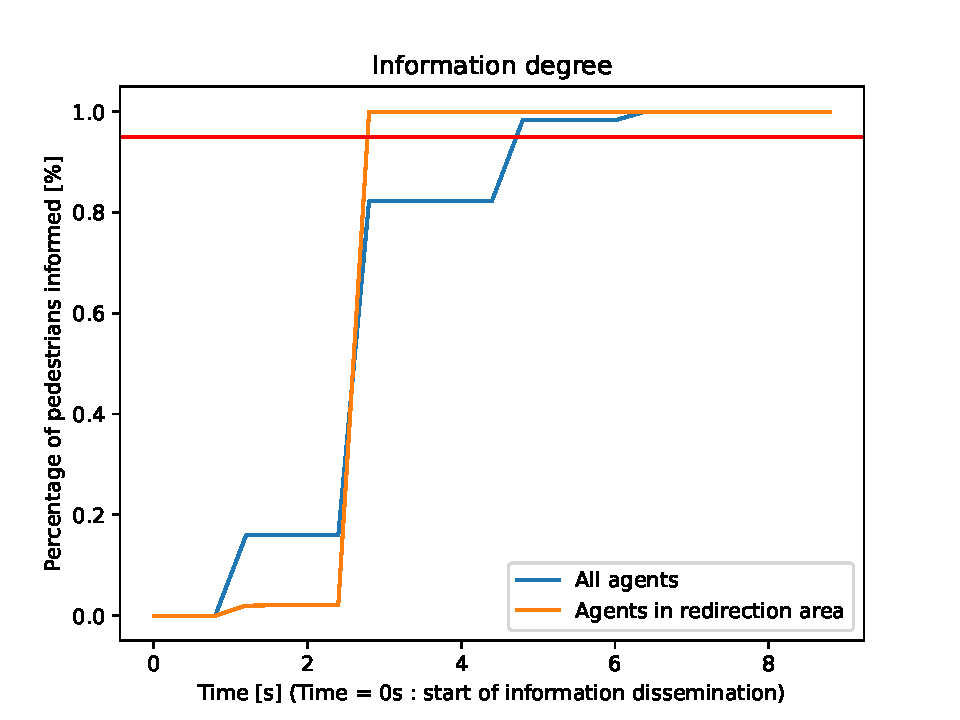
\includegraphics[width=7.5cm]{./investigation/crownetOutput/information_diss_time/InformationDegree_Sample_22_0.pdf}};
\node[inner sep=0pt] at (14,-10.2){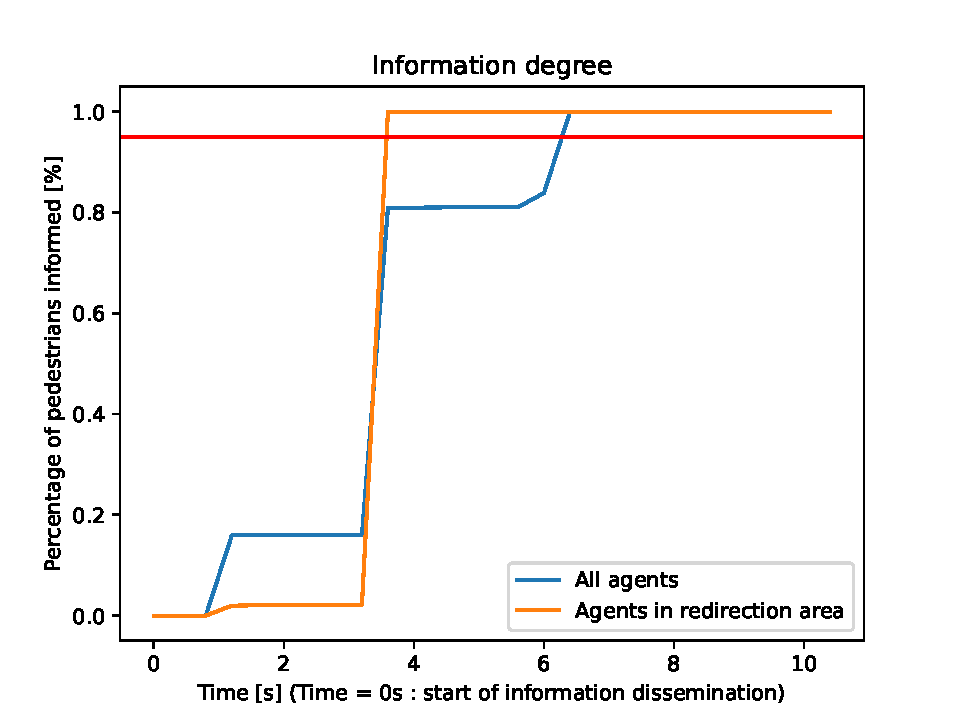
\includegraphics[width=7.5cm]{./investigation/crownetOutput/information_diss_time/InformationDegree_Sample_25_0.pdf}};
\node[text width =7cm] at (11,3.4) {\textbf{Transmission interval}};
\node[text width =7cm] at (3,3) {1.0\,s};
\node[text width =7cm] at (11,3) {1.8\,s};
\node[text width =7cm] at (17,3) {2.6\,s};
\node[text width =7cm] at (-1,0) {415};
\node[text width =7cm] at (-1,-5.1) {1325};
\node[text width =7cm] at (-1,-10.2) {2235};
\node[text width =2cm] at (-4.7,1) {\textbf{Number of agents}};
\end{tikzpicture}
\caption[Information degree over time for a fixed radio transmitter power]{Information degree over time for a fixed radio transmitter power (p\,=\,11\,mW). The information dissemination time is the time that elapses until 95\,\% of the agents are informed in the arrival area (orange curve) or the total area (blue curve). The value p\,=\,95\,\% (red line) ensures that temporal fluctuations, caused by informed agents leaving one of the reference areas, do not have an effect.}
\label{fig:infodegree}
\end{sidewaysfigure} 



\subsubsection{Summary and findings from the uncertainty quantification analysis}
The second sub-study indicates that information can be disseminated in a mobile crowd through direct communication within a few seconds. A global sensitivity analysis showed that the crowd size does not greatly affect the dissemination time, that is, the time it takes to distribute detour information in a crowd. This is fortunate since in a real life application one cannot control the crowd size. The transmission interval, that is the time between two repetitions when detour information is sent, had a big influence on the information dissemination process. The more often information was provided, the faster the entire crowd was informed. 
 
\FloatBarrier

\subsection{Summary, limitations, lessons learned}

\subsubsection{Summary of the two investigations}

In this section I investigated my first research sub-question, that is, how reliably route recommendations are disseminated through direct communication technology in a mobile crowd.
I proposed and applied a two-step procedure to investigate the information dissemination systematically when shadowing is present. First, one examines how shadowing depends on the number of agents in the scenario.  More agents mean a closer distance between nodes in the mobile network. Second, one assesses how quickly information is transmitted when there are sufficiently many crowd members in the system. This procedure allows to separate the effect of shadowing and interference and, thus,  helps to better understand the behavior of the socio-technical system composed of the crowd and the mobile network. To answer my research question, I designed a scenario that reflects worst-case conditions for the direct communication: A person sending the detour information was shadowed by walls and only pedestrians in line-of-sight received detour information through direct communication.
To evaluate the reliability of the information dissemination process, I introduced a criterion that demands that the entire crowd must be informed within a certain time. 
In the first part of the study I varied the number of agents. I found that at least 110 crowd members are necessary to prevent shadowing in the scenario. In the second part, the uncertainty of the information dissemination process was quantified using forward propagation based on polynomial chaos expansions. To quantify the influence of parameters, global sensitivity analysis was applied, again using polynomial chaos expansions. I found that route recommendations were disseminated in a crowd within a few seconds. The number of crowd members had a low effect on the information dissemination when the crowd was dense enough. The transmission interval, that is the time in between two information broadcasts, had a large effect on the information dissemination. The more often information was provided, the faster the entire crowd was informed. In my scenario the fastest information dissemination was achieved with a transmission interval of one second. 


In both studies I assumed that the communication breaks whenever the line-of-sight is broken. In reality, the information provision might be even better thanks to the permeability of materials and to reflections. In short the answer to the first research sub-question is:

\begin{tcolorbox}[title=How reliably are route recommendations disseminated using direct communication in a crowd? (RQ-1)]
Using direct communication technology, route recommendations can be reliably disseminated in a mobile crowd  within a few seconds, provided there are enough crowd members to counteract shadowing.
\end{tcolorbox}



\subsubsection{Limitations}
I would like to point out some limitations of the study, some of them which I will address in my following investigations.


I assumed that all pedestrian immediately and always follow the route recommendation. In reality, pedestrians might not be aware of the mobile message or for some reason my not follow instructions. Therefore, I will assess the effect of compliance in Section~\ref{sec:umleitalgorithmen}.

The topography of the scenario was sufficiently small. Therefore, pedestrian were always in communication range. If the topography was larger, information dissemination may fail.

In the study, interference caused local packet loss which did not affect the overall information dissemination process. However, if the crowd size was denser, information dissemination might fail. 

In the study I tested direct communication based on the WLAN 802.11p standard. I did not look at more advanced technologies, such as 802.11bd communication or cellular sidelink communication, because I wanted to assess the worst case. For example, I expect that the risk of interference is smaller for the sidelink communication in the controlled mode. Therefore, I am optimistic that other technologies are also suitable: I will test LTE sidelink communication in Section~\ref{sec:realistiscscenario}.

I excluded additional network traffic to keep the numbers of factors low in the study. As a previous study shows, network load has indeed an effect on the information dissemination, see Appendix~\ref{sec:effectofnetworktraffic}. I argue that a network load through direct communication is unlikely to occur in real life applications because people use mobile applications that request individual data. There is no need to share data between devices. Hence people use conventional cellular communication. Due to other frequency bands, the direct communication would not be affected.

I only analyzed the effect of three uncertain parameters that I identified as main model parameters. There is always the possibility that I may have overlooked an important uncertain parameter. 



\subsubsection{Lessons learned for my further investigations}



The study showed that the crowd size slightly affects the information dissemination given that the crowd is dense enough and well-distributed. Route recommendation algorithms are in particular interest for dense crowds. From this, I~conclude that such an algorithm does not need to take the crowd size into account.

In the study, the transmission interval was varied. Although it had an effect on the information dissemination, the crowd was always informed within a few seconds. I~conclude that an interval on a second scale is sufficient when information needs to be provided repeatedly due to an information loss.

In the study, the information dissemination took longer than the size of one transmission interval. Therefore, a route recommendation algorithm that generates recommendations dynamically must not change the information content during this period of time. Otherwise, contradictory information could be disseminated. I conclude that it is essential to check whether this functional requirement is fulfilled. I will present a procedure for this in Section~\ref{sec:realistiscscenario}.









\section{Selection of a route recommendation algorithm}

\label{sec:umleitalgorithmen}

In this section I investigate my second research sub-question: Which algorithms are suitable for generating route recommendations for crowds, given not all people follow instructions?
In the state of the art, I  discussed why former algorithms were tested under unrealistic conditions: It was assumed that crowds behave like fluids. However, recommending a route is not the same as opening a valve to regulate fluid flows. People may or may not follow instructions that are suggested to them by signs, loudspeakers, mobile applications or staff. This is true even if they perceive and understand the suggestions. For this reason, it is necessary to consider the influence of compliance when investigating route recommendation algorithms. In view of the models’ and, indeed, the true systems’ many uncertainties, I argue that simple algorithms have a better chance to be implemented in a real setup than more intricate algorithms. I also expect algorithms to be more robust if they do not depend on precise measurements to achieve target values in some control loop. This is why I propose and test three heuristic algorithms for unknown compliance rates. The study presented in this section builds on my publication~\textit{Guiding crowds when facing limited compliance: Simulating strategies}~\cite{mayr-2022-cdyn}
in which I examined two out of three route recommendation algorithms from this study. The careful reader will therefore find textual overlaps, as the studies have a similar structure. Since this study extends the findings from my previous study, it is also of interest for readers who are already familiar with the publication.



\subsection{Research scenario}

I propose a scenario inspired by a real-life use case at the metro station Münchner Freiheit in Munich, Germany. For the purpose of this study, it is sufficient to know that there are three routes of different lengths at Münchner Freiheit station to get from the bus or tram to the trains. The short route is usually more occupied than the two alternatives. This leads to congestion especially before football matches when fans change trains. The station site extends over two floors, which are connected through escalators, a ramp and stairs. 
%Due to that, there are heterogeneous traffic conditions along the three different routes. 
To understand the effect of compliance and the difference between algorithms, effects caused by local topographical features such as  twists and turns, stairs or surface conditions, are excluded. Such local effects would introduce additional factors, which might prevent me from clearly assigning an effect to a factor. I, therefore, use an abstracted model of the topography.

The topography is depicted in Fig.~\ref{fig:designumleitalg}. The outer dimensions of the area are 150\,m $\times$ 25\,m. The corridor widths and the ratio of the route lengths are similar to the real use case. The corridor width is w = 2.5\,m for all corridors. Every two seconds, eight agents are spawned in the source on the left. The agents try to reach the (orange) targets placed at the ends of each corridor on the right. Without guidance, all agents take the shortest route, that is, the corridor on top. Such a behavior can be observed for football fans in the real world scenario. Congestion occurs along and in front of the short route. 

To relieve the congestion, a crowd guidance system is implemented. The system provides route recommendation for agents within the information area. Agents follow a route recommendation with a probability $c$, that is, the compliance rate.


\begin{figure}[hbt!]
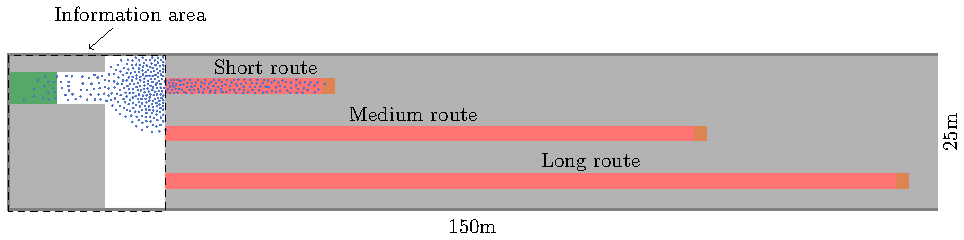
\includegraphics[width=\textwidth]{figures/investigation/VergleichUmleitalgorithmen/Scenario.pdf} 
%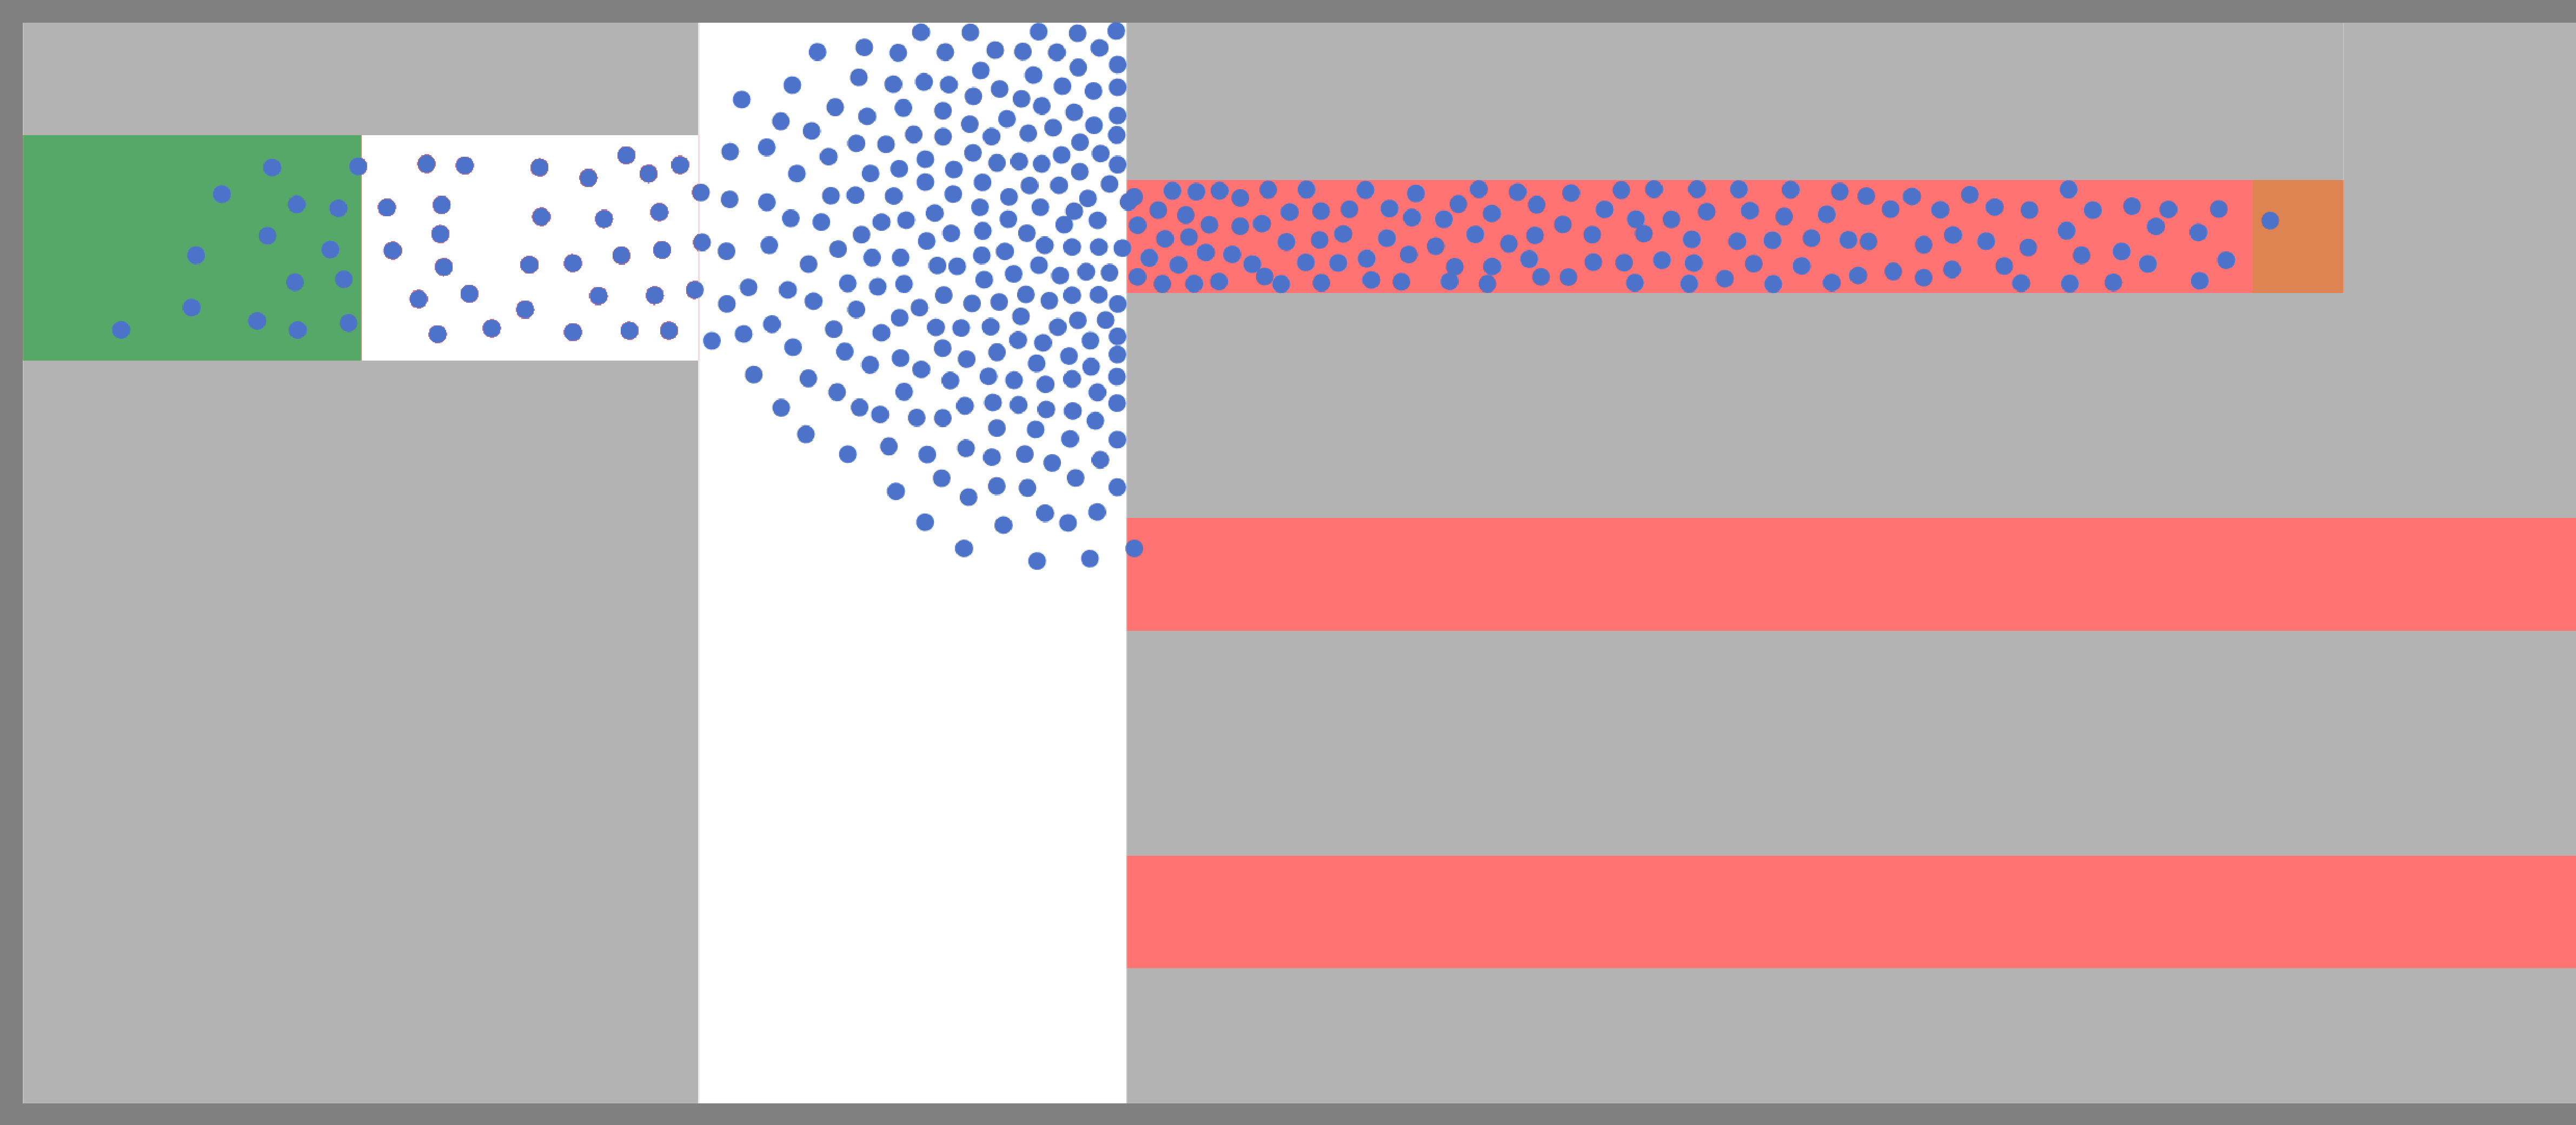
\includegraphics[width=\textwidth]{figures/investigation/VergleichUmleitalgorithmen/StausituationOhneUmleitung.pdf}
\caption[Simplified topography]{Simplified topography. Agents are spawned in the source on the left (green) and walk to the targets (orange) on the right end of each corridor. Without guidance, all agents take the short route which causes congestion along and in front of the short route. In the setting with guidance, agents receive a route recommendation in the information area.  Only a proportion of the crowd follows the route recommendation.}
\label{fig:designumleitalg} 
\end{figure}




\subsection{Setup of the simulation model and implementation}


The simulation model of the crowd guidance system is composed of several component models, see Tab.~\ref{fig:composedmodelrq-2}. The validated Optimal Steps Model is used to model the locomotion behavior of the crowd. For the route recommendation algorithm and the route choice behavior, I propose novel models that are presented in the following. 


\begin{table}[hbt!]
\begin{footnotesize}
\begin{tabular}{p{2cm}p{4cm}p{7cm}}
\hline
Model & Sub-model & Model (simulator) \\ \hline
Crowd  & Locomotion model & Optimal Steps Model (Vadere) \\
& Perception model &  SimplePerceptionModel (Vadere) \\
& Cognition model & ProbabilisticCognitionModel (Vadere) \\
Controller &
Time stepping alg. & FixedTimeStepper  (flowcontrol) \\
&  Route recommendation alg. & AlternateTargetAlgorithm  (flowcontrol) \\
&& \textbf{OR} \\
 && MinimalDensityAlgorithm    (flowcontrol) \\
 && \textbf{OR} \\
 &&  AvoidCongestionAlgorithm (flowcontrol) \\
Network & None & Assumption: information arrives immediately   \\ \hline
\end{tabular} 
\end{footnotesize}
\caption[Composed model for investigating guiding strategies]{Composed model for investigating guiding strategies. }
\label{fig:composedmodelrq-2}
\end{table}

\subsubsection{Route recommendation algorithms}
The route recommendation algorithm dynamically generates route recommendation at a certain time interval. Agents perceive these route recommendations only within the information area that is composed of the green area
of the source and the white area between the source and corridors, see Fig.~\ref{fig:designumleitalg}. 

I choose a time interval of $\Delta t=$2\,s. The smaller the time interval, the more the algorithm is able to react to changes in the dynamics. In an ideal world, where agents would react immediately and reliably, one would expect a smaller $\Delta t$ to improve the distribution of agents. However, through the delay caused by the provision of information and the fact, that it might be confusing for pedestrians when the information content changes rapidly, I limit the time interval to 2\,s.


As I have outlined in the state of the art, several guidance algorithms have been proposed (see Section~\ref{sec:modelalg}). However, these are neither transferable to arbitrary use cases, nor have they been tested under realistic conditions. Therefore, I propose and test three route recommendation algorithms that are based on heuristics: 
 
\begin{itemize}
\item  
The \textit{alternate route algorithm}
sequentially  alternates route recommendations every $\Delta t=2$\,s for a topography with $n$ routes that all lead to the same target.  
After route $n$, the algorithm re-starts with the first corridor. Thus, the order is fixed. In our scenario, with $n=3$, the algorithm provides the following recommendations:  $t=0$\,s: short corridor, $t=2$\,s: medium corridor, $t=4$\,s: long corridor, $t=6$\,s: short corridor, ...   
\item  The \textit{minimal density algorithm} measures the density every $\Delta t=2$\,s and recommends the route where the density is minimal. 
\item The \textit{simple density algorithm} recommends the long route only, when the density along the short route is higher than the density along the long route. The densities along other routes are not considered. Thus, the medium route (Fig.~\ref{fig:designumleitalg})  is never recommended in the research scenario.
\end{itemize}

I implement the three algorithms in the \textit{flowcontrol} simulator. All algorithms inherit from the abstract class \lstinline{RouteRecommendationAlgorithm}, see again Fig.~\ref{fig:routerecommalg}. 



One could come up with the idea of addressing individual agents to different directions to dispense with the timing issue.
Again, this does not work with humans because groups would have to split up, which they will not. Also, people are aware of others and might be confused if suggestions differ.
The density-based algorithms do not suffer from that drawback, since one can assume the density not to fluctuate much, given that the measurement areas are sufficiently large. Thus, the algorithm can be implemented without a time schedule. This would simplify the realization of the algorithm in practice.
%
Note that the two density-based heuristics can be also represented as a system of inter-dependent On-Off-controllers. I mention it because this connection might be interesting for future research.



\subsubsection{Information provision}
It is assumed that information is immediately available. One might argue that there are indeed delays in a real system  where information is disseminated over the mobile network. I argue that these delays would be similar for the three algorithms. Therefore, they have a negligible effect when comparing them. Importantly, I can save computational effort because the mobile network simulation is not needed. This allows me to use a fine discretization of the compliance rate, which is a main factor of this study.

The availability of the route recommendation is restricted to the information area in front of the scenario’s diverging corridors, see again Fig.~\ref{fig:designumleitalg}. In a real-life application this could be the place where football fans get off the bus at the surface level of the real metro station. 




\subsubsection{Crowd model and compliance behavior}
The crowd model comprises an operational and a tactical layer. To model the locomotion behavior, the Optimal Steps Model is used. It is implemented in the \textit{Vadere} simulator.

At the tactical layer, I propose a novel model that describes how people react to route recommendations. The model builds on the perception and cognition layer structure that I presented in the state of the art. The agents receive route recommendations as stimuli, which are dynamically computed and provided by the algorithm. Only agents in the information zone perceive stimuli. Agents that receive multiple recommendations respond only to the first recommendation. To model the perception, I use the \textit{SimplePerceptionModel} that is a perception model implemented in the \textit{Vadere} simulator. The model extracts the most important stimulus. In the scenario, the route recommendation is the only stimulus. Therefore, the model only forwards the stimulus to the cognition layer.
For the cognition process, I propose a novel model that reflects the decision of the population, that is, link choice. The idea is that agents decide with a certain probability whether to follow a route recommendation or stick to their initial route choice. This behavior is modeled with a probability distribution which has a probability parameter that corresponds to the compliance rate, see Fig.~\ref{fig:distsforparameter}. The recommended route has the compliant rate $c$ as the probability value assigned. The short route has $1-c$ assigned, so that non-compliant agents continue to their default destination. Non-recommended alternative routes have a probability of 0 assigned. A compliance of 0\,\% means that an agent would reject the route recommendation and continues to take the short route. 100\,\% compliance means that an agent follows the route recommendation, regardless of which route is recommended. Inter-dependencies regarding compliance or herding phenomena are not captured by the model. The model has two advantages over conventional route choice models. Firstly, the computational effort is lower, as no state variables such as visibility, distances etc. need to be determined. Secondly, the model can be applied to arbitrary scenarios. 

\begin{figure}[hbt!]
\centering
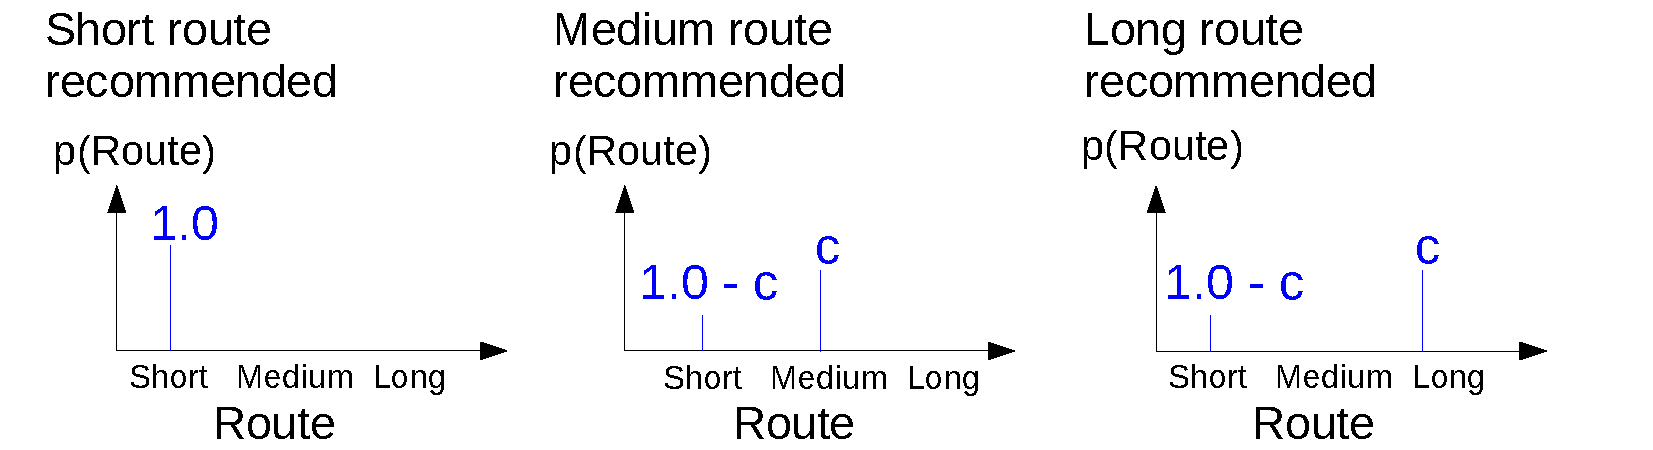
\includegraphics[width=0.85\textwidth]{../figures/investigation/VergleichUmleitalgorithmen/modelroutechoiceprobs.pdf} 
\caption[Discrete probability distributions for different route recommendations]{Discrete probability distributions for different route recommendations.  The default behavior is to take the short route which is why the probability assigned is 1.0 (left). The discrete probability distribution is controlled through the parameter compliance rate c (middle, right). }
\label{fig:distsforparameter}
\end{figure}


The novel cognition model is implemented as \textit{ProbabilisticCognitionModel} class in  \textit{Vadere}. At each time step, the update method is called which checks whether an agent has already received the route recommendation. If the information is new, the agents makes a route choice which is realized by choosing one of the intermediate targets placed at each route. The target is randomly drawn from a discrete probability distribution, see Listing~\ref{lst:drawnewtarget}.  

%public void update(Collection<Pedestrian> pedestrians) {
%   for (Pedestrian p : pedestrians) {
%       Stimulus stimulus = p.getMostImportantStimulus();  
%       if (stimulus instanceof InformationStimulus) {
%          InformationStimulus info = p.getMostImportantStimulus();
%          ...
%          if (p.getKnowledgeBase().getKnowledge().size() == 0) {
%               LinkedList<Integer> newTarget = getNewTarget(...);
%               ...
%          }  
%...}         
%
%\end{lstlisting}

\begin{lstlisting}[caption={getNewTarget() method of the novel ProbabilisticCognitionModel. Route choice is realized by drawing from a random distribution. The discrete distributions in dependency of the compliance rate are depicted in Fig.~\ref{fig:distsforparameter}. },language=java,label=lst:drawnewtarget]
public LinkedList<Integer> getNewTarget(...) {
   ...
   EnumeratedIntegerDistribution dist = new EnumeratedIntegerDistribution(..., targetIds, probabilities);
   Integer newTargetId = dist.sample();
   LinkedList<Integer> newTarget = new LinkedList<>();
   return newTarget.add(newTargetId);
}
\end{lstlisting}






\subsection{Design of the simulation study}



\subsubsection{Parameter selection and quantities of interest}


In the absence of more information, I assume the parameter \textit{compliance rate} to be uniformly distributed. The lower bound is 0 (agents always ignore instructions), and the upper bound is 1 (agents always comply with route recommendations). A compliance rate $c=0$ is similar to a setting without guidance. For each route recommendation algorithm the compliance rate is varied from 0\,\% to 100\,\%. The design of the simulation study is depicted in Fig.~\ref{fig:doeS2}. 

\begin{figure}[hbt!]
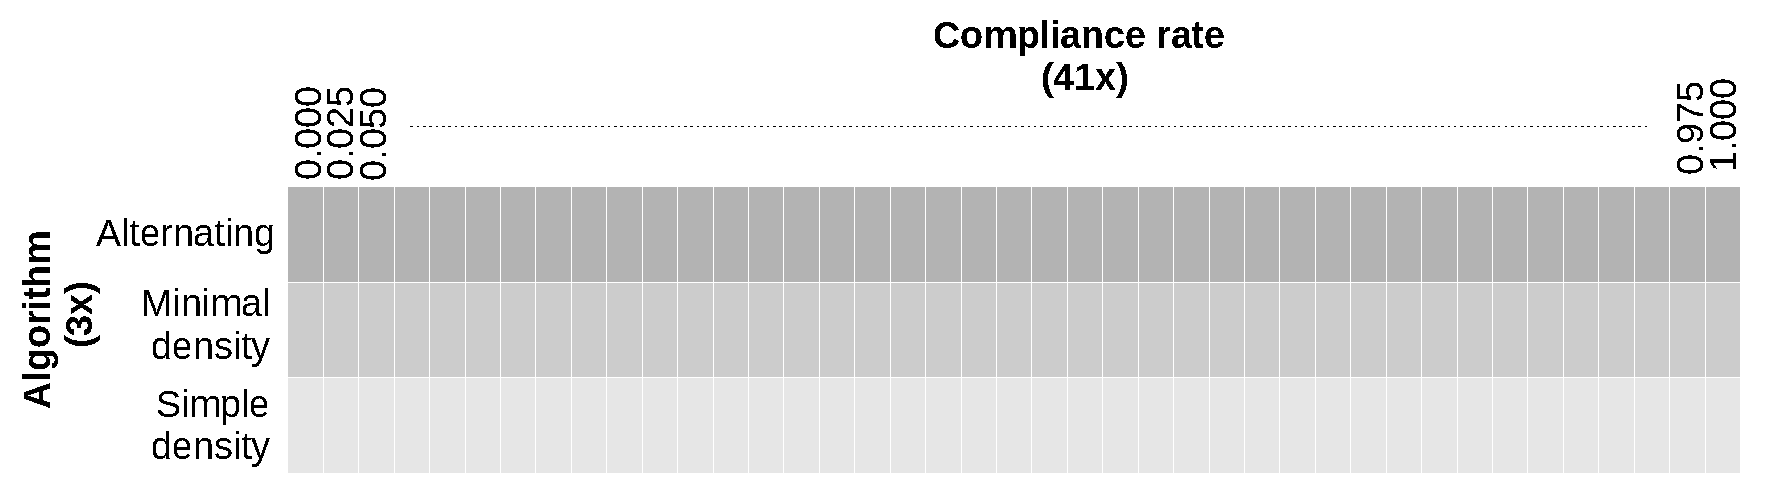
\includegraphics[width=\textwidth]{../figures/investigation/VergleichUmleitalgorithmen/designSimStudy.pdf} 
\caption[Design of the algorithm selection study]{Design of the simulation study. For each route recommendation algorithm, the compliance rate is varied between 0 and 1. 41 discrete compliance rates are tested.}
\label{fig:doeS2}
\end{figure}



To compare the performance of the algorithms the densities are measured in each of the three corridors, see Fig.~\ref{fig:designumleitalg}. To detect congestion,  velocities are measured. To understand the effect on the travel comfort, the individual travel time, that is the time an agent needs to walk from the source to a target, is recorded. See Tab.~\ref{tab:doe} for an overview of quantities of interest.
The quantities of interest are measured every $0.4\,\text{s}$, that is, the default time step size of the \textit{Vadere} simulator. For estimating the density, the classical method is used where the density is the number of agents divided by the measurement area: $d = N/A$.
As velocity, the spatial mean velocity is used  which is defined as the average of the pedestrians’ individual velocities within a measurement area.
% 

 

%


%



\begin{table}[H]
\center
\begin{tabular}{ll}
\hline
Quantities of interest & Unit  \\  \hline
Individual travel time  & $s$ \\
Density (for each corridor) & $ped/m^2$ \\                                                                             Velocity (for each corridor) & $m/s$ \\ \hline
\end{tabular}
\caption[Quantities of interest of the algorithm selection study]{Quantities of interest of the route recommendation algorithm study. The densities and velocities are measured in the three measurement areas (red areas in Fig.~\ref{fig:designumleitalg}) every 0.4\,s. For each agent, the individual travel time is recorded. }
\label{tab:doe}
\end{table}

The simulation study is carried out using the \textit{SUQ-controller} module of \textit{CrowNet}. To reduce the total simulation time, 10 simulations are run in parallel. The study is run on a server that is described in Appendix~\ref{sec:VirtualMachine}.


\subsubsection{Expected minimum compliance rate from flow equations}
I estimate the minimum compliance rate that is necessary to resolve congestion to check the plausibility of the simulation results. For this purpose I use the jamming criterion from Section~\ref{sec:fundamentaldiagram}. As a reminder, the criterion says that there is congestion when the inflow exceeds the capacity of a bottleneck. The capacity $J_C$ is the maximal pedestrian flow through the bottleneck. If $J_C$ is the upper limit, the lower limit $l$ of the percentage of people that need to be redirected, is:
\begin{equation}
l = \frac{J_{in}-J_{C}}{J_{in}}
\label{fig:jammingCrit}
\end{equation}

The inflow is $J_{in}=1.60\,\text{ped/(ms)}$ in the scenario. As capacity value I use $J_C=1.30\,\text{ped/(ms)}$. This value is in line with handbooks~\cite{weidmann-1994-cdyn,hurley-2016-cdyn} and also with the fundamental diagram that I derived from the simulation of the unguided setting, see Appendix~\ref{sec:capacityestimation}.

The alternating algorithm recommends the shortest corridor to $1/3$ of the people. Thus, a proportion of $q=2/3$ of the people are directed away from it. With a compliance rate $c$, the flow in the short corridor is:
\begin{equation}
J_{short} = J_{in}(1- c q(c))
\end{equation}
To avoid a jam, it is required that $J_{short} \leq J_C$. Thus, the minimum compliance rate is 
%to avoid congestion is
\begin{equation}
c = \frac{1}{q(c)}\left( 1- \frac{J_C}{J_{in}} \right)
\label{eq:complianceRate}
\end{equation}
Plugging $q=2/3$ into Eq.~\ref{eq:complianceRate} yields a compliance rate of at least $28\%$ to avoid congestion. 
%
For two density-based route recommendation algorithms, $q(c)$ depends on the flow situation.  Therefore, one cannot estimate a minimum compliance rate in advance.



\subsection{Effect of guiding strategies}



\subsubsection{Congested routes cause high travel times}

I first look at the case without guidance where all agents take the short route, see Fig.~\ref{Fig4}. For the performance evaluation, only the steady state of the system is considered, which is reached when densities and velocities stagnate. A steady-state flow has been reached  after about $250\,$s, see Fig.~\ref{Fig5}.  Measurements taken before $250\,$s are excluded from the following analysis.


\begin{figure}[hbt!]
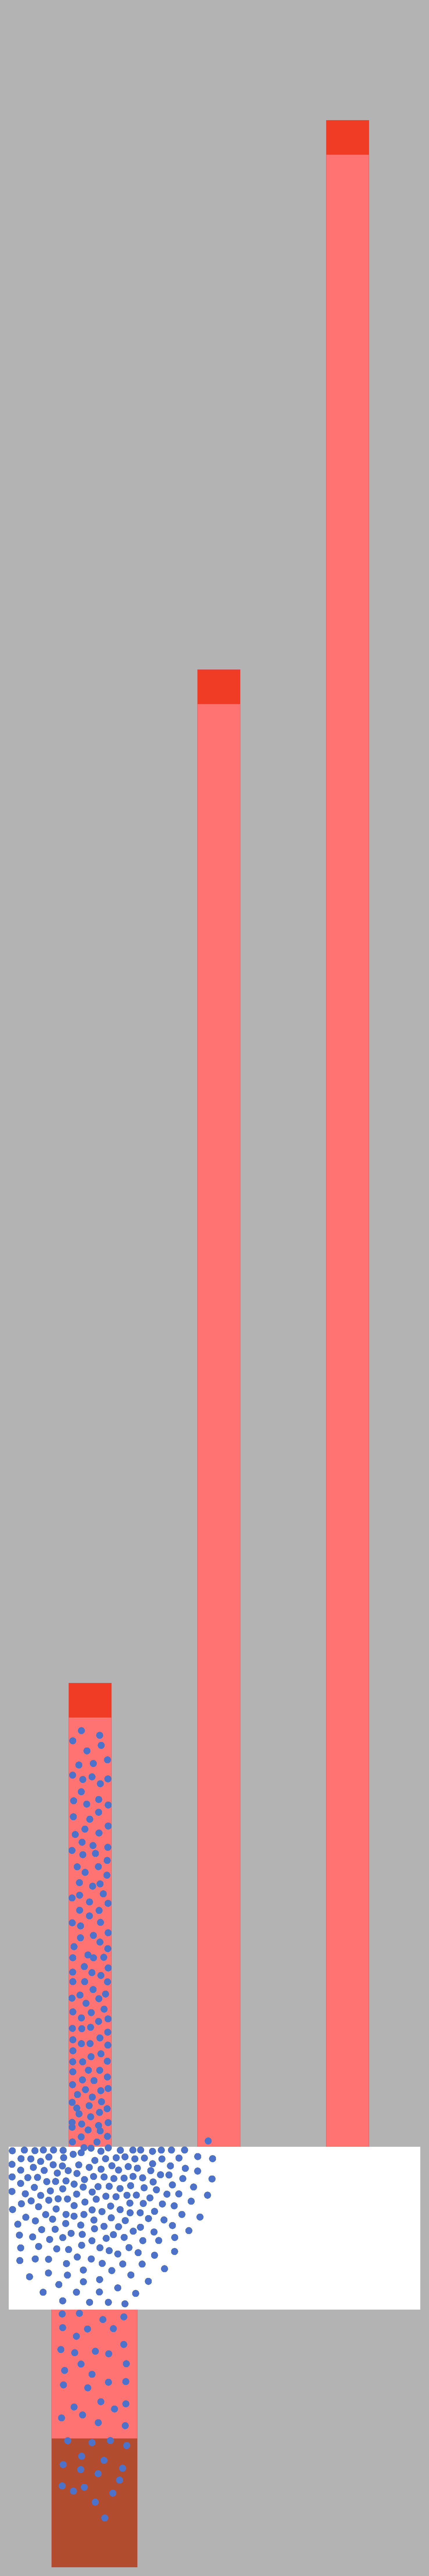
\includegraphics[angle=270,width=14.5cm]{./investigation/crownetOutput/guiding_strategies/tikz/guiding_no_controller_250s.pdf} 
\caption[Setting without guidance]{Setting without guidance. All agents take the short route (simulation time $t=250\,$s). Congestion occurs because the inflow is larger than the capacity of the short corridor.}
\label{Fig4}
\end{figure}



\begin{figure}[hbt!] 
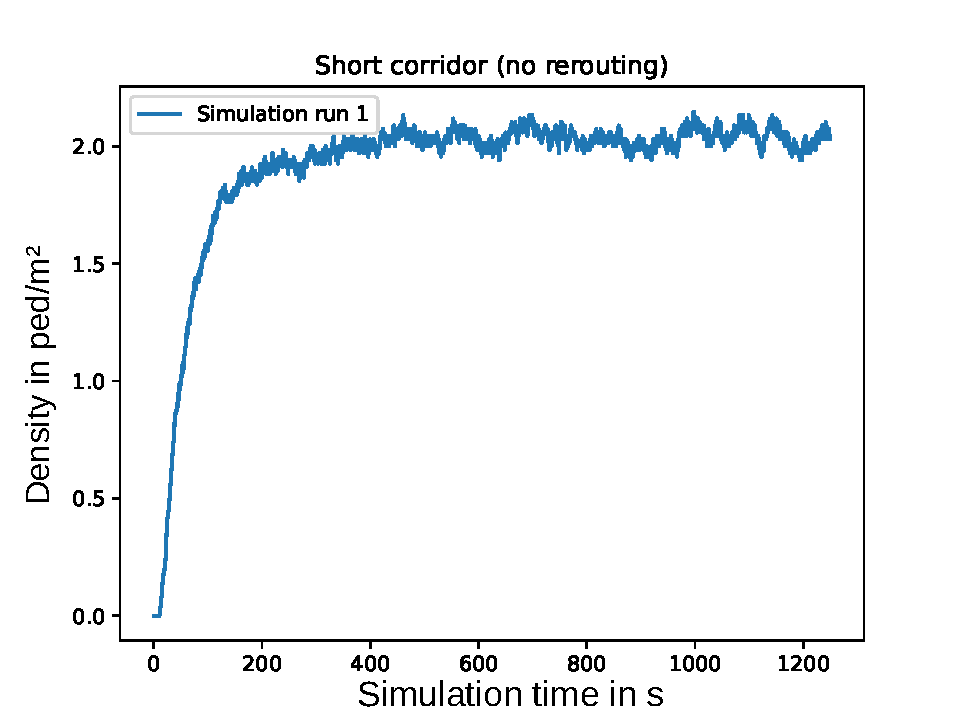
\includegraphics[width=0.5\textwidth]{./investigation/crownetOutput/guiding_strategies/DensityOverTime.pdf} 
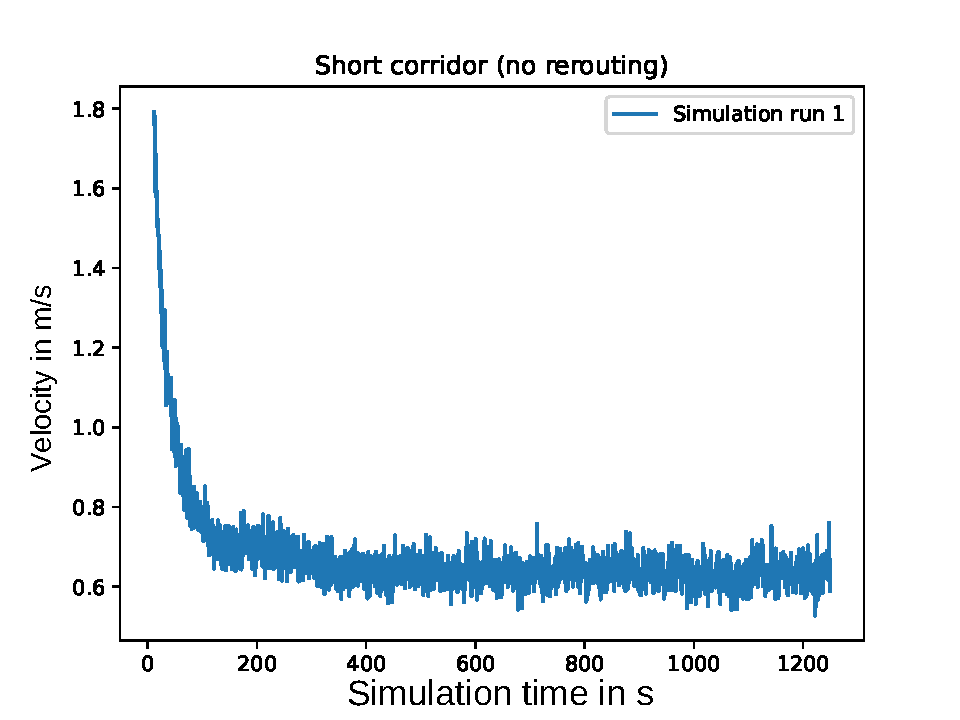
\includegraphics[width=0.5\textwidth]{./investigation/crownetOutput/guiding_strategies/VelocityOverTime.pdf} 
\caption[Velocity and density in the short corridor]{Velocity and density in the short corridor over the simulation time in the setting without guidance. 
A steady-state flow is reached at approximately $250$\,s. Densities and velocities before $250\,$s are not included in the evaluations. }
\label{Fig5}
\end{figure}

Tab.~\ref{tab:velocitiesDensities} lists the measured values on the short route:
%
For the density and the velocity, the median and the mean values are identical. However, the mean travel time is considerably lower than the median travel time. Since this indicates that the travel time does not follow a normal distribution the median travel time is used for further evaluations. 
%

The short route is approximately 50\,m long. With a mean free-flow velocity of 1.34\,m/s, the default parameter of the locomotion model, one would expect an average travel time of around 37\,s, if agents walked freely. Instead, one observes congestion in the short corridor 
at a mean density of $2.0\,\text{ped}/\text{m}^{2}$ and with a walking speed reduced to $0.65\,\text{m/s}$ on average. 
% 
The density value of $2.0\,\text{ped}/\text{m}^{2}$ corresponds to E as a level of service according to Fruin. The movement temporally stops and no passing maneuvers are possible. Moreover, the median travel time of $178\,$s is almost five times longer than expected in a free flow regime, see Tab.~\ref{tab:velocitiesDensities}. 
%
%Furthermore, the jamming criterion is fulfilled. The capacity of the short corridor is between $1.3 ped/(ms)$ and $1.54 ped/(ms)$, see supporting information (S2 Appendix). This is lower than the inflow $1.60 ped/(ms)$. Thus our results are plausible.



\begin{table}[hbt!]
\begin{footnotesize}
\centering
\begin{tabular}{lrrrrrrrr}
\toprule
 & sample size & mean & std & min & 25\% & 50\% & 75\% & max \\
\midrule
Density $ped/m^2$ & 2500 & 2.03 & 0.05 & 1.85 & 2.00 & 2.03 & 2.06 & 2.15 \\
Velocity $m/s$ & 2500 & 0.64 & 0.03 & 0.53 & 0.62 & 0.64 & 0.66 & 0.76 \\
Travel time [s] & 2783 & 191.32 & 80.76 & 66.80 & 142.80 & 176.80 & 210.00 & 843.60 \\
\bottomrule
\end{tabular}
\end{footnotesize}
\caption[Statistics of the short corridor for the setting without guidance]{Statistics of the short corridor for the setting without guidance. Mean values, standard deviation, median, and further statistical quantities for the density and the velocity are computed using 2500 samples.
The median and the mean value are similar for the density and the velocity. 2783 individual travel are used to compute the statistics of the travel time.
The mean travel time is considerably lower than the median travel time, indicating that it is not normally distributed. }
\label{tab:velocitiesDensities}
\end{table}



\subsubsection{Any route recommendation algorithm reduces the travel time}

Without guidance there is congestion resulting in high travel times. Fig.~\ref{fig:travelFig11} shows the 25th, 50th and 75th percentiles  of the travel time in dependency of the compliance rates. The black lines  refer to the  setting without guidance ($c=0$)
and represent an upper limit. The graphs are always below the black line, thus,
any algorithm reduces the travel times in the scenario. 

The minimum travel time is not achieved at the highest compliance rates, but at intermediate compliance rates. In Fig.~\ref{fig:travelFig11} (middle), one can observe that the median travel time is around 100\,s for the \textit{minimal density algorithm} at full compliance ($c=1.0$). The minimal median travel time (60\,s) is achieved when the compliance rate is $c \in [0.2,0.5]$ for the \textit{minimal density algorithm} and $c \in [0.3,0.8]$ for the \textit{alternating algorithm}. For the \textit{simple density algorithm}, the median values become minimum for $c \in [0.2,1.0]$.
The reason for this behavior is that full compliance evens out densities, but it does not optimize travel times. 
Imagine a compliance rate of $c=0.3$. In this case, at least 70\,\% ($ 70\%=1-c$) of the agents take the short corridor. Thanks to sufficiently many other agents taking longer routes, there may be elevated density on the short path, but no congestion. This means short travel times for most. 
%
On the other hand, if 100\% of the agents reject the route recommendation, the setting 
is equivalent to the scenario without guidance where the travel time peaks, see Fig.~\ref{fig:travelFig11}. This explains the rapid fall of the 25th, 50th and 75th percentiles of the travel time when $c \in [0.0,0.2]$. 

As soon as congestion is resolved, agents who take a longer route will reach the destination later. In the scenario, more than 75\,\% of the agents still reach their target faster than in the default setting with congestion, see~Fig~\ref{fig:travelFig11} (right): the 75th percentile is always below the black line. Interestingly, the 75th percentiles differ strongly for the three algorithms if the compliance rate is $c> 0.2$. The 75th percentiles of the density-based algorithms are always higher than the 75th percentiles of the alternating algorithm, see again~Fig~\ref{fig:travelFig11} (right). This is caused by the fact that the two density-based algorithms recommend the long route more often than the \textit{alternating algorithm}. Therefore, more agents have longer walking paths.





\begin{figure}[h!]
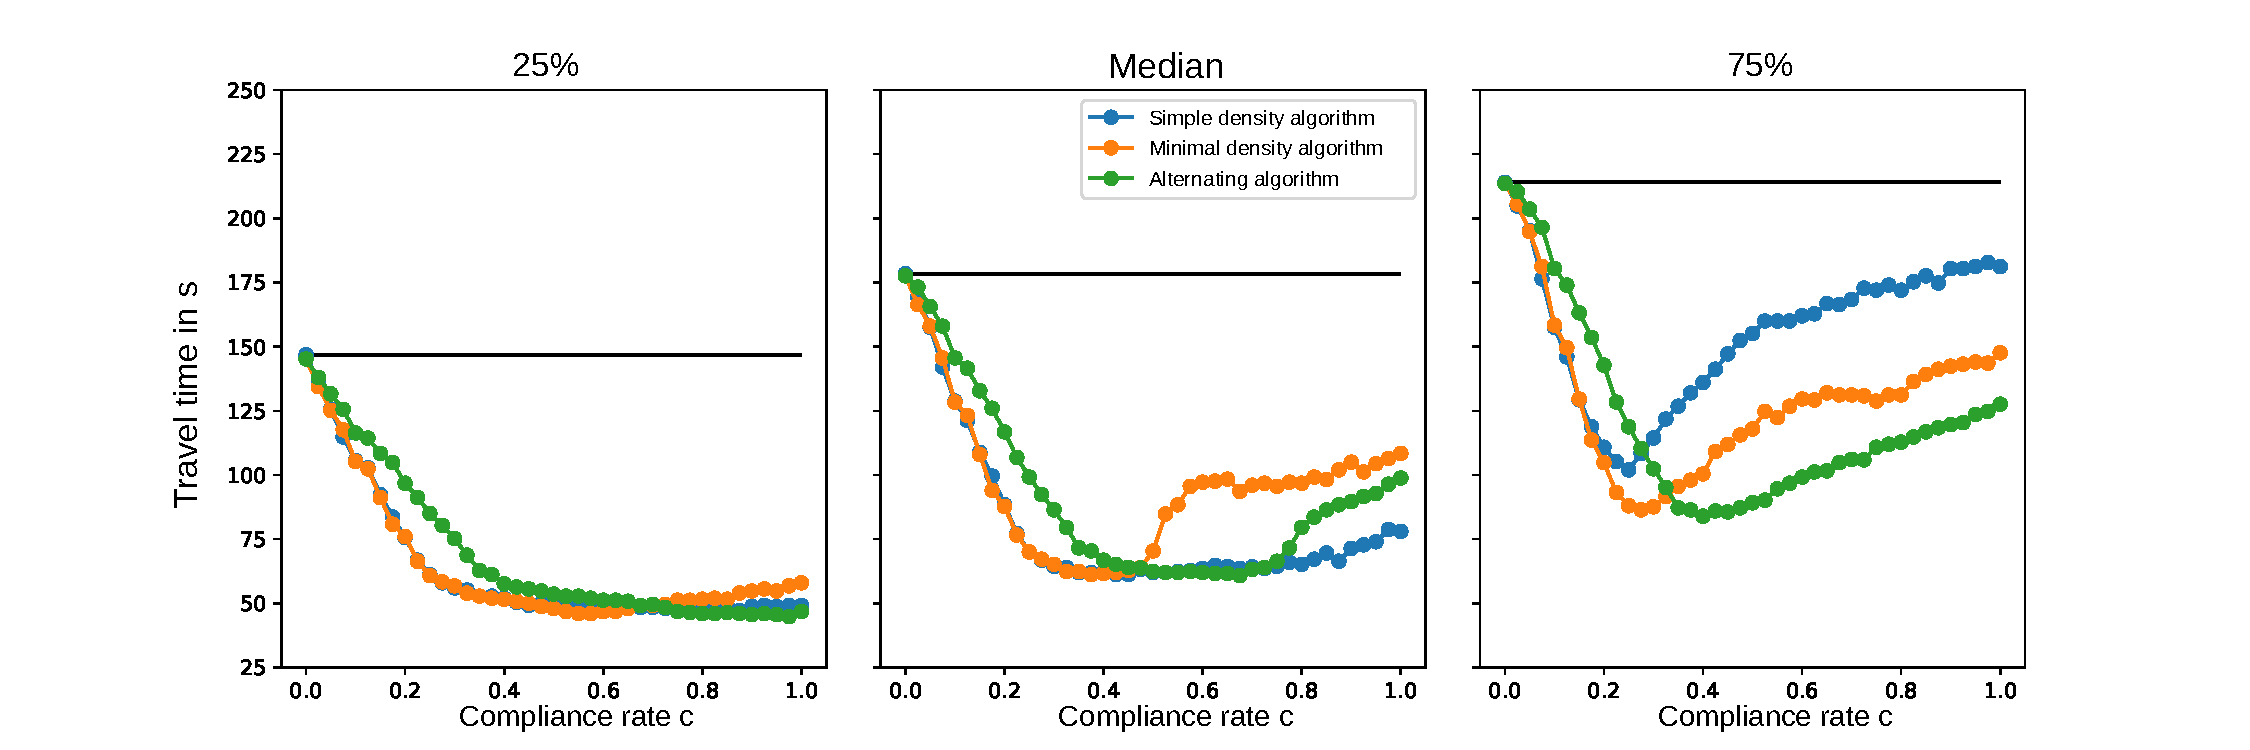
\includegraphics[width=\textwidth,trim={2.4cm 0.0cm 3cm 0.6cm},clip]{./investigation/crownetOutput/guiding_strategies/Travel_time.pdf} 
\caption[25th, 50\% and 75\%-quartiles of the travel time in dependency of the compliance rate.]{25th, 50th and 75th percentiles of the travel time in dependency on the compliance rate. The percentiles show at which compliance rate a certain percent of all agents experience travel times below the given value.
The black line represents the setting without guidance, that is, a compliance rate of $c=0$. The orange line represents the \textit{minimal density algorithm}, the blue line the \textit{simple density algorithm} and the green line the \textit{alternating algorithm}.
The three algorithms reduce the travel times for any compliance rate $c>0$: The percentiles are always below the black line (without guidance).}
\label{fig:travelFig11}
\end{figure}



\subsubsection{A small proportion of compliant people suffice to avoid jamming}

Whether or not an algorithms avoids congestion depends on the compliance rate. If no one listens to the route recommendation $(c=0)$, the situation is just as if there were no guidance. Based on the jamming criterion calculation, I estimated that congestion resolves for the \textit{alternating algorithm} if the compliance rate is $c>0.28$.
The upper third of Fig.~\ref{fig:densitiesFig6} depicts the density over the compliance rate in the short corridor. One can observe that the density increases when the compliance rate decreases. 

With compliance rates below about $c=0.3$ the density stagnates for the alternating algorithm.
This is close to the estimate of $c=0.28$. Note that the jamming criterion only evaluates congestion within the bottleneck. It does not consider agents of the bottleneck: One can observe this effect in Fig.~\ref{fig:snapshotscomparison}. However, the number of waiting agents is much lower compared to the setting without guidance. 

For the two density-based algorithms, one can observe that the densities stagnates when the compliance rate is $c\approx0.2$, see Fig.~\ref{fig:densitiesFig6} (top left and top center). 
%Thus, compared to the alternating algorithm, a lower compliance rate suffices to resolve congestion.



\begin{figure}[H]
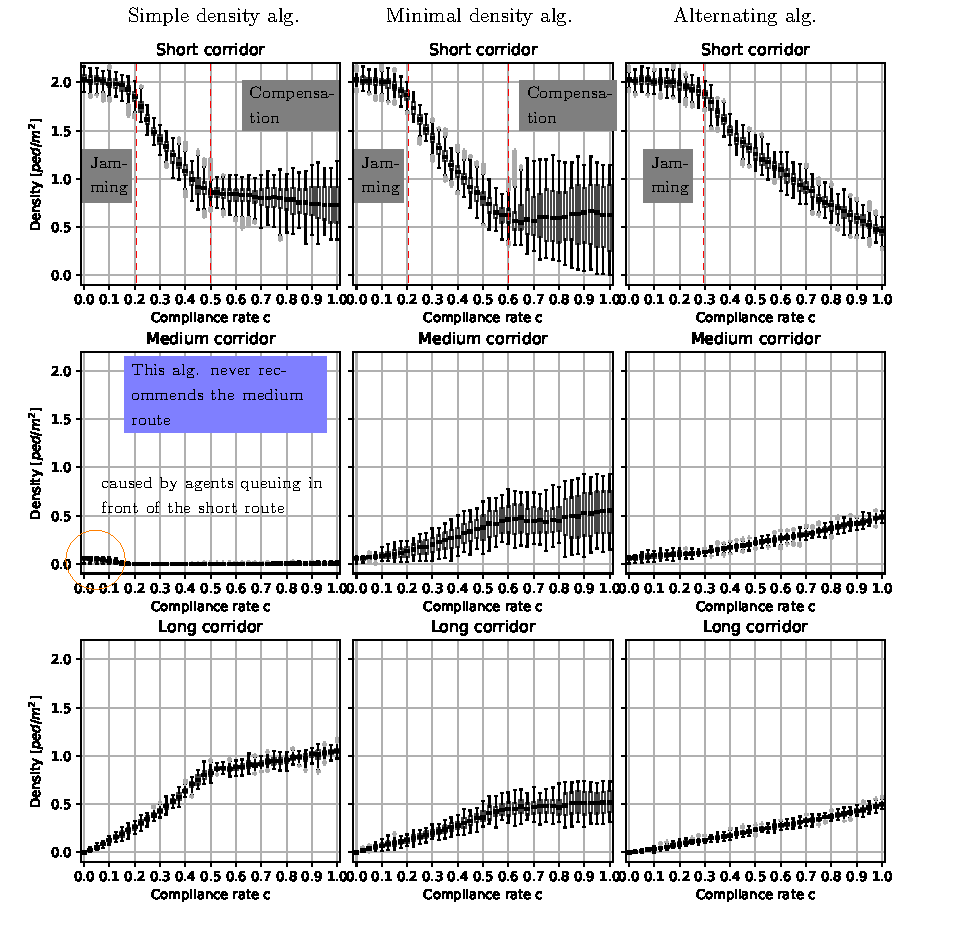
\includegraphics[width=1.1\textwidth]{../figures/investigation/VergleichUmleitalgorithmen/densities_tikz.pdf} 
\caption[Boxplots of the densities per route ]{Boxplots of the densities per route.
The boxes represent the 25th and 75th percentiles. The thick black line in a box indicates the median value. Whiskers do not extend up and down from the box more than $1.5$ times the interquartile range (75th percentile - 25th percentile). Values outside the whiskers are considered as outliers (gray dots). Different states can be observed: If the compliance rate is small, jamming occurs. With better compliance, the density decreases. Both density-based algorithms can compensate the lack of compliance: the density hardly changes for $c>0.5$ and $c>0.6$ respectively (top: left and center). The \textit{alternating algorithm} cannot fully compensate a lack of compliance (top: right).}
\label{fig:densitiesFig6}
\end{figure}


\begin{figure}[H]
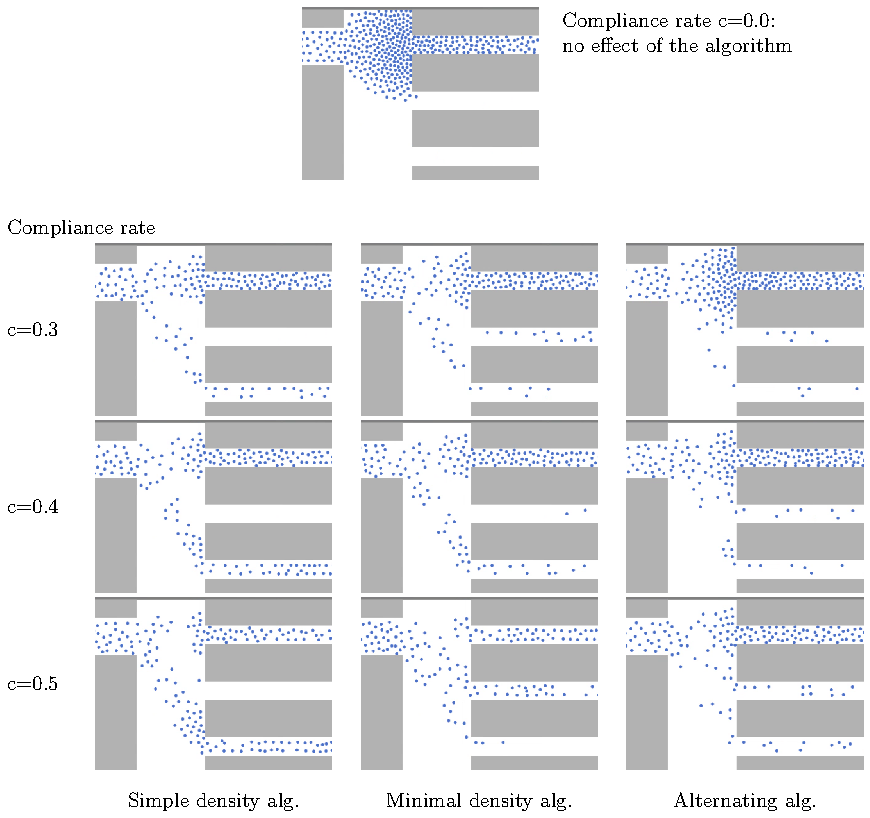
\includegraphics[width=\textwidth]{../figures/investigation/VergleichUmleitalgorithmen/snapshots/snapshotscollected.pdf} 
\caption{ Simulation snapshots at simulation time $t=300$\,s. The congestion in front of the bottleneck dissolves with increasing compliance rate. With the density-based algorithms, the congestion is almost completely resolved at a compliance rate $c=0.3$. With the \textit{alternating algorithm}, the congestion is resolved at a higher compliance rate ($c=0.4$) because this algorithm cannot respond to the current density situation.
}
\label{fig:snapshotscomparison}
\end{figure}

Next I analyze which routes are recommended at certain compliance rates. The \textit{minimal density algorithm} never recommends the short route when the compliance rate is low: $c<0.575$. 
The \textit{simple density algorithm} recommends the long route all the time when the compliance is $c<0.425$. Therefore, the proportion of people directed away from the short route is in both cases $q=1$. Now that $q=1$ is known, the minimum compliance rates can be estimated according to  Eq.~\ref{eq:complianceRate} for the two density-based algorithms. The resulting minimum compliance rate is $c=0.19$ . This is line with the density situation, see Fig.~\ref{fig:densitiesFig6} (top left and top center). The density behavior changes for both algorithms at $c\approx0.2$. 
Interestingly, the median travel time becomes minimal as soon as congestion is resolved, see Fig.~\ref{fig:travelFig11}. This is true for any scenario where the waiting time caused by congestion is longer than the time required to take a longer alternative route. Importantly, it shows that resolving congestion not only improves safety but can also improve travel service by reducing travel times.

An important finding is that the two density-based algorithms can compensate missing compliance better than the \textit{alternating algorithm}, see again Fig.~\ref{fig:densitiesFig6} (top left and top center). 
The lower the compliance rate, the more non-compliant agents congregate in the short corridor
so that the density-based route recommendation algorithms favor alternative routes. Thus, congestion is resolved at lower compliance rates, see again Fig.~\ref{fig:snapshotscomparison}. Note that for any algorithm, the non-compliant agents remain in the short corridor where the density is high. Only compliant agents enjoy a better level of service along the medium or long route.
Fig.~\ref{fig:densitiesFig6} shows that the \textit{minimal density algorithm} fully compensates the lack of compliance for compliance rates $c>0.6$: the median density is at a fixed value. For the \textit{simple density algorithm} the threshold is similar: $c=0.5$.









\subsubsection{Similar level of services for the three route recommendations}


To evaluate the safety, the maximum densities are analyzed. For all of the algorithms, the maximal density values occur on the short route, see again Fig.~\ref{fig:densitiesFig6}. The density values in the short route (top row) are higher than the density values in the medium and long route (second and bottom row) for any compliance rate.

For each algorithm, 41 simulation runs are available that refer to the 41 discrete compliance rates. For each simulation run, the maximum density is extracted. The resulting distributions are depicted as boxplots in Fig.~\ref{fig:maxdensitiesroutere}. One can observe that the \textit{alternating algorithm} achieves services levels according to Fruin that range from C ($<0.72\,\text{ped/m}^2$) to E ($<2.17\,\text{ped/m}^2$). The density-based algorithms achieve densities that correspond to the service levels D ($<1.08\,\text{ped/m}^2$) and E ($<2.17\,\text{ped/m}^2$).
The spread is large because the compliance rate has a strong influence, see again~Fig.~\ref{fig:densitiesFig6}.




\begin{figure}[hbt!]
\centering
\begin{tikzpicture}
\node[] at (0,0) {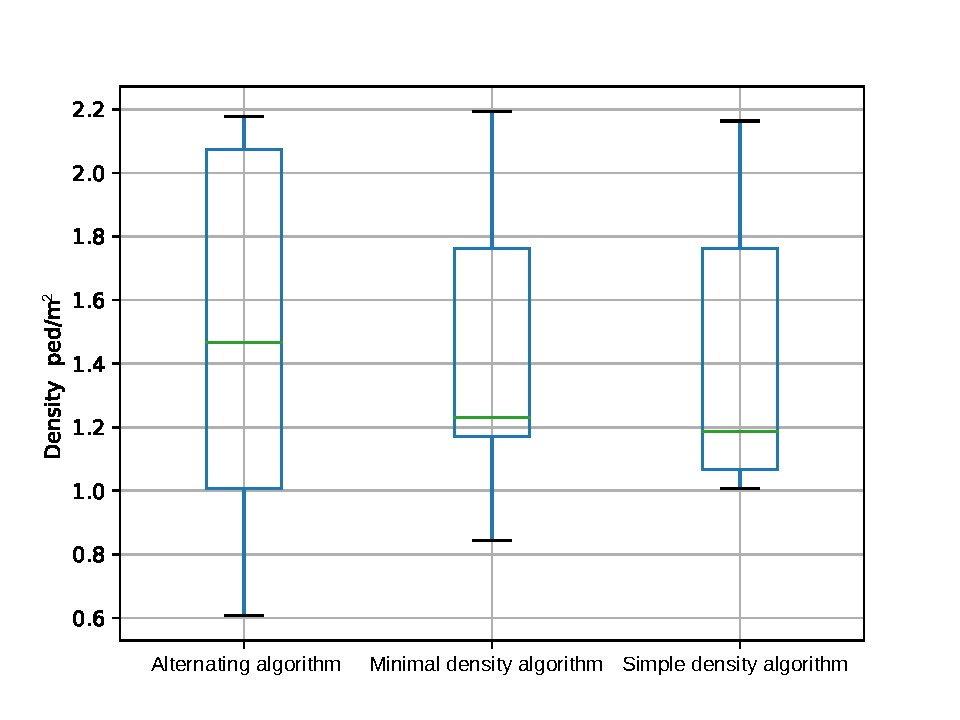
\includegraphics[width=0.8\textwidth]{./investigation/crownetOutput/guiding_strategies/maxDensitities.pdf}};
\draw[dashed] (-4.2,3) -- (8,3);
\draw[dashed] (-4.2,-2.7) -- (8,-2.7);
\draw[dashed] (-4.2,-1.2) -- (8,-1.2);
\node[] at (7,-3.2) {Level of Service C};
\node[] at (7,1) {Level of Service E};
\node[] at (7,-2) {Level of Service D};


\end{tikzpicture}
\caption[Boxplots of the maximal densities]{Boxplots of the maximum densities. For each route recommendation, I extracted the maximal density from each of 41 simulation runs that differ in their compliance rate. A Kruskal Wallis test reveals that the medians (green line) do not differ statistically.}
\label{fig:maxdensitiesroutere}
\end{figure}


In order to test whether one of the algorithms leads to lower maximum densities and, thus, to better safety, the maximum densities are compared statistically. First, the distributions are tested for normality. KS-tests reveal that the three distributions are not normally distributed (\textit{Alternating algorithm}: $D=0.985$, p-value\,$=0.000$, \textit{Minimal density algorithm}: $D=0.986$, p-value\,$=0.000$, \textit{Simple density algorithm}: $D=0.985$, p-value\,$=0.000$). 

Because the distributions are not normally distributed a Kruskal Wallis test is used to test whether the median values of the maximum densities differ. Since the p-value is larger than the significance level of 0.05 ($H=1.010$, p-value\,$=0.603$), I cannot reject the null hypothesis that the median density is the same for all three algorithms. Thus, I do not have sufficient proof to claim that different route recommendation algorithms lead to statistically significant density differences. I conclude that there is no superior route recommendation algorithm that outperforms the others. All three route recommendation reduce congestion similarly successful.



\subsubsection{The simple density algorithm requires few redirection measures}

Finally, I look a the number of route recommendations generated by the three algorithms. I assume that an algorithm is more likely to be implemented in practice when it requires only a low number of interventions in the system. Also, I expect that the acceptance of the crowd guidance system is higher when people do not receive redirection instruction permanently.
According to their definition, the \textit{alternating algorithm} and the \textit{minimal density algorithm} generate a route recommendation every 2\,s. The \textit{simple density algorithm} only generates a route recommendation when the short route is more occupied than the long route.  In the scenario, the \textit{simple density algorithm} intervenes the system less often than the other algorithms, see Fig~\ref{fig:numberofRouteRecs}. One could argue that the number of recommendations is similarly low for the \textit{alternating algorithm} if the short default route was not recommended. This is true, but the algorithm cannot resolve congestion at a low compliance rate. I conclude that the \textit{simple density algorithm} has the best cost-benefit ratio: It resolves congestion successfully, while the crowd is only redirected if necessary.




\begin{figure}[hbt!]
\centering
\begin{tikzpicture}[scale=0.94, transform shape]
\node[] at (0,0) {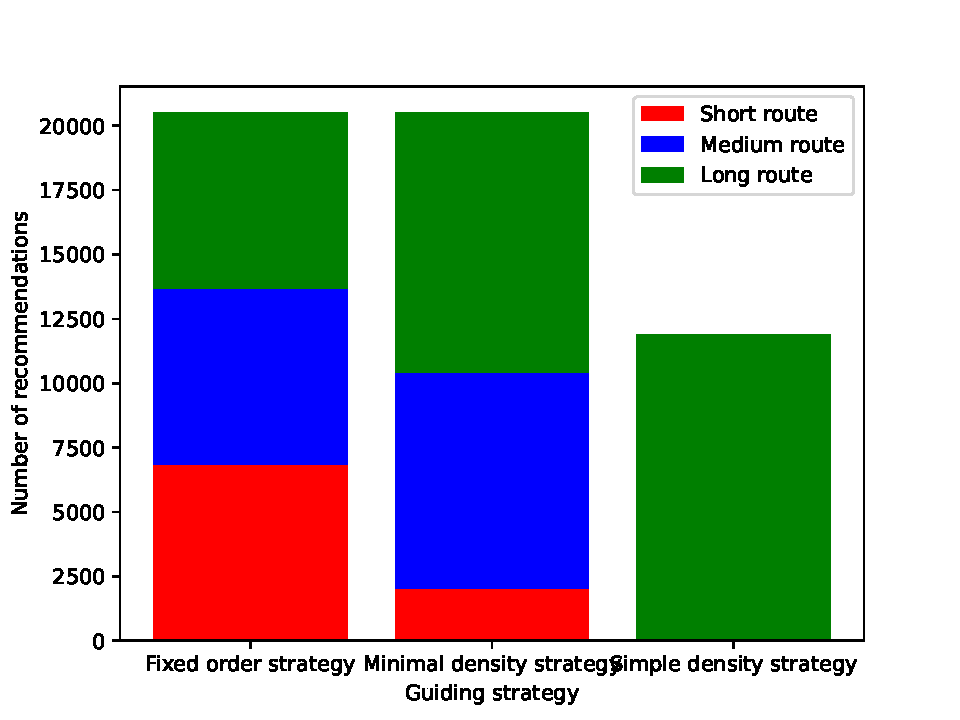
\includegraphics[width=12cm,trim={0cm 1.15cm 0cm 0cm},clip]{./investigation/crownetOutput/guiding_strategies/NumberOfRouteRecommendations.pdf}};
\node[text width=2.5cm] at (-2.5,-4.8) {Alternating alg. };
\node[text width=2.5cm] at (0.1,-4.8) {Minimal density alg. };
\node[text width=2.5cm] at (3.5,-4.8) {Simple density alg. };
\end{tikzpicture}
\caption[Number of route recommendations]{Number of route recommendations. Each algorithm is evaluated 20500 times (= 500 route recommendations x 41 compliance rates) 
The \textit{alternating algorithm} recommends every route equally often according to its definition (left). The \textit{minimal density algorithm} recommends the short route less often to resolve congestion (middle). The \textit{simple density algorithm} only recommends the long route when necessary.  }
\label{fig:numberofRouteRecs}
\end{figure}

\FloatBarrier


\subsection{Summary, limitations, lessons learned}

\subsubsection{Summary of the study}
In this section I tested how suitable route recommendation algorithms are for resolving congestion when the proportion of pedestrians complying with route recommendations is uncertain. Since I could not find suitable algorithms in my literature review I proposed three algorithms myself: 
The first algorithm sequentially directs pedestrians to different routes. The second algorithm redirects pedestrians the route with the lowest density. 
In the third algorithm, pedestrians are directed away from the congested route if the density here is higher than on the longest  alternative route. To test the algorithms, I modeled a simple topography with three routes of different lengths and similar corridor widths. In a parameter study the compliance rate, that is the proportion of pedestrians that comply with route recommendations, was varied between 0\,\% and 100\,\%. The results showed that density based algorithms resolve congestion at lower compliance rates than the alternating algorithm that does not consider the current density situation. I found that all of the algorithms lead to a reduction of the travel time in my scenario. Interestingly, the travel time was not minimal at high compliance rates since the algorithms consider densities but do not optimize travel times. 
To evaluate safety, I analyzed the density situation. I found that the maximum densities do not differ statistically: All algorithms successfully resolved congestion. For this reason, I looked at the number of redirection measures. The simple density-based algorithm, which only recommends the long alternative route but not the medium route, required fewer redirection measures than the other algorithms while resolving congestion at a low compliance rate. Therefore, I concluded that this density-based algorithm is most suitable for redirecting pedestrians. 

\begin{tcolorbox}[title={Which algorithms are suitable for generating route recommendations for crowds, given not all people follow instructions? (RQ-2)}]
A density-based route recommendation algorithm can sufficiently avoid or resolve congestion by recommending the longest available alternative route if and only if the pedestrian density on this route is lower than on the congested route.
\end{tcolorbox}


\subsubsection{Limitations and future directions}

I would like to point out some limitations of the study.

The proposed algorithms are based on simple heuristics. They cannot guarantee that pedestrians will be distributed along the routes in the most effective way.

In the study, a fixed inflow rate was assumed. Therefore, the minimum compliance rate, that is, the proportion of people who need to comply with the route recommendation to resolve congestion, is specific to this scenario. 

The study assumed that people are evenly distributed within a route. In a real scenario, twists and turns create bottlenecks which lead to density differences along the route. Strategies must be found to ensure that local safety-critical congestion is not overlooked. I will propose a procedure in Section~\ref{sec:realistiscscenario}.

In the study, it was assumed that the density information and the route recommendations are immediately available and perfectly precise. If the crowd is sensed and informed using direct communication technologies, delays, and measurement errors may affect the capability of an algorithm to distribute pedestrians. This requires further investigation. I will investigate this in Section~\ref{sec:realistiscscenario}.





\subsubsection{Lessons learned for my further investigations}

The study demonstrated that heuristic route recommendation algorithms can indeed resolve safety-critical congestion. Heuristics that redirect people to less frequented routes based on crowd density measurements proved to be particularly effective. They resolved congestion even if only a small proportion of people followed the route recommendation by directing them away from the congested route sufficiently often. 

One algorithm proved to be particularly suitable because it required only a few redirection measures, while it was capable of resolving congestion even at a low compliance rate. The algorithm recommends the longest available route if and only if the pedestrian density on this route is lower than on the congested route. Therefore I suggest to use this algorithm in a crowd guidance system.




\section{Designing mobile messages for redirecting crowds}


\label{sec:reaction}
In this section, I investigate my third research sub-question (\hyperref[reserachquestions]{RQ-3}), that is, how mobile messages should be designed to improve the compliance of crowd members to follow route recommendations.
The study is inspired by a real-life  use case in Munich (Germany) where football fans need to be guided from the bus or tram to the metro. Before and after football matches, the short direct route is usually congested although there are alternative routes available. To alleviate the congestion, I suggest to use a mobile application which works according to the route recommendation algorithm that I found was most suitable (see the previous section): The long alternative is recommended if and only if the short route is congested. 

The more people follow the route recommendation, the better congestion is avoided or resolved. This is why communication plays a crucial role in a crowd guidance system. A crowd guidance system will not have any effect, when the information does not appeal to crowd members. From the social identity approach, it is known, that  peoples' response is influenced by their social identity.
Therefore, it is likely that the route choice of football fans at a train station indeed depends on their social identity.
While conventional navigation applications are designed to fulfill the needs of individuals only, the focus of this study is on the message design in a navigation app for crowd members who share a social identity. In particular, I ask:
\begin{itemize}
\item How do appeals to the social identity improve crowd members' compliance to route instructions?
\item Which other elements are necessary in a mobile message to convince crowd members? 
\end{itemize}
Due to its interdisciplinary character, the study was developed in collaboration with a crowd psychologist, see Appendix~\ref{sec:availability}. The results of the study were published in the journal article \textit{Designing mobile application messages to impact route choice}~\cite{mayr-2023-cdyn}. Therefore, this section contains textual overlaps with the publication. 
 % The reader should be aware that the results of the online study are qualitative, i.e. whether or not a message design influences route choice behavior.At the end of this section, I will look how quantitative results could be derived.



\subsection{Application scenario at metro station Münchner Freiheit}
\label{sec:applicationscenariodescription}

At the metro station M\"{u}nchner Freiheit in Munich  travelers typically take the shortest route to get from the bus station to the trains. Especially near escalators and elevators this leads to jamming and poses a safety risk, so that traffic managers are looking for ways to nudge the fans towards alternative, but longer routes. 
In total, there are three routes of different lengths to get from the bus or tram to the metro, see Fig.~\ref{fig:mapviewmuc}. 


\begin{figure}[hbt!]
\centering
\includegraphics[width=0.85\textwidth]{../figures/investigation/Nachrichtengestaltung/scenario.pdf} 
\caption[Application scenario of the online survey]{Application scenario of the online survey. At the train station Münchner Freiheit in Munich (Germany), three routes lead to the underground trains. Note that the map is rotated counter-clockwise (North points to the left). Footballs fans walk from the bus or tram to the underground train. The pictures depict football fans' field of vision at the different routes. The sign to the underground (big blue U) is only visible for the short route (red).  }
\label{fig:mapviewmuc}
\end{figure}

The big blue letter \textbf{U} represents an entrance to the intermediate level where all pedestrian streams come together and from which pedestrians access the underground level. To avoid crowding, fans are redirected to the long alternative route (left route marked in green) using a mobile application. Fans getting of the bus or tram can only see the U-sign pointing to the short route (picture at the bottom right). Only fans familiar with the environment are aware about the other entrance.







\subsection{Survey design: groups, information state and message design}

To test the hypothesis that football fans react differently to information than individuals due to their shared social identity, two online surveys are conducted: one with students and faculty associates at Hochschule M\"{u}nchen (Munich, Germany), and one with fans of the football team FC Bayern M\"unchen. 
For each study, the same type of messages are used, see the study design in Fig.~\ref{fig:eightcombincation}.


\begin{figure}[hbt!]
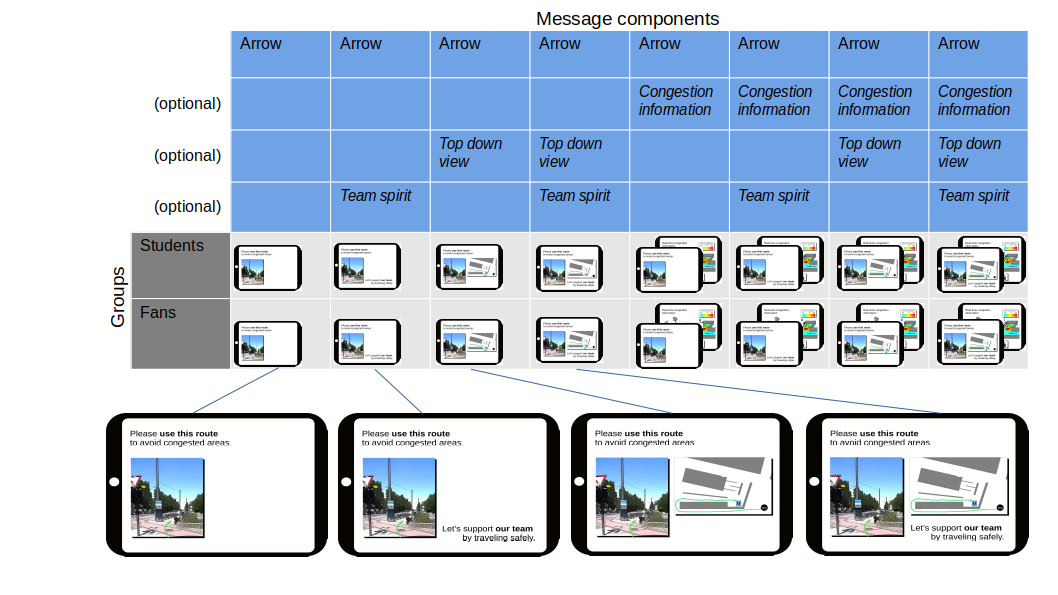
\includegraphics[width=\textwidth,trim={3.3cm 0.5cm 1cm 0.5cm},clip]{figures/investigation/Nachrichtengestaltung/design1.png}
\caption[Experimental between-subject design]{Experimental between-subject design. The eight message levels result from the combination of three optional message components: \textit{congestion information}, \textit{top down view}, and \textit{team spirit}. For a detailed view of the message components see Fig.~\ref{fig:detailviewmessagedesign}. Figure from my publication~\cite{mayr-2023-cdyn}. 
}
\label{fig:eightcombincation}
\end{figure}


The between-subjects design has one factor, message design, with eight levels. The levels stem from the combination of components. The first component is real-time \textit{congestion information} where congestion is highlighted through a color scheme. The second is a \textit{top down view} that depicts the underground train station from a top down view and with the recommended route marked in green. The third component is labeled \textit{team spirit} and refers to the motivational phrase "Let's support our team by traveling safely" (german original: "Lass uns unser Team unterstützen, indem wir sicher reisen"). The combination of these three components leads to $2^3=8$ message designs in total.  Regardless of the combination, every message 
design contains a picture with an \textit{arrow} that points in the direction of the long route and a route recommendation that is phrased as follows: `Please use this route to avoid congestion.' (german original: "Bitte benutze diese Route, um Gedränge zu vermeiden."). Fig.~\ref{fig:detailviewmessagedesign} depicts the design with all optional components. 


\begin{figure}[H]
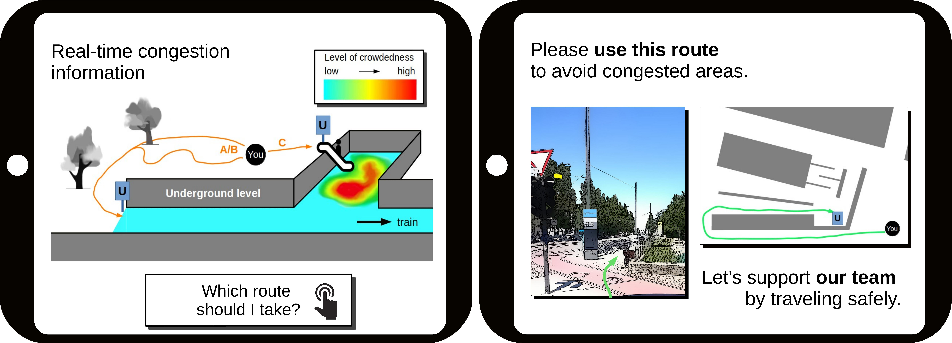
\includegraphics[width=7.3cm,clip,trim={8.1cm 0cm 0cm 0cm}]{figures/investigation/Nachrichtengestaltung/design2.pdf}
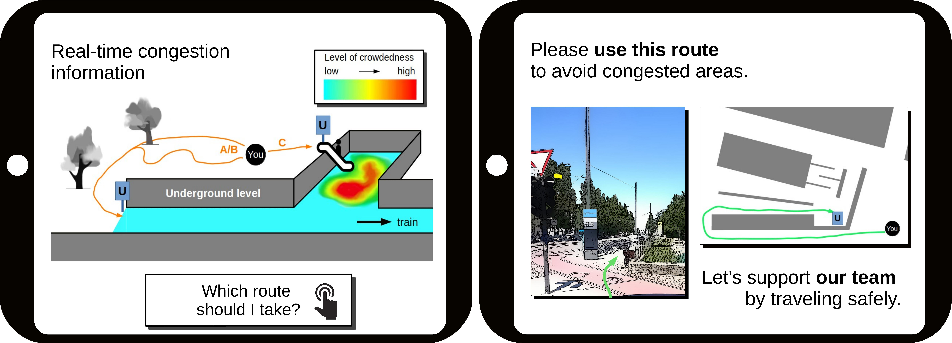
\includegraphics[width=7.3cm,clip,trim={0cm 0cm 8.1cm 0cm}]{figures/investigation/Nachrichtengestaltung/design2.pdf}
\caption[Message design with all possible message components.]{Message design with all possible message components. Left: each message design contains the sentence `Please use this route [...]' and a picture with an \textit{arrow} pointing to the entrance of the recommended route. The components \textit{top down view} and \textit{team spirit} (`Let's support [...]') are optional.  For message designs without  \textit{congestion information}, only the screen on the right is displayed to the participant.
For designs with \textit{congestion information} included, both screens are displayed. Imagine that in a real-life application, the left screen is what the app user sees first, followed by the second screen that appears when clicking on "Which route should I take?" (right). In the survey, the screens appeared next to each other. Figure from my publication~\cite{mayr-2023-cdyn}.}
\label{fig:detailviewmessagedesign}
\end{figure}



The within-subjects design has one factor, information provision, with two levels: \textit{prior to information}, and \textit{after receiving information}. To collect quantitative self-report data, a questionnaire was used.  The questionnaire is published under the doi:~\url{https://doi.org/10.1371/journal.pone.0284540.s001}. 


Maps of the scenario were depicted to participants to ensure they have similar knowledge about the surroundings, see the questionnaire. The goal was to create controlled conditions for locals and people  not familiar with the scenario. 

The dependent variables are: route attractiveness ("How likely is it that you take the following routes?"), and social identification ("I can imagine being part of the fan community."). For each, responses are scored on a 5-point Likert scale (1 = Very unlikely, 2 = Unlikely, 3 = Neutral, 4 = Likely, 5 = Very likely). The Likert-scaled estimate measures the attractiveness of each route.


\newpage
I assumed that route choice behavior changes if at least one of the three route attractiveness differs statistically when recommending the long route. I also required that not all levels increase or decrease at the same time which ensures that there is an actual change in the route choice behavior. It was always fulfilled in the study.






\subsection{Online survey with football fans and control group}
I strictly follow ethical codes for investigations with human participants. Before the online survey was launched, ethical approval was obtained from the Hochschule M\"{u}nchen University of Applied Sciences (Munich, Germany), see Appendix~\ref{sec:ethicalapproval}. Participation was voluntary and there were no monetary incentives. At the beginning of the survey, participants were informed about the research and told that their anonymised answers would be made publicly available. I also informed them that they were free to withdraw from the survey at any time. 
To participate in the survey, they had to confirm their consent and that they were at least 16 years old at the time of the participation. 


To conduct the survey, I used the free and open source online survey tool \textit{LimeSurvey}. See \url{www.limesurvey.org} for more information. Conditions were randomly assigned  to participants.
%
\textit{Students and faculty associates} were recruited through  
Facebook, the \textit{Vadere} research simulator webpage (\url{www.vadere.org}) and a general email to students and faculty associates at Hochschule M\"{u}nchen. Also, I sent personal appeals to the students of the faculty of Informatics and Mathematics at Hochschule München. 
%
Football fans are recruited using the official FC Bayern fan group on Facebook (\url{www.facebook.com/FCBFanbetreuung}) and Twitter (\url{www.twitter.com/FCBayern_FB}).

The  survey for the \textit{students and faculty associates} was conducted from 16.11.2021 to 23.02.2022. The survey for the \textit{fans} ran from 24.02.2022 to 01.03.2022.

In total, 1365 out of 3067 (44.51\,\%) participants completed the survey, while  49.12\,\% dropped out in the introductory section, before or immediately after the declaration of consent.
444 out of these 1365 participants were \textit{students or faculty associates} (43\,\% female, 54\,\% male). 921 participants were fans (18\,\% female, 80\,\% male).
Many \textit{fans} (72\,\%) were between 26 and 50 years old, see Tab.~\ref{tab1}.  \textit{Students and faculty associates} were younger: only 36\,\% fell in the range from 26 to 50, half of them were younger than 26, and 14\,\% were older than 50. 
% 


\begin{table}[ht!]
\begin{tabular}{|l|r|r|r|r|r|r|r|}
  \hline
Group & $<$18 & 18-25 & 26-35 & 36-50 & 51-65 & $>$65 & n \\ 
  \hline
Fans & 0\,\% & 17\,\% & 38\,\% & 34\,\% & 10\,\% & 1\,\% & 921 \\ \hline
  Students and faculty associates & 7\,\% & 43\,\% & 28\,\% & 8\,\% & 11\,\% & 3\,\% & 444 \\ 
   \hline
\end{tabular}
\caption[Age distribution of the two groups]{ Age distribution of the two groups: \textit{football fans} (1), and \textit{students and faculty associates} (2). \textit{Students and faculty associates} were younger than fans which might be explained by the fact that most of them were students.}
\label{tab1}
\end{table}





\subsection{Route recommendations make the long route more attractive}
%%%% Effect of information %%%%%
Prior to information, both \textit{fans} and \textit{students and faculty associates} select their routes according to path lengths. They favor the short route overall, see Fig.~\ref{fig4}. Please also find the statistical proof in Tab.~\ref{tab:surveyS2F} in Appendix~\ref{sec:collectiontables}.
The route choice changes when the long route is recommended: The long route becomes more attractive, and the short route less attractive (compare the top and bottom rows in Fig.~\ref{fig4}). The exact values are listed in Tab.~\ref{tab:surveyS2C}-\ref{tab:surveyS2D} in Appendix~\ref{sec:collectiontables}.  


As expected, Kruskal-Wallis tests reveal that the message design has a stronger effect on \textit{fans} than on \textit{students and faculty associates}. For the \textit{fans}, the message design has a significant effect on the attractiveness of the short (\textit{p}~=~$0.0000$, $H~=~95.76$, \textit{df}~=~$7$), medium (\textit{p}~=~$0.0000$, $H~=~33.04$, \textit{df}~=~$7$) and long (\textit{p}~=~$0.0022$, $H~=~22.42$, \textit{df}~=~$7$) route, while for the \textit{students and faculty associates}, the design only makes a significant difference for the short (\textit{p} = $0.0000$, $H = 45.35$, \textit{df}~=~$7$) and medium (\textit{p} = $0.0000$, $H = 32.38$, \textit{df}~=~$7$) route. The attractiveness of the long route is not affected (\textit{p} = $0.8010$, $H = 3.8113$, \textit{df}~=~$7$). An overview of the statistical results is given in Tab.~\ref{tab:surveyS2G} in Appendix~\ref{sec:collectiontables}. From this, I conclude that  \textit{fans} are more responsive to message design than \textit{students and faculty associates}.

%
Interestingly, \textit{students and faculty associates} seem to be more willing to follow route recommendations in principle because the mean attractiveness of the long route was $3.84$ for the \textit{students and faculty associates} and only $3.69$ for the \textit{fans}, see Tab.~\ref{tab2}. 

\begin{table}[ht!]
\begin{footnotesize}
\begin{tabular}{|p{8cm}|p{3cm}|p{2cm}|}
  \hline
Message design &   \multicolumn{2}{c|}{Attractiveness of long route: mean value}                                                                                                                                             \\ \cline{2-3}
 & Students and faculty associates   & Fans   \\
  \hline
  Congestion info + arrow &  3.86 (n=58) &3.50 (n=103)   \\ \hline
  Congestion info + arrow + top down view & \textbf{4.02} (n=45) & 3.90 (n=116) \\ \hline
   Congestion info + arrow + team spirit &  3.70  (n=50) & \textbf{3.98} (n=102) \\ \hline
 Congestion info + arrow + top down view + team spirit& 3.88 (n=61) &3.88 (n=107) \\ \hline
    Arrow & 3.79 (n=47) & 3.43 (n=143)  \\ \hline
   Arrow + top down view &3.94 (n=65) & 3.55 (n=111)  \\ \hline
    Arrow + team spirit  & 3.70 (n=56) & 3.55 (n=103)  \\ \hline
    Arrow + top down view + team spirit &3.82 (n=62) & 3.74 (n=136) \\ 
   \hline
 \multicolumn{1}{|r|}{ Average of means } & \multicolumn{1}{l|}{  3.84} & \multicolumn{1}{l|}{  3.69} \\
 \hline
\end{tabular}
\end{footnotesize}
\caption[Attractiveness of long route expressed through scores on a 5 point Likert scale]{
 Attractiveness of long route expressed through scores on a 5 point Likert scale.
I asked the participants how likely it is that they take the long route (1: very unlikely, 2: unlikely, ..., 5: very likely). The higher the mean value, the more attractive the long route. The message design that contains all optional components (row 4) does not achieve the highest values: 4.02, 3.98. Note that n is the sample size.}
\label{tab2}
\end{table}



\begin{figure}[hbt!]
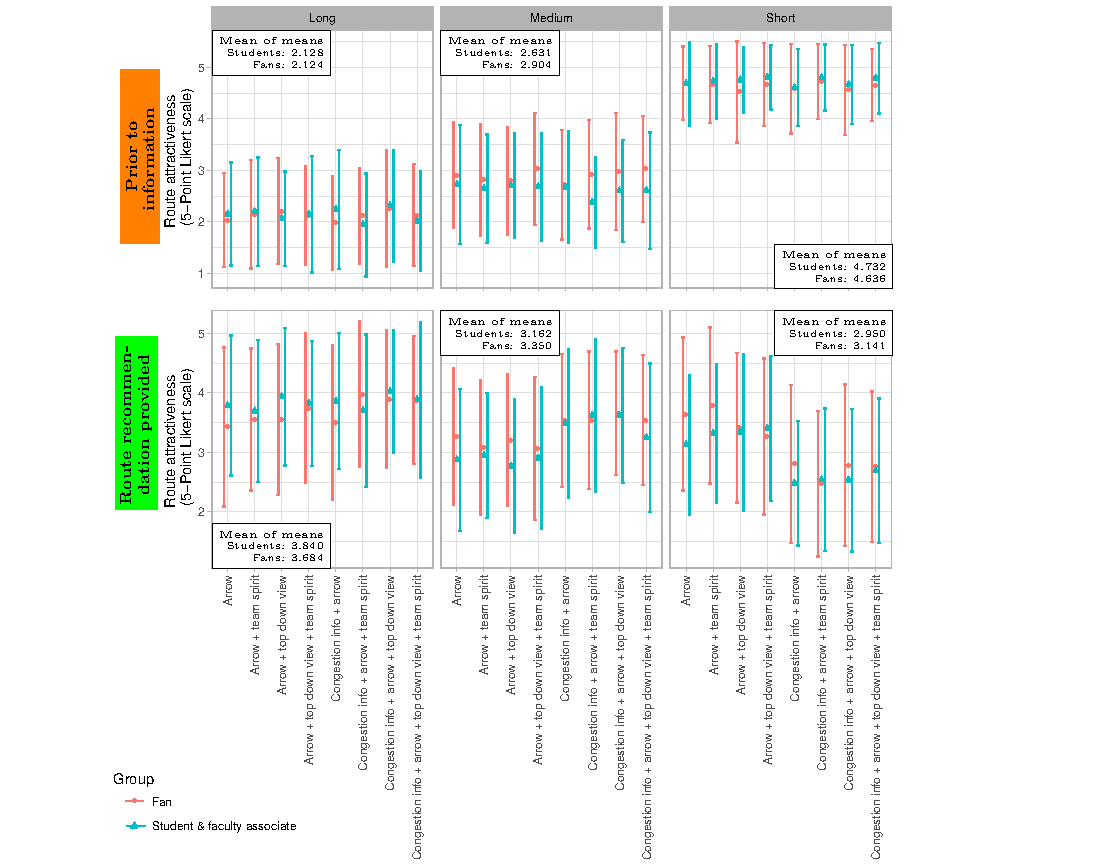
\includegraphics[width=\textwidth,trim={1.8cm 0cm 3.4cm 0cm},clip]{figures/investigation/Nachrichtengestaltung/qoI.pdf} \caption[Attractiveness of routes expressed through the Likert scale value assigned by participants]{ Attractiveness of routes expressed through the Likert scale value for each message design.  The error bars around the mean values (dots) represent the standard deviations. 
Prior to information, \textit{students and faculty associates} and \textit{fans} have a clear route preference: They favor the short route (top right) over the medium route (top center) followed by the long route (top left). With information provision, the short route becomes less attractive (bottom right) compared to the setting without information (top right), while the long route becomes more attractive (left). Figure from my publication~\cite{mayr-2023-cdyn}. }
\label{fig4}
\end{figure}

\FloatBarrier





%%%% Effect of message components %%%%
\subsection{Effect of message design on route choice}

I then conduct Mann-Whitney U tests to assess the effect of adding the message components \textit{congestion information}, \textit{top down view}, and \textit{team spirit} on the attractiveness of each route. I add one message component at each step, thus mitigating, to an extent, the inter-dependencies between designs. One can observe that adding components does not always help direct people away from the short congested route, but it never had a negative effect: 
through adding components, the short route becomes less attractive (see Tab.~\ref{tab3}, \ref{tab4}, \ref{tab:teamspirittest}) or remains equally attractive which means that the difference is statistically not significant. The non-significant results are listed in Appendix~\ref{sec:collectiontables} in Tab.~\ref{tab:surveyS2A} and \ref{tab:surveyS2B}. 

At the same time, the medium and long routes become more attractive or remain equally attractive, see again Tab.~\ref{tab3}, \ref{tab4}, \ref{tab:teamspirittest} and Tab.~\ref{tab:surveyS2A}-\ref{tab:surveyS2B} in Appendix~\ref{sec:collectiontables}. 
Crucially, adding all components together does not lead to an increased attractiveness of the long route: the mean was only 3.88 for both groups, see again Tab.~\ref{tab2}. Hence, there is evidence for an interaction between the combinations. 

There is strong evidence that the influence of the message components differs. The congestion information has always an effect on \textit{fans} and \textit{students and faculty associates}: The attractiveness of at least one route changes (see Tab.~\ref{tab3} and \ref{tab4}). 
The \textit{top down view} and \textit{team spirit} only has an effect in certain combinations with other message components. They also have a lower effect on route choice: either the short route becomes less attractive or the long route becomes more attractive. Both at the same time is never the case, see Tab.~\ref{tab:teamspirittest}.


 





\begin{table}[H]
\begin{footnotesize}
\begin{tabular}{|p{7cm}|p{2cm}|p{2cm}|p{2cm}|}
\hline
  Message design & \multicolumn{3}{c|} { Route attractiveness}                                                                                                                               \\ \cline{2-4}
  & Short route                                                                               & Medium   route                                                                            & Long route \\
\hline
Arrow                                                                             & \textit{p} = 0.0019, \newline\textit{W} = 1804.0  $\Downarrow$ & \textit{p} = 0.0117, \newline\textit{W} = 989.0   $\Uparrow$ &     \textit{not sign. \newline (\textit{p} $>$ 0.05)} \\ \hline
 Arrow + top down view                 & \textit{p} = 0.0009, \newline  \textit{W} = 1974.5  $\Downarrow$     & \textit{p} = 0.0003, \newline \textit{W} = 884.5   $\Uparrow$       &    \textit{not sign.  \newline (\textit{p} $>$ 0.05)} \\ \hline
Arrow + team spirit                   & \textit{p} = 0.0010, \newline\textit{W} = 1895.5  $\Downarrow$     & \textit{p} = 0.0031, \newline\textit{W} = 949.5  $\Uparrow$    &     \textit{not sign. \newline(\textit{p} $>$ 0.05)} \\ \hline
Arrow + top down view + team spirit &  \textit{p} = 0.0011, \newline\textit{W} = 2514.5 $\Downarrow$       &                                                                                       \textit{not sign. \newline(\textit{p} $>$ 0.05)} &  \textit{not sign. \newline (\textit{p} $>$ 0.05)} \\ \hline
\end{tabular}
\end{footnotesize}
\caption[Effect of adding congestion information to message designs on the route attractiveness]{ Effect of adding congestion information to message designs on the route attractiveness for \textit{students and faculty associates}. For each message design, I use a Mann-Whitney U test to assess whether adding \textit{congestion information} has an effect ($p<0.05$) or not.
Adding \textit{congestion information} makes the short route always significantly less attractive ($\Downarrow$). The medium route becomes significantly more attractive ($\Uparrow$) except in the case where all other message components are already present (bottom row). The attractiveness of the long route is not affected. }
\label{tab3}
\end{table}

\begin{table}[H]
\begin{footnotesize}
\begin{tabular}{|p{7cm}|p{2cm}|p{2cm}|p{2cm}|}
\hline                                                                                
  Message design                                                                   &\multicolumn{3}{c|} { Route attractiveness}                                                                                                                               \\ \cline{2-4}                                                                                  & Short  route                                                                             & Medium route & Long route                                                                         \\
  \hline
  Arrow                                                                             & \textit{p} = 0.0000, \newline \textit{W} = 9855 $\Downarrow$ &                                                                                 \textit{not sign.  \newline (\textit{p} $>$ 0.05)} &                                                                              \textit{not sign. \newline (\textit{p} $>$ 0.05)} \\ \hline

  Arrow +  top down view                  & \textit{p} = 0.0003, \newline \textit{W} = 8143 $\Downarrow$      & \textit{p} = 0.0021, \newline \textit{W} = 5006.5 $\Uparrow$ & \textit{p} = 0.0331, \newline \textit{W} = 5433 $\Uparrow$  \\ \hline
  Arrow +  team spirit                  & \textit{p} = 0.0000, \newline \textit{W} = 7940 $\Downarrow$        & \textit{p} = 0.0038, \newline \textit{W} = 4087.5  $\Uparrow$  & \textit{p} = 0.0047, \newline \textit{W} = 4107 $\Uparrow$  \\ \hline
  Arrow +  top down view +  team spirit & \textit{p} = 0.0023, \newline \textit{W} = 8857.5 $\Downarrow$      & \textit{p} = 0.0022, \newline \textit{W} = 5678 $\Uparrow$   &                                                                             \textit{not sign. \newline (\textit{p} $>$ 0.05)} \\ \hline
\end{tabular}
\end{footnotesize}
\caption[Effect of adding congestion information to message designs (football fans)]{
Effect of adding congestion information to message designs on the route attractiveness for \textit{football fans}.
For each message design, I use a Mann-Whitney U test to assess whether adding \textit{congestion information} has an effect ($p<0.05$) or not.
Adding \textit{congestion information}  makes the short route always significantly less attractive ($\Downarrow$). For some message designs, the medium and long route become significantly more attractive ($\Uparrow$).}
\label{tab4}
\end{table}



\begin{table}[H]
\begin{footnotesize}
\begin{tabular}{|p{2.6cm}|p{4cm}|p{2cm}|p{2cm}|p{2cm}|}
\hline
Added component & Message design &  \multicolumn{3}{c|} { Route attractiveness}                                                                                                                               \\
\cline{3-5}
&& Short route                                                                                 & Medium route & Long route \\ \cline{1-5}
Top down view  & Arrow +  team spirit         & \textit{p} = 0.0024, \newline \textit{W} = 8555.5 $\Downarrow$ &  \textit{not sign. \newline (\textit{p} $>$ 0.05)}                                                                                   & \textit{not sign. \newline (\textit{p} $>$ 0.05)}                                                                                   \\    \cline{1-5}
 Top down view           &Arrow + congestion info.&                                                                                       \textit{not sign. \newline (\textit{p} $>$ 0.05)} &    \textit{not sign. \newline (\textit{p} $>$ 0.05)}     & \textit{p} = 0.0305, \newline \textit{W} = 5006 $\Uparrow$ \\ \cline{1-5}
Team spirit     & Arrow + congestion info. &                                                                                        \textit{not sign. \newline (\textit{p} $>$ 0.05)} &   \textit{not sign. \newline (\textit{p} $>$ 0.05)}      & \textit{p} = 0.0069, \newline \textit{W} = 4157 $\Uparrow$ \\ 
\hline
\end{tabular}
\end{footnotesize}
\caption[Effect of adding a top down view or team spirit]{Effect of adding a \textit{top down view} or \textit{team spirit} to message designs for football fans. 
For each message design, I use a Mann-Whitney U test to assess the effect of adding a \textit{top down view} or \textit{team spirit}, that is present, if $p<0.05$.
When adding a \textit{top down view} to the message design with \textit{arrow} and \textit{team spirit} (first row), the short route becomes significantly less attractive ($\Downarrow$). For the message design with \textit{congestion information} (second row), the long route becomes significantly more attractive ($\Uparrow$). The \textit{team spirit} makes the short route less attractive only in combination with the \textit{arrow} and the \textit{congestion information} (bottom row). }
\label{tab:teamspirittest}
\end{table}


An important finding is that social identities can have an effect on \textit{fans}' route choice behavior when appealing to their \textit{team spirit}.
Adding \textit{team spirit} has an effect on \textit{fans} for one message design (see Tab.~\ref{tab:teamspirittest}), but never on students and faculty associates (see  Appendix~\ref{sec:collectiontables}: Tab.~\ref{tab:surveyS2A}). 
One explanation is that the spirit manipulation only works when there is an existing team identity to manipulate. I therefore investigate how strongly the two groups could imagine being part of the group by asking "I can imagine being part of the fan community" (german original: "Ich kann mir vorstellen, ein Teil der Fangemeinde zu sein.").
In fact, there is a significant difference between \textit{fans} (mean = 3.859) and \textit{students and faculty associate}s (mean = 3.252), (\textit{W} = 270588, \textit{p} $<$ 0.05). 

However, evidence for the influence of social identities is given for one message design only. I do not believe that this is a statistical coincidence: There are other factors that may mask the effect like, for example, adding increasing amounts of information  may lead to information overload. Also the reaction may already have been strong before \textit{team spirit} was added, since the addition of the \textit{team spirit} and the \textit{top down view} together do not make the long route more attractive.
A Kruskal-Wallis test reveals that the long route is equally attractive for designs that contain -- in addition to \textit{congestion information} -- a \textit{top down view} (\textit{n} = 116, mean= 3.897) or \textit{team spirit} (\textit{n} = 102, mean = 3.980) or both (\textit{n} = 107, mean = 3.879)  (\textit{p} = $0.39$,  $H$ $= 1.884$, \textit{df} = $2$). From this, I conclude that the social identity can indeed be influential, but it is very sensitive to environmental conditions and depends on a pre-existing social identity to prime.


\FloatBarrier

\subsection{Summary, limitations, lessons learned}

\subsubsection{Summary}

I investigated my third research sub-question for a real-life use case at the metro station Münchner Freiheit (Munich, Germany) where football fans need to be guided away from a congested route. Motivated by findings from social psychology on social identities, I developed eight message designs suitable for social groups, such as football fans, and investigated which  message components have an effect on the route choice. In an online survey the message designs were tested for two groups: football fans, who were assumed to share a social identity, and a control group consisting of students and faculty associates. The participants rated the attractiveness of the three main routes from the bus to the underground, once without and once with detour information provided as a mobile message. Each participant was assigned one message design. 



The results indicated that people are willing, in principle, to follow route recommendations provided by a mobile application. However, there was no ideal message design to convince any kind of social group to change their behavior. 
Messages that appeal to the team spirit increased the compliance of football fans when combined with other message components,
but had no effect on students and faculty associates where social identification was lower. 

The answer to the sub-question (RQ-3) is:

\begin{tcolorbox}[title=How should mobile messages  be designed to improve the compliance of crowd members to follow route recommendations? (RQ-3)]
There is no ideal design for mobile messages. Real-time congestion information proved most effective in fostering compliance. Appealing to the social identity of football fans increased the compliance under certain conditions. 
\end{tcolorbox}


I conclude that social identities indeed play a role in message design and suggest further research to assess how message design and social identity interplay. Combining instructions with explanations such as real-time information on congestion, and thus a reason why one should follow the instruction, proved most effective in fostering compliance. 


\subsubsection{Limitations}
In the online survey, the participants completed the experiment individually. In reality, in-group
members might base their decision on others. The inter-dependency of route choice was not assessed due to the study setup. 
However, I believe that group-based decisions rather help than hinder the success of the redirection, because in
reality, subgroups are likely to form within the crowd. Hence, people who do not use an application could still be redirected by following their in-group members. 

Another assumption of this study was that football fans know the environment and consciously accept the long route. To ensure that participants were familiar with the surroundings, a map was displayed at the beginning of the survey. In reality, there would also be people unfamiliar with the environment. Hence, their orientation skills will influence whether they can take their chosen route. A non-representative survey, that I conducted on-site, indicates that people unfamiliar with the environment may have problems finding the recommended route, see Appendix~\ref{sec:navigation}. Thus, additional measures such as static signs may be necessary to transfer the system into practice.

The analysis of the data indicated that there are most likely additional confounding factors, such as demographic characteristics. However, confounding factors were not anticipated and therefore made no provisions in the study design. Since the demographics of the overall populations are well represented in the survey with its high number of participants, I believe that the demographic characteristics do not affect the findings in a major way.

\subsubsection{Lessons learned for my further investigations}

In most message designs, the provision of real-time congestion information had an impact on the willingness to take a detour. Therefore, the traffic situation should be measured and visualized to the crowd. 

When route recommendations were provided, people tended to avoid the congested route and favored the alternatives. This strongly indicates that people are indeed responding to information about pedestrian traffic, which is a prerequisite for the success of a crowd guidance system.



\newpage

\section{Synthesizing a crowd guidance system: a proof of concept}
\label{sec:realistiscscenario}
In this section I come back to my overall research question~\hyperref[reserachquestions]{(RQ)}: How can crowds be redirected through mobile applications based on direct communication technologies? 
%
This section differs from the previous sections, where I investigated isolated components and sub-systems of a crowd guidance system. Here, I propose and test a concept for the metro station Münchner Freiheit (Munich, Germany) from Section~\ref{sec:applicationscenariodescription}, comprising all components and procedures necessary to implement a crowd guidance system in practice. 
I will simulate a real-life use case where football fans are guided. I pick up and extend findings from Sections~\ref{sec:infoverbreitung}-\ref{sec:reaction}, see Tab.~\ref{tab:overviewfindings}.


\begin{table}[hbt!]
\begin{tabular}{p{0.48\textwidth}p{0.48\textwidth}}
\toprule
 Finding from previous section & Extension of this study \\ \midrule
 Section~\ref{sec:infoverbreitung}: \newline As long as there is no shadowing, information is disseminated within a few seconds using WLAN 802.11p communication.  & I extend my findings by testing the suitability of LTE sidelink communication to disseminate route recommendations.       \\ \hline
Section~\ref{sec:umleitalgorithmen}: \newline     Crowds should be redirected depending on the current density situation. It is sufficient to recommend the longest alternative route if and only if the direct route is more congested than the alternative.     & 
I apply this algorithm to a realistic topography with twists and turns and varying corridor widths.     
Since this algorithm requires density measurements, I employ the decentralized pedestrian density map application.    
    \\ \hline
 Section~\ref{sec:reaction}: \newline  Compliance is improved if mobile messages display current congestion information, a directional arrow, and appeals to team spirit.     & I use such a message design to redirect football fans. I show how to model and simulate the effect of a message design.         \\
  
 \bottomrule
\end{tabular}
\caption[Findings from Sections 4.1-4.3 and planned extensions]{Findings from Sections 4.1-4.3 and extensions of this study. I synthesize a novel crowd guidance system from components that I analyzed in the previous sections. }
\label{tab:overviewfindings}
\end{table}



The section is structured as follows. First, the application scenario Münchner Freiheit is briefly recalled. Next, a concept for a crowd guidance system is proposed which includes the description of the model and its implementation.  The concept is tested in a simulation study where the effect of the crowd guidance system on the congestion situation is analyzed. Also, the computational effort for the coupled simulation is discussed. Finally, I answer my research question and discuss how to deal with the problem that no empirical data is available for model validation.



\subsection{Application scenario at metro station Münchner Freiheit}

The application scenario is the same as the one used in the online survey (see Section~\ref{sec:applicationscenariodescription}). Therefore, I describe only basic properties and the scenario's relevance for application.
The scenario was developed in collaboration with Stadtwerke München, the provider of public transportation in Munich to better understand congestion occurring before and after football games at the Münchner Freiheit metro station in Munich (Germany). While large stations such as the Munich Central station or Marienplatz (Munich, Germany) deploy staff to safely guide individuals to their trains, medium-sized stations like the Münchner Feiheit lack such personnel. For  such scenarios, an app-based crowd guidance system could prove beneficial.
The Münchner Freiheit station is particularly interesting to study, given that it features multiple entrances to accessing the underground from the surface level, see Fig.~\ref{fig:reallifeusecase}. The short route spans approximately 40\,m, the medium route about 100\,m, and the long route is approximately 300\,m in length. The three routes are predominantly used by transfer passengers switching from bus or tram to the underground train.  Results from a on-site count study indicate that 3 out of 4 passengers opt for the shortest route (see Appendix~\ref{sec:countstudy}).

\begin{figure}[H]
\centering
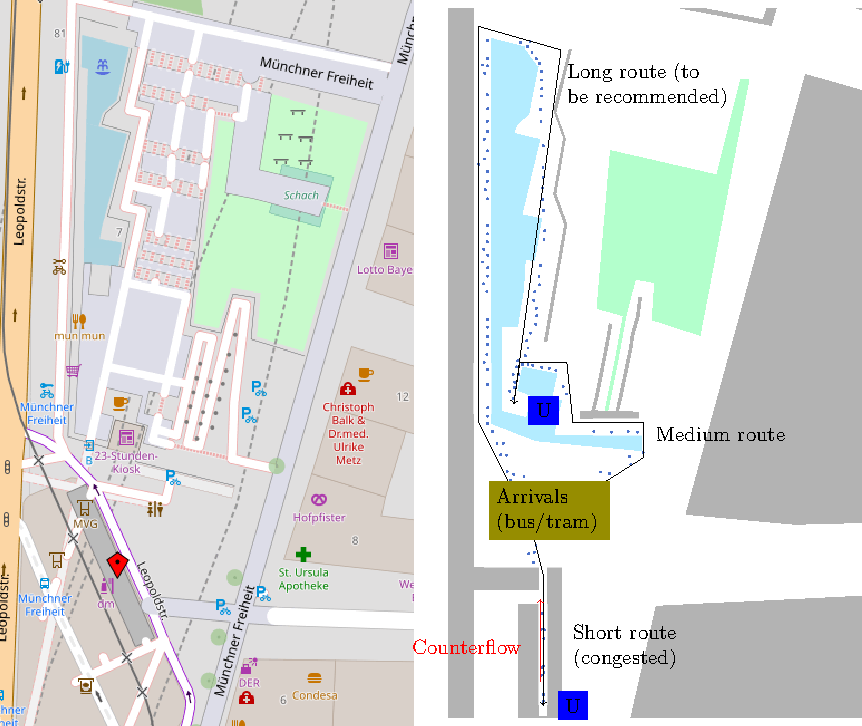
\includegraphics[width=0.73\textwidth]{../figures/investigation/RealisticScenario/applicationusecase.pdf} 
\caption[Real-life application scenario: rerouting pedestrians at the metro station Münchner Freiheit (Munich) ]{Real-life scenario: guiding football at the metro station Münchner Freiheit (Munich, Germany). Left: Bird's-eye view of the surface level from © OpenStreetMap \url{openstreetmap.org/copyright}. Right: Topography model in the \textit{Vadere} GUI. Obstacles are displayed in grey. The blue and green areas in Open Street Maps (left) are not accessible and are, therefore, modeled as (colored) obstacles.}
\label{fig:reallifeusecase}
\end{figure}





\subsection{Crowd guidance system: concept, model and implementation}

Fig.~\ref{fig:zentralesSzenario} depicts my proposal for a crowd guidance system applied to the use case Münchner Freiheit.  

\begin{figure}[hbt!]
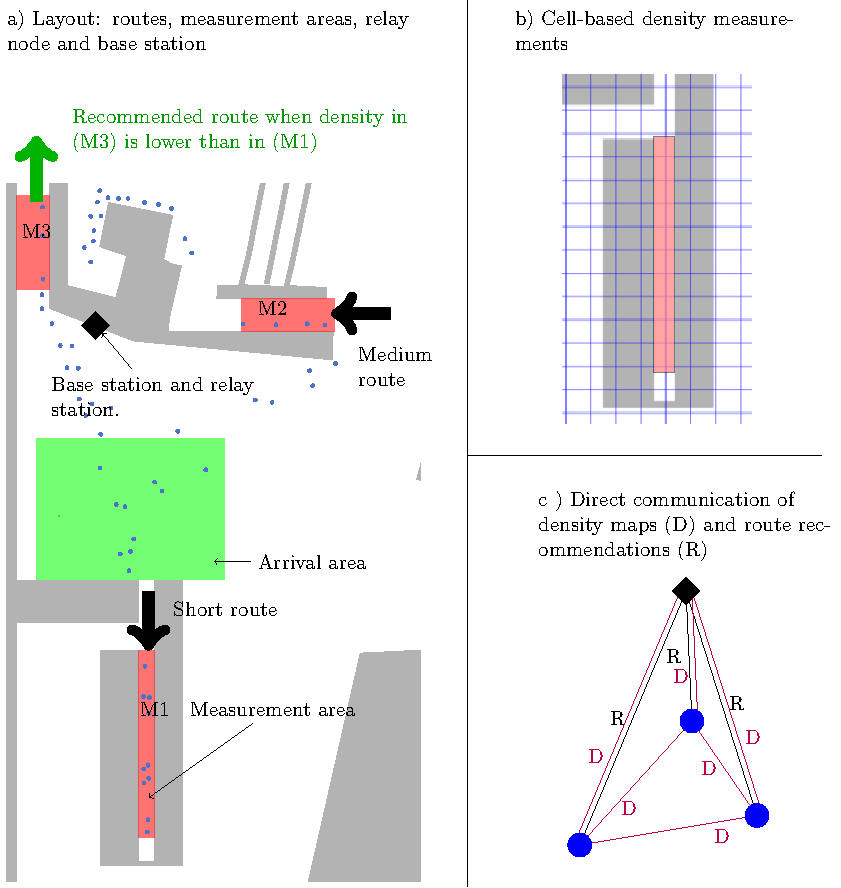
\includegraphics[width=0.82\textwidth]{../figures/investigation/RealisticScenario/conceptFinal.pdf} 
\caption[Proposed crowd guidance system with relay station]{Proposed crowd guidance system with controller station. Football fans (small blue dots) get off the bus or tram in the arrival area where an app provides route recommendations. The route recommendation algorithm, implemented in the controller station, compares the densities along the short (M1) and the long route (M3) every 2s (a). The long route is recommended if and only if the density in (M1) is higher than in (M3). The density values are average values derived from the density map application that counts pedestrian for each cell (b). Density information and route recommendations are disseminated in separate mobile apps using LTE sidelink communication (c) in the controlled mode.}
\label{fig:zentralesSzenario}
\end{figure}

%\subsubsection{Setup and components of the proposed crowd guidance system }
The components of the crowd guidance system, depicted in Fig.~\ref{fig:zentralesSzenario}, fulfill the following functions. The controller station, that is a computer including a network interface card for sidelink communication, evaluates the density-based route recommendation algorithm each time a fixed time interval has elapsed and disseminates the route recommendation over a mobile application in the crowd. 
The centralized computation of the  recommendation ensures that pedestrians do not have contradictory recommendations displayed on their apps.
The algorithm uses density measurements provided by the decentralized pedestrian density map application as input. For an overview of the data flow between apps and the route recommendation algorithm, see again Fig.~\ref{fig:regelkreisapplied} in Section~\ref{sec:crownet}.
Both apps, the route recommendation application and the pedestrian density map application, use LTE sidelink communication in the controlled mode. To prevent individuals from detouring, route recommendations are only displayed in the arrival area (25\,m$\times$15\,m) where football fans leave the bus or tram. The controller station is placed next to the arrival area to ensure coverage in the area where pedestrians arrive and need redirection information.

To test the concept through simulations, a system model is composed and implemented in \textit{CrowNet}, see Tab.~\ref{tab:composedrealistic}. The explicit method described in Section~\ref{sec:explicite} is used as update scheme. 

\begin{table}[hbt!]
\begin{footnotesize}
\begin{tabular}{p{1.4cm}p{3.6cm}p{3.5cm}p{4cm}}
\hline
Component & Sub-component & Model  & Implementation (Simulator) \\ \hline
Crowd  & Locomotion model & Optimal Steps Model & OptimalStepsModel (Vadere) \\
& Perception model &  Route choice probabilities & MultiPerceptionModel (Vadere)  \\
& Cognition model & Probabilistic Cognition Model & ProbabilisticCognitionModel (Vadere)  \\

Controller &
Time stepping alg. & Fixed interval (2s) & FixedTimeStepper (flowcontrol)  \\
&  Algorithm & Simple density algorighm & AvoidShort (flowcontrol) \\

Network & Application layer & Detour application &  CrownetUdpApp  (CrowNet/app.) \\
&& Density map application &  DensityMapAppSimple  (CrowNet/app.) \\
&Transport layer & Udp  & Udp (inet) \\
&Internet layer & Ipv4  & Ipv4NetworkLayer (inet) \\
&Air interface (PDCP) &  3GPP TS 36.323 & LtePdcpRrc(Ue/Enb)D2D (simu5G) \\
&Radio link layer (RLC) & 3GPP TS 36.322 &  LteRlc (simu5G) \\
&Medium Access layer (MAC) & TS 36.321  &  LteMac(Ue/Enb)D2D (simu5G) \\
&Physical layer (PHY) &  3GPP TS 36.201, 3GPP TS 36.211,-213 &  LtePhy(Ue/Enb)D2D (simu5G) \\
&$\rightarrow$ Channel model & 3GPP TR 36.873 (Microcell) & LteRealisticChannelModel (simu5G) \\
\hline
\end{tabular} 
\end{footnotesize}
\caption[Composite model for the simulation of the real-life use case]{Composite model of the crowd guidance system. 
  %%  https://www.3gpp.org/dynareport?code=36-series.htm
}
\label{tab:composedrealistic}
\end{table}


The \textit{Vadere} simulator provides mobility data and crowd behavior models, \textit{OMNeT++} simulates the mobile network, and \textit{flowcontrol} provides the route recommendation algorithm.

\FloatBarrier


\subsubsection{Modeling the topography and the arrival process in \textit{Vadere}}
To model the topography  of the metro station Münchner Freiheit at the surface level I use bird's-eye views of the station that are publicly accessible via Open Street Maps. The topography spans an area of 164\,m $\times$ 215\,m. Areas, pedestrians cannot or should not step on, like buildings and major streets are modeled as obstacles. Agents are spawned in source A which is the area where football fans leave the bus or the tram, see~Fig.~\ref{fig:topomodel}.

According to the public transport provider of Munich, an average of 1200 people per hour change from bus or tram to the underground train at Münchner Freiheit before a football game. Between the arrivals of two trams or buses, the value might be lower, but shortly after the arrival of a tram, it is considerably higher. To capture the worst case I use 3600 ped/h (= 60 ped/min). In the simulation this flow is realized by spawning 2 agents every 2\,s in source A (x\,=\,66\,m, y\,=\,77\,m, 4.4\,m$\times$3.6\,m). A counterflow is formed by pedestrians walking from the underground to the bus. The counterflow is spawned in source B (x\,=\,69\,m, y\,=\,41\,m, 1.75\,m$\times$1.5\,m). Agents spawned in source B are assigned to target B, which represents a bus stop where people board the bus. To achieve a qualitatively similar flow situation as observed on site (see Appendix~\ref{sec:countstudy}), two agents are spawned every 3\,s. The controller station and the base station are positioned close to the arrival area (x\,=\,62\,m, y\,=\,95\,m) to ensure coverage.



\begin{figure}
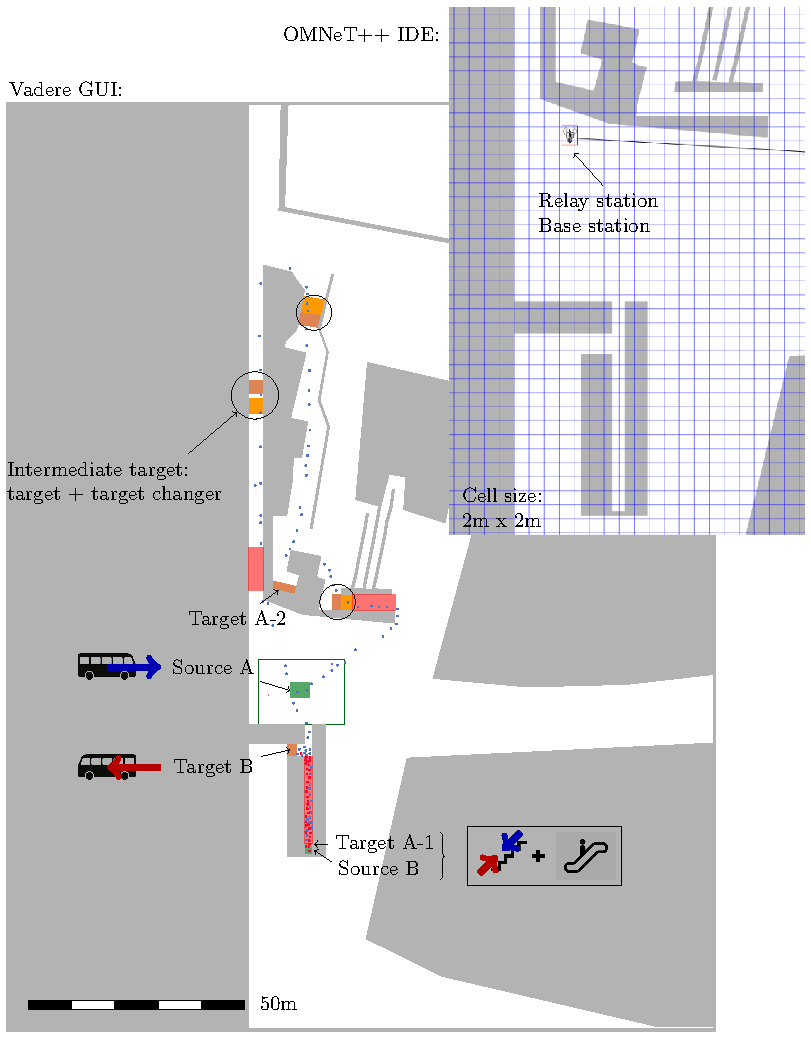
\includegraphics[width=0.95\textwidth]{../figures/investigation/RealisticScenario/topographymodel/topographymodel.pdf} 
\caption[Model of the topography]{Model of the topography (width: 164\,m, height: 215\,m). The topography and mobility behavior is modeled in the \textit{Vadere} simulator (GUI on the left) using sources (green), targets (orange) and target changers (yellow). Blue agents are spawned in source (A) and walk along the three routes to get to the train (targets A-1 and A-2). Red agents walk from the train (source B) to the bus (target B) and form a counterflow. Red areas are measurement areas. In the \textit{OMNeT++} simulator, the cell size, the position of the stationary relay station and the base station is defined.}
\label{fig:topomodel}
\end{figure}



\subsubsection{Route recommendation algorithm in \textit{flowcontrol}}

The density-based route recommendation algorithm computes a route recommendation every 2\,s, ensuring  the responsiveness of the crowd guidance system. A smaller time interval would not have an effect since the density measurements are updated every 2\,s. The basic idea of the algorithm is to recommend the long route if the density on the short route surpasses the density on the long route. This recommendation is then disseminated as mobile message. Otherwise, no route recommendation is sent. At each moment, the route recommendation is identical for all individuals, preventing group separations due to conflicting information. 
To make a decision, the route recommendation algorithm requires a density value for the routes. I expect the maximum density at the bottleneck of each route where the corridor width is the smallest. Therefore, measurement areas  are placed at the beginning of each route, see Fig.~\ref{fig:topomodel}. The dimensions and positions are listed in Tab.~\ref{tab:dimensioning}. Their identical area size ensures equal smoothing of the density over time. The pedestrians arrive in the measurement areas at about the same time because the distance to the arrival area is similar. Therefore the effect of a redirection is measured with a similar delay, and, the effect of delay on the route recommendation algorithm can be neglected.
\begin{table}[hbt!]
\begin{tabular}{llccc}
\hline 
Route &  Coordinates (x,y) in m   & Width in m & Height in m & Area in $\text{m}^2$ \\ 
& (Origin: bottom left corner) & & & \\ \hline
Short & (69.0,43.5) & 1.75 & 20.0 & 35.0 \\ 
Medium & (80.0,97.5) & 10.0 & 3.5 & 35.0 \\ 
Long & (56.0,102.0) & 3.5 & 10.0 & 35.0 \\ 
\hline 
\end{tabular} 
\caption[Dimensioning of the measurement ares]{Dimensioning of the measurement ares. The identical area avoids artificial density discrepancies.  }
\label{tab:dimensioning}
\end{table}

The \textit{SimpleDensityAlgorithm} is implemented in the \textit{flowcontrol} simulator. Every 2\,s, the algorithm receives a pedestrian density map from the controller station that is simulated in the mobile networks simulator \textit{OMNeT++}. The densities are mapped using the \textit{DensityMapper} provided by the \textit{flowcontrol} simulator.



\subsubsection{Mobile application for disseminating route recommendations in \textit{OMNeT++}}
Route recommendations are disseminated through a mobile application based on LTE sidelink. The controller station sends route recommendations to pedestrians in proximity. Received recommendations need not be forwarded  (single hop) because there are no obstacles  between the controller station and the arrival area. The single hop ensures that the network load is low. 

The mobile application is implemented as \textit{BroadcastControlApp} in the \textit{OMNeT++} module (Section~\ref{sec:omnet}). Every two seconds, the mobile application of the controller station can receive a route recommendation from the simulator \textit{flowcontrol}. The recommendation is sent as single packet via broadcast to  agents using UDP. 



%The propagation channel and protocol stack are captured by established models from the simu5G simulator, see Tab.~\ref{tab:composedrealistic}.





\subsubsection{Mobile application for measuring densities: density map application in \textit{OMNeT++}}
The route recommendation algorithm requires density measurements. For this purpose the density map application~\cite{schuhbaeck-2023-com} is employed (see again Section~\ref{sec:omnet}). In a real system the application would be implemented in the controller station. The application estimates the density for each cell based on the number of received beacons and based on density estimates shared by other devices. The parameter values can be found in Tab.~\ref{ref:densitymapparameters}.

The mobile application is composed of two services: One for disseminating beacons and one for dissemination density information (see again Section~\ref{sec:omnet}). The services are implemented as separate applications in the \textit{OMNeT++} module: as \textit{DensityMapAppSimple} application and as \textit{BeaconDynamic} application.

\begin{table}[hbt!]
\begin{footnotesize}
\begin{tabular}{p{3.1cm}p{2.4cm}p{0.7cm}p{7cm}}
\hline
Application  & Parameter & Value & Comment\\
\hline
DensityMapAppSimple &generationInterval & 2\,s & controls how often densities are updated\\
&mapTypeLog&  & Algorithm "Youngest measurement plus distance": Consideration of the actuality of the density value and the distance between the cell and the position of the device providing an estimate for the corresponding cell\\ 
&cellAgeTTL& 15\,s& exclude measurements/estimates older 15\,s \\
&alpha& 0.9 & Parameters of the aggregation algorithm: weight the normalized actuality with the factor 0.9 and the normalized distance with 0.1. 
\\
&stepDist& 60\,m & The distance between the cell and the position of the device providing a density estimate for the respective cell has no influence on the aggregation of the density values if it is below the stepDist\,=\,60\,m; assumption: if the cell is close enough \mbox{$<$\,60\,m}, density estimates are similarly accurate.  \\
&cell size & 2\,m& controls the spatial discretization  \\
BeaconDynamic & generationInterval & 0.5\,s & controls how often beacons are sent\\
 & maxAge & 5\,s & exclude beacons older 5\,s\\
\hline
\end{tabular}
\end{footnotesize}
\caption[Configuration of the density map application]{Parameter specifications for the density map application and the beacon application. I use default values except for the cell size that I reduce from 5\,m (default) to 2\,m since the smallest corridor width is 2\,m in the scenario.}
\label{ref:densitymapparameters}
\end{table}


\subsubsection{Modeling the protocol stack for LTE sidelink communication in \textit{OMNeT++}}


The LTE protocol stack is modeled as four layers: the Packet Data Convergence Protocol (PDCP) layer, the Radio Link Control (RLC) layer, the Medium Access Control (MAC) layer and the physical (PHY) layer, see again Fig.~\ref{fig:protocollstack} in Section~\ref{sec:modelcom}.


%The basic idea of the Packet Data Convergence Protocol (PDCP) is to cipher packets with an encryption key that can only be decrypted by the intended recipient and to assign each packet a sequence number for its identification. 


Different modes exist for the Radio Link Control (RLC) Protocol. I choose the unacknowledged mode which is recommended for direct communication~\cite{nardini-2018-com}. Data packets are segmented, sorted and assembled. Data received more than once is discarded. 


At the Medium Access Layer (MAC), the scheduling of resources is managed: every 1\,ms resources are distributed over 25 bands at a carrier frequency of 2.6\,GHz. 


At the physical (PHY) layer, the signal propagation and interference is modeled. As channel model I choose the standardized microcell LTE 3D channel model provided by the 3GPP. The channel model computes the power of a received signal which is then used to estimate the signal to noise interference ratio. This values is used together with Block Error Rate (BLER) curves to decide whether data is successfully received or not. 

The protocols and models of the four layers including the Packet Data Convergence Protocol (PDCP) layer are provided by the \textit{simu5G} framework, see the technical specifications (`TS') in Tab.~\ref{tab:composedrealistic}.


To enable direct communication in the simulation, the respective network interface card (NIC) in the mobile networks simulator's config file (*.ini) is selected: \textit{LteNicUeD2D}. To model the Adaptive Modulation and Coding (AMC) scheme, the \textit{amcMode} is set to "D2D" (device-to-device).
For the communication over broadcast, the internet layer is specified as follows: all agents are assigned to a multicast group that is addressed using the IPv4 protocol and a suitable network mask. 


\subsubsection{Modeling participation: proportion of people using apps in \textit{OMNeT++}}
In reality, only a part of the crowd would use the two mobile applications described before. Based on the findings from \cite{fonseca-2021-cdyn}, I choose a value of 40\% which reflects the regular usage of navigation applications for individuals which, I think, can be transferred to a crowd guidance system. I do not model pedestrians' awareness, but assume that whoever installed the route recommendation application perceives the recommendation through a notification. Accordingly, 40\,\% of the individuals are equipped with smart phones in the mobile networks simulation.



\subsubsection{Modeling crowd behavior in \textit{Vadere}}
The crowd model is composed of the locomotion model and the route choice model. For the locomotion behavior I use the Optimal Steps Model. To model how pedestrians distribute over the three routes when no guidance is provided, I use a discrete probability distribution that I derive from the survey data (Section~\ref{sec:reaction}). Agents spawned at source A are assigned to the three routes using a so-called target changer that is placed at source A in the topography model.
Route changes after receiving route recommendations are modeled in the \textit{ProbabilisticCognitionModel} which also uses probabilities values from the survey data. 

In the survey, participants were asked to rate the attractiveness of the three routes on a 5-point scale (1-5).
To estimate the route probabilities from the survey data, a model is needed that translates the Likert scaled route attractiveness into route probabilities.
I suggest a simple model to interpret the scores from the survey as route frequencies. I published the model in~\cite{mayr-2023-cdyn}. The idea of the model is that a survey participant who rated the shortest route at $4$, the medium route at $3$, and the long route at $3$ would pick the shortest route 4 out of $10 (=4+3+3)$ times, the medium $3$ out of $10$ times and the short $3$ out of $10$ times. I argue that this portrays the likely behavior in the long run.
With this in mind, I define the individual route probability  $p_{j,m}$ that a participant~$m$ selects route~$j$ as
\begin{equation}
p_{j,m} = \frac{l_{j,m}}{\sum_j l_{j,m}}
\label{eq:individualRoute}
\end{equation}
where $l$ is the route attractiveness that I take from the survey. Note that the division through  $\sum_j l_{j,m}$ achieves that the sum of probabilities equals 1: $\sum_ j p_{j,m} = 1$. 
This normalization  solves the problem that participants might interpret the scale differently, e.g., the route distribution is $[1/3,1/3,1/3]$ no matter whether a participant rated the routes with $[2,2,2]$ or $[3,3,3]$.  
I argue that the average of the single behaviors is a good characterization of the behavior of the population as a whole. Therefore, I define the route probability $p_{j}$ for the whole population as
\begin{equation}
p_{j} = \frac{1}{m} \sum_m p_{j,m} 
\label{eq:populationRoute}
\end{equation}
With Eqs.~\eqref{eq:individualRoute} and \eqref{eq:populationRoute}, route choice probabilities are inferred from the survey data.  Tab.~\ref{tab:routechoiceestimates} lists the estimated route probabilities for the group of footballs fans from the online survey (Section~\ref{sec:reaction}) with and without guidance. For the case with guidance, the route probabilities are computed for each message design separately because the survey showed that the message design has an effect.



 
\begin{table}[ht!]
\begin{footnotesize}

\begin{tabular}{lccc}
  \hline
  & \multicolumn{3}{c}{Route probabilities}\\ \cline{2-4}
Message design &$p_1$ (short) & $p_2$ (medium) & $p_3$ (long) \\ 
  \hline
     Arrow & 35 & 31 & 33 \\ 
    Arrow + top down view & 34 & 31 & 35 \\
    Arrow + team spirit  & 36 & 29 & 35 \\ 
    Arrow + top down view + team spirit & 32 & 30 & 38 \\
  Congestion info + arrow & 29 & 36 & 35 \\ 
 Congestion info + arrow + top down view & 27 & 35 & 38 \\
 Congestion info + arrow + top down view + team spirit & 27 & 34 & 38 \\ 
   \textbf{Congestion info + arrow + team spirit} \textit{(parameters} &\textbf{25} & \textbf{35} & \textbf{40} \\ 
 \textit{of the cognition model)} &&& \\    
 \cline{1-4}
     Prior to information \textit{(parameters of the target changer)} & 49 & 30 & 22 \\  

\hline
\end{tabular}
\end{footnotesize}
\caption[Route probabilities forfor the survey data]{Route probabilities for the football fans. The route probabilities were estimated from survey data (Section~\ref{sec:reaction}) using the proposed model: Eqs.~\eqref{eq:individualRoute} and \eqref{eq:populationRoute}. The idea of the model is to translate the Likert scores by which survey participants rated the attractiveness of a route 
into percentages of passengers $p_i$ that would take that route. The most convincing design is the one with the lowest probability of taking the congested short route (bold).  }
\label{tab:routechoiceestimates}
\end{table}



Without route recommendations, the short route is chosen with a probability of 49\,\%. This value deviates from the probability estimate from a manual counting experiment that is between $0.75 ... 0.82$ (see Appendix~\ref{sec:countstudy}). I attribute this large difference to the coarse nature of the counting study and to the assumption of a steady flow. Also, there were uncontrollable factors such as age and gender. The route choice probabilities in Tab.~\ref{tab:routechoiceestimates} indicate that with the
 message design \textit{Congestion info + arrow + team spirit} more pedestrians are willing to take a detour than with the other message designs because the route probability of the short route is the lowest. Therefore, I use this message design in my investigations. The associated route probabilities serve as parameters of the \textit{ProbabilisticCognitionModel}. The route choice probabilities corresponding to the case without route recommendation serve as parameters for the target changer.



\FloatBarrier
\subsection{Design of the simulation study}

To assess whether safety and comfort can be improved with a crowd guidance system, I run simulations of the scenario with and without crowd guidance system. Due to the long duration of a single simulation run (see Section~\ref{sec:performanceevaluation}), I refrain from repetitions.
I argue that the measurement areas are large enough ($35\,\text{m}^2$) to smooth out stochastic effects so that running the simulation with different seeds would not change the qualitative behavior that I am interested in.


\subsubsection{Key performance indicators}
I choose Fruin's Level of Service~\cite{fruin-1971-cdyn} and the Pedestrian Comfort Level~\cite{tfl-2019-cdyn} (see Section~\ref{sec:fundamentaldiagram}) as key performance indicators. The density $d$ is measured every 0.4\,s in each measurement area (M1, M2, M3) by dividing the number of agents $N$ by the area size $A$ (classical method): $d = N / A$.
To evaluate the Pedestrian Comfort Level~\cite{tfl-2019-cdyn}, the specific flow is derived from the measured densities according to the Kladec formula, see Eq.~\eqref{eq:kladec}. Therefore, flow and density are averaged values. The large size of the measurement area smooths out stochastic differences between different simulation runs (seeds). 
In addition, the number of lost packets, the packet life time, the number of generated route recommendations, the density measurements provided by the density map application, and the ratio of simulation time and real time are measured, see Tab.~\ref{tab:measurementquants}. Importantly, I expect the true density to be underestimated since only 40\,\% of the agents use the density map application in the scenario. 

\begin{table}[hbt!]
%\begin{footnotesize}
\begin{tabular}{|p{4cm}|p{10cm}|}
\hline 
\textbf{Quantity} &  \textbf{Serves to evaluate ...} \\ \hline
Density (ground truth) & Fruin's Level of Service~\cite{fruin-1971-cdyn} (safety) and the Pedestrian Comfort Level~\cite{tfl-2019-cdyn} (comfort); measured every 0.4\,s. \\ \hline
Estimated density from app  & Suitability of the density map application for providing density data. Measured every 2\,s. \\ \hline
Number of route recommendations  & Verification of the route recommendation algorithm. I expect that, due to the counter-flow, the long route is continuously recommended. Measured every 2\,s. \\ \hline
Ratio of simulation time and real time, RAM usage, CPU usage  & Real-time capability of the simulation setup. \\  \hline
Number of lost packets, packet lifetime  & Reliability of the information provision through direct communication. \\ \hline 
Total number of agents & Separation of inflow phase and steady flow. \\ \hline 
\end{tabular} 
%\end{footnotesize}
\caption{Overview of key performance indicators and quantities of interest. Several quantities of interest are measured to evaluate the performance and reliability of the proposed crowd guidance system. Also, the computational effort is monitored: the RAM and CPU usage of the three Docker containers (\textit{OMNeT++, flowcontrol, Vadere}).}
\label{tab:measurementquants}
\end{table}



\subsubsection{Inflow and steady state flow}
Two system states are to be assessed within one simulation run: the inflow and a steady state flow. One can expect that the inflow takes the first 220\,s, that is the time an agent with average speed (1.34\,m/s) needs to pass the longest route (300\,m). After, the flow settles into a steady state. To observe both states, I choose a simulation duration of 10\,min (600\,s).  





\subsection{Proof of concept through simulations}
In this sub-section I present the results of the simulation study. I check whether expectations regarding the system behavior are met and look at the key performance to evaluate how the crowd guidance system affects the traffic situation.


\subsubsection{Dynamic change: inflow and steady-state flow}

Fig.~\ref{fig:realistisceNumberofPeds} depicts the total number of agents over time. As expected, the number of agents increases until 220\,s which indicates the inflow state. At around 220\,s, the number of agents stagnates, thus, a steady state flow is reached. The maximum number of agents is 136 agents in the setting with guidance. Therefore, a maximum of 54 agents (40\,\%) communicate over the mobile network at the same time. In the three measurement areas the steady state is reached even earlier because they are located at the beginning of the routes. It is reached after 120\,s at the short route, see~Fig.~\ref{fig:densitiesrealisticusecase}~(top). On the medium and long route, the density keeps oscillating beyond 50\,s due to the low number of agents. 

\begin{figure}[hbt!]
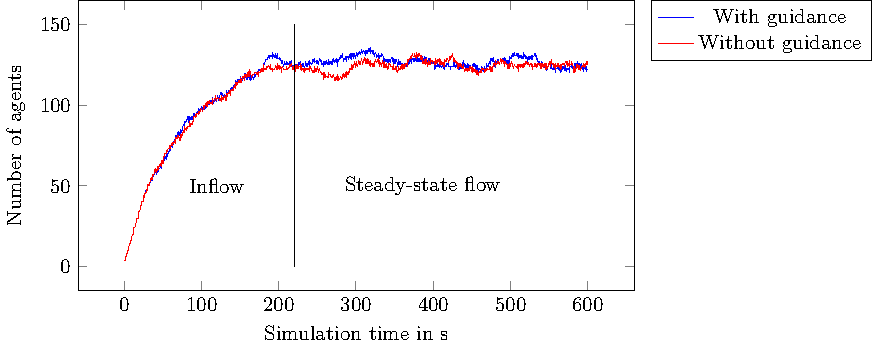
\includegraphics[scale=1]{./investigation/RealisticScenario/comparison/numberofpeds.pdf} 
\caption[Number of agents over time]{Total number of agents in the topography over time. After 220\,s, the number of agents does not change which indicates a steady state flow. The maximum number of agents is 133 (no guidance) and 136 agents (with guidance).}
\label{fig:realistisceNumberofPeds}
\end{figure}




\subsubsection{The crowd guidance system improves the level of service and safety}
%I use the maximum densities of each route to evaluate football fans' safety during transfer. 
Fig.~\ref{fig:densitiesrealisticusecase} depicts the density without and with crowd guidance for each route. The densities on the short route are always higher than on the medium and long route.  At the longer routes, a level of service A is achieved regardless of whether crowd guidance is present or not: In reality pedestrians would walk with their desired speeds.
For the short route, a level of service E persists for most of the time indicating that the crowd movement temporarily stops and passing maneuvers are impossible. This constitutes a safety risk. With guidance, the better level D is achieved most of the time with less restricted movement which allows some pedestrians to pass each other. Note that this is the best achievable level in the scenario due to the counter flow of 70\,ped/m/min, which corresponds to a level D all by itself. Therefore, I conclude that the proposed guidance system improves the service quality and safety. 

\subsubsection{Redirecting only a few agents resolves congestion on the critical route}

Redirecting only a few pedestrians has a large effect on the congestion situation. With guidance the density on the short route is \textrm{$0.3\,\text{ped/m}^2$} lower than without guidance, see time slots (1)-(3) in Fig.~\ref{fig:densitiesrealisticusecase}. According to the Kladec Eq.~\eqref{eq:kladec} at least 24\,ped/min needed to be redirected to achieve such a decrease of the density.

The simulation, on the other hand, demonstrates that it suffices to redirect only 6\,ped/min. This can be explained by the change in the dynamics of the movement behavior as a result of the redirection: The redirection prevents the opposing flows from blocking each other. Fig.~\ref{fig:snapshotsrealisticusecase} depicts how congestion evolves for the system without guidance and how congestion is resolved for the system with guidance. 


\begin{figure}[H]
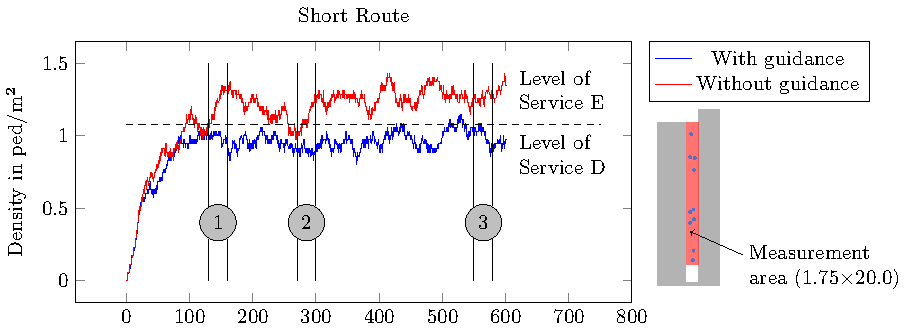
\includegraphics[width=14.8cm]{./investigation/RealisticScenario/comparison/densitiesovertimeRealisticSce-1.pdf} 
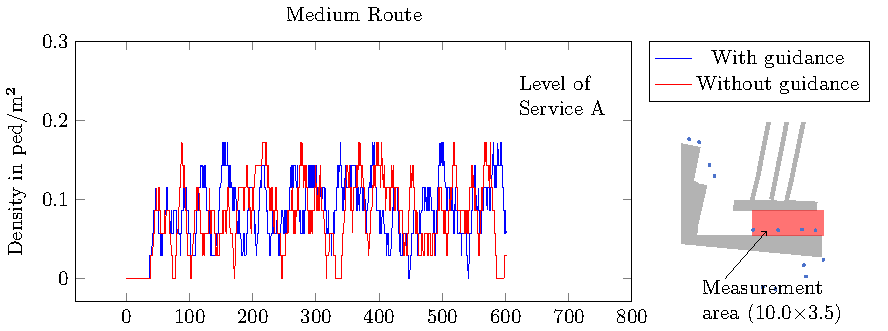
\includegraphics[width=14.4cm]{./investigation/RealisticScenario/comparison/densitiesovertimeRealisticSce-2.pdf} 
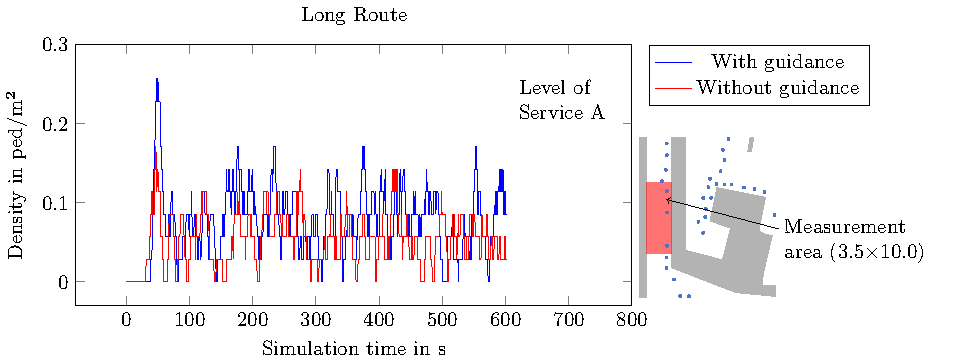
\includegraphics[width=15.6cm]{./investigation/RealisticScenario/comparison/densitiesovertimeRealisticSce-3.pdf} 
\caption[Densities for safety evaluation]{Densities for safety evaluation with and without guidance. Providing route recommendations reduces the density on the short route (top): most of the time a  level of service D can be achieved. Congestion is prevented only in the setting with guidance: the density does not increase within the time slots (1),(2),(3). Fig~\ref{fig:snapshotsrealisticusecase} depicts the congestion situation for time slot (1). }
\label{fig:densitiesrealisticusecase}
\end{figure}



\begin{figure}[H]
\includegraphics[width=0.94\textwidth]{./investigation/RealisticScenario/snapshots_.pdf} 
\caption[Resolving congestion through redirecting pedestrians]{Resolving congestion through redirecting pedestrians.
Without guidance, the short route is congested due to the counter-flow: several agents wait in front of the route entrance (see top row). With guidance, the route is less congested (bottom row).  Route recommendations are only displayed within the arrival area. Informed agents are marked with a circle: 40\,\% of them take the recommended long route, 35\,\% take the medium and 25\,\% take the short route.}
\label{fig:snapshotsrealisticusecase}
\end{figure}


%Without guidance, the short route is congested: several agents wait in front of the route entrance. The congestion forms within 30s (see density increase in time slot (1) in Fig.~\ref{fig:densitiesrealisticusecase}) and then dissipates again (see density decrease in the area between 1 and 2). The crowd guidance system prevents congestion: the density is almost fixed in time slot (1), although the initial conditions for the system with and without guidance are similar, see intersection of the curves at the beginning of time slot (1) in Fig.~\ref{fig:densitiesrealisticusecase} (top). Moreover, the crowd guidance system is capable of repeatedly preventing or resolving congestion situations, see time slots (1-3).







\subsubsection{No improvement of comfort due to the counter-flow}

%No improvement of perceived comfort.
To evaluate comfort, the Pedestrian Comfort Level is analyzed. Converting the densities into flows using Eq.~\eqref{eq:kladec}, the flow values are far higher than the recommended threshold of 17\,ped/m/min considered as comfortable for such scenarios, see Fig.~\ref{fig:comfort}.  Note, that the threshold value does not take into account that soccer fans, who share a social identity, may perceive proximity and congestion as less uncomfortable than individuals. Nevertheless, the threshold value is exceeded by a factor of four and I expect them to feel uncomfortable. I conclude that the pedestrian guidance system, while it improves safety, does not suffice to ensure travel comfort.

\begin{figure}[H]
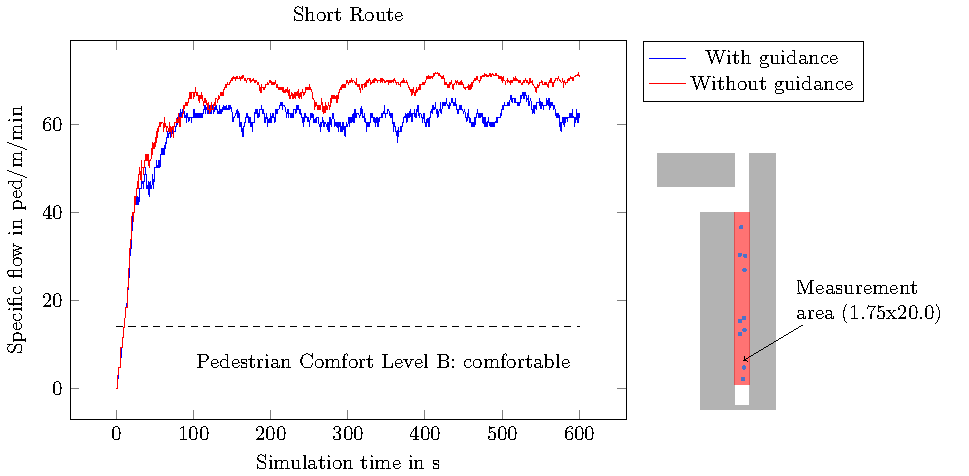
\includegraphics[width=\textwidth]{./investigation/RealisticScenario/comparison/flowovertimeRealisticSce.pdf} 
\caption[Specific flows at the short route] {Specific flows at the short route for comfort evaluation. The flows are derived from the density measurements using Eq.~\eqref{eq:kladec}. Due to the counterflow, the pedestrian comfort level B is never reached. }
\label{fig:comfort}
\end{figure}







\subsubsection{Verification of the route recommendation algorithm}
Fig.~\ref{fig:numberRecommRealistic} shows the number of route recommendations over time.
As expected, the route recommendation algorithm recommends the long route every 2\,s once the route recommendation is active because the density on the short route is always higher than on the long route, that is, the route recommendation algorithm works correctly.

\begin{figure}[H]
\centering
\begin{tikzpicture}
\node[] at (0,0) {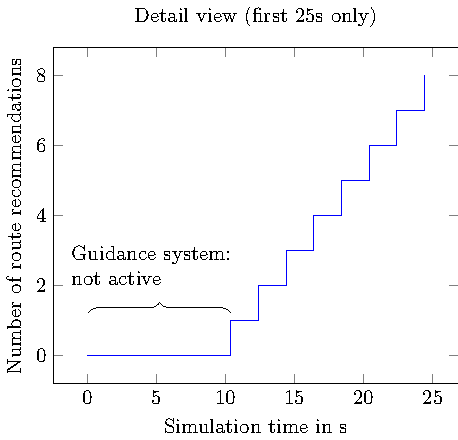
\includegraphics[width=7cm]{./investigation/RealisticScenario/comparison/numberRecommRealisticScenario-1.pdf} };
\node[] at (7.5,-0.0) {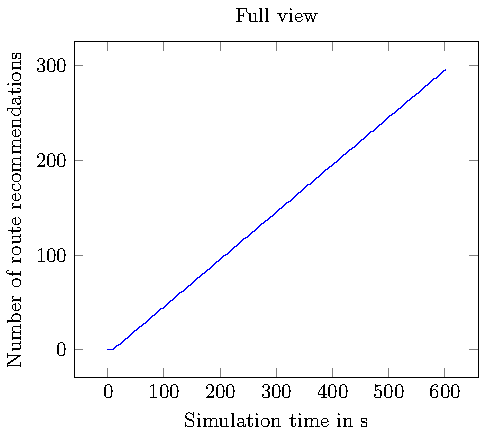
\includegraphics[width=7.2cm]{./investigation/RealisticScenario/comparison/numberRecommRealisticScenario.pdf} };
\end{tikzpicture}
\caption[Number of route recommendations]{Number of route recommendations. During the first 10\,s, the guidance system is not active (left). As soon as it starts working, the route recommendation algorithm continuously and correctly recommends the long route due to congestion along the short route (right). }
\label{fig:numberRecommRealistic}
\end{figure}

\subsubsection{The density map application provides suitable density measurements}


In the following, it is evaluated how suitable the decentralized density map application~\cite{schuhbaeck-2023-com} is for providing density measurements. Since the route recommendation is computed in the controller station, one needs to look at the density values of the application of the controller station. As expected, the density is underestimated because only 40\,\% of the agents share their location, see Fig.~\ref{fig:densityerrordef}. 

The scaled densities, that are, the densities that would be achieved if 100\,\% of the agents shared their location, are similar to the ground truth: compare the green and black curves in Fig.~\ref{fig:densityerrordef}. Therefore, relative density differences between routes are measured correctly given that position-sharing agents are evenly distributed over routes. This is promising for future applications, though it would be desirable to capture absolute values more accurately. 


Since density differences, not absolute values, drive the algorithm I conclude that the density map application is suitable as data provider for the suggested density-based route recommendation algorithm.


 

\begin{figure}[H]
\centering
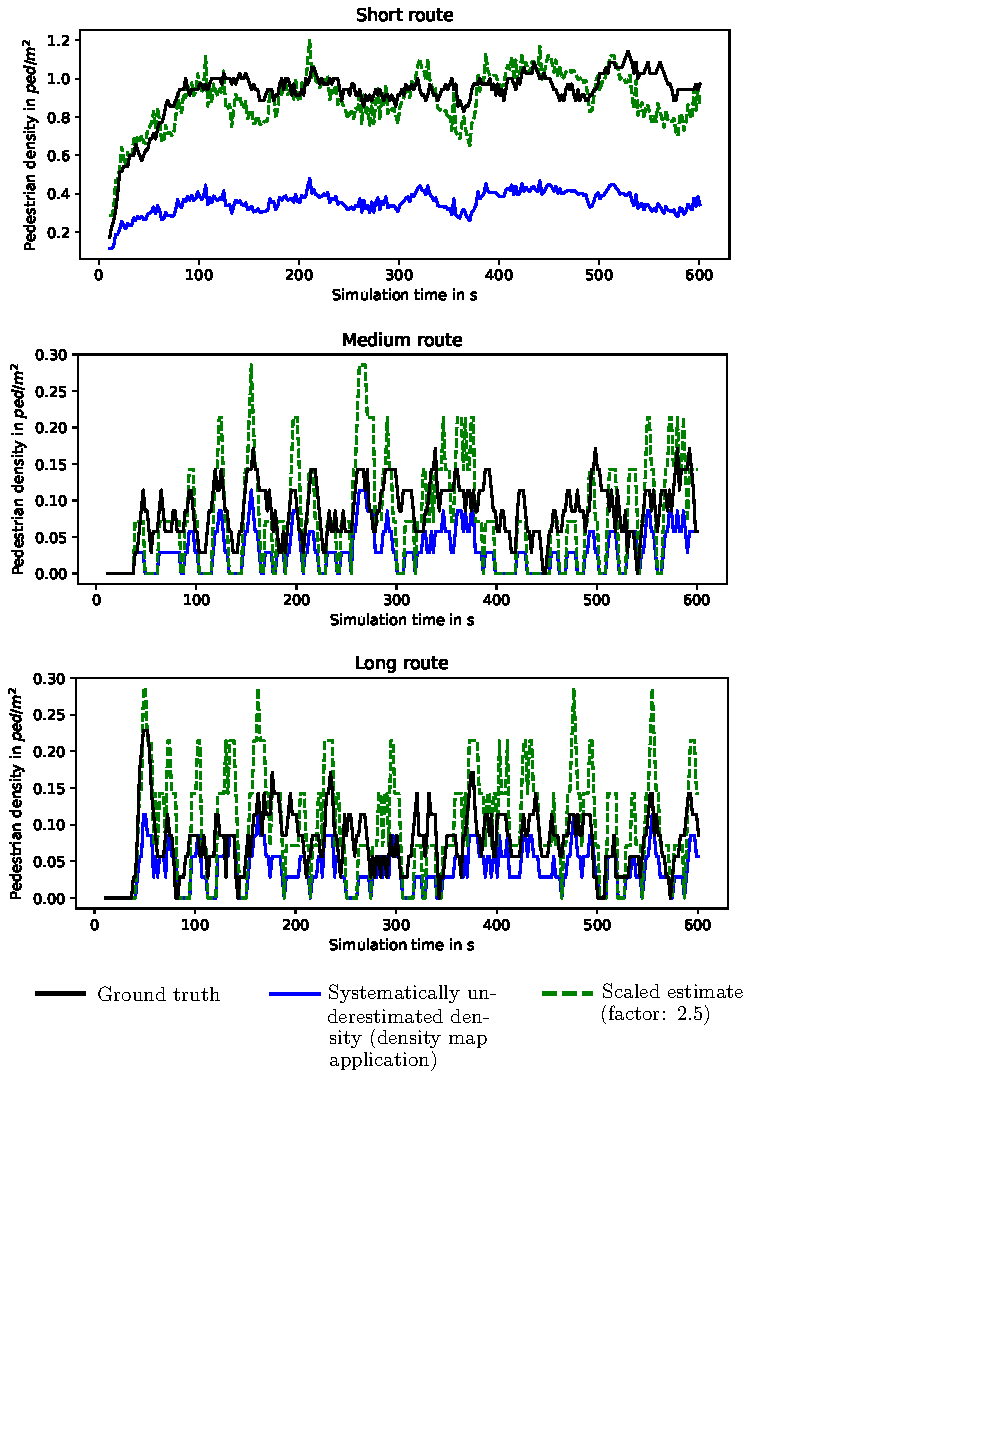
\includegraphics[width=0.86\textwidth,trim={0cm 6cm 4cm 0cm},clip]{../figures/investigation/RealisticScenario/densityestimates/densityestimates2.pdf} 
\caption[Density estimates from the decentralized density map application]{Density estimates from the decentralized density map application (setting with guidance).  The blue curve corresponds to the density estimates derived at the controller station. Since only 40\,\% of the agents share their position and density data, the density is systematically underestimated. The green curve is the same as the blue curve but scaled with a factor 2.5 which represents the case that 100\,\% of the agents would share their position. }
\label{fig:densityerrordef}
\end{figure}

\newpage


\subsubsection{The time between two route recommendations suffices to disseminate information and density data}

The chosen value of 2\,s for the route recommendation interval requires that information is transmitted in less than 2\,s. Otherwise, decisions would be based on outdated data. Therefore it is necessary to look at the duration of the information dissemination. I use the packet lifetime, that is, the time a packet travels from its sender to a receiver over the mobile network. The maximum lifetime of a packet disseminated over the route recommendation application is 27\,ms, see Tab.~\ref{tab:packetlifetimerealisticscen}. There is no packet loss because all of the 13995 packets are received successfully. As the maximum packet lifetime is much smaller than 2\,s, I conclude that route recommendations are always received in time. 
To ensure the the received density information is not obsolete, I look at the packet lifetime and the packet loss of the density map application. The packet loss is 50\,\% (only 861,419 of 1,751,011 packets arrive) which is high given that only 54 people communicate at the same time.
Nevertheless, the maximum packet lifetime is only 203\,ms which is again smaller than 2\,s. Since both application provide information in less than 2\,s, I conclude, that the chosen two seconds interval is suitable. 

\begin{table}[hbt!]
\centering
Packet lifetime in seconds \\
\vspace{0.1cm}
\begin{tabular}{|l|l|l|l|l|}
\hline 
Application &  mean & std & min & max \\
\hline 
Route recommendation application & 0.021 & 0.001 & 0.011 & 0.028 \\ \hline
Density map application  & 0.026 & 0.008 & 0.016 & 0.265  \\
\hline 
\end{tabular}
\caption[Packet lifetimes]{Packet lifetimes. The controller station sends route recommendations over the route recommendation application to agents. Agents and the controller station share density measurements over the density map application. In total, 13,529 packets lifetimes are collected for the route recommendation app, and 861,419 for the density map application from which the above statistics are derived. }
\label{tab:packetlifetimerealisticscen}
\end{table}







\subsection{Performance evaluation}
\label{sec:performanceevaluation}
The performance evaluation is based on the simulation runs executed on a virtual machine with 80 CPUs and 94GB RAM, see Appendix~\ref{sec:VirtualMachine}. One can observe that adding a crowd guidance system to a crowd simulation drastically increases the simulation effort, see Tab.~\ref{tab:runtimes}. With guidance, the simulation took approximately 184 times longer. The reason for this is the extensive mobile communication simulation, which becomes slower the more communication takes place. This can be seen from the increase in the ratio of simulation time to real time during the inflow phase where the number of agents increases, see Fig.~\ref{fig:performance}. 
After simulating 220\,s, the ratio of simulation time and real time varies strongly. The lower limit is approximately 25, which means that in the best case the simulation is only 25 times slower than real time. In the worst case, however, the ratio is 150. It is therefore not possible to simulate events in real time with the given hardware.

\begin{table}[hbt!]
\centering
\begin{tabular}{|p{3cm}|p{3.7cm}|p{1.3cm}|p{1.3cm}|p{1.9cm}|}
\hline 
Simulation & Simulators & Start & End & Duration\\ 
\hline
Crowd without guidance & \textit{Vadere} & 19:15:54 & 19:17:14 & 1.33 min \\ \hline
Crowd guidance system & \textit{Vadere, OMNeT++, flowcontro}l & 19:17:14 & 23:21:33 & 244.3 min \\
\hline 
\end{tabular} 
\caption[Simulation runtimes]{Simulation runtimes measured on 16 Dec 2023. The simulation of the crowd guidance system requires coupling the simulators \textit{Vadere, OMNeT++} and \textit{flowcontrol}. Due to the extensive mobile communication simulation, the simulation with a crowd guidance system based on direct communication takes 184 times ($=224.3/1.33$) longer than a crowd simulation without.}
\label{tab:runtimes}
\end{table}


Simulating  a guidance system also requires careful resource planning, as the RAM usage increases over the simulation time, see Fig.~\ref{fig:performance} (right). This makes the execution of simulation runs in parallel inefficient, as RAM must be reserved.


\begin{figure}[hbt!]
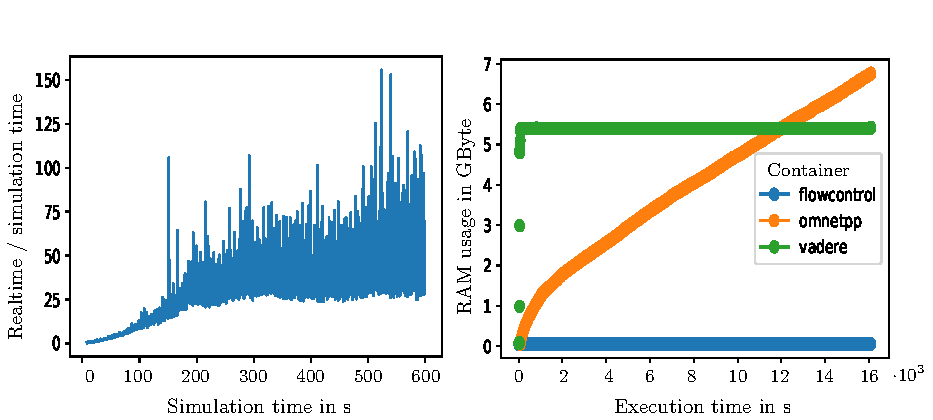
\includegraphics[width=\textwidth]{../figures/investigation/RealisticScenario/PerformanceEval/performanceeval.pdf} 
\caption[Performance of the simulation with crowd guidance]{Performance of the simulation with crowd guidance. The simulation is not real time capable: it is up to 150 times slower than the real time process (left). The RAM allocated by the mobile networks simulator \textit{OMNeT++} increases over time (right).}
\label{fig:performance}
\end{figure}

\subsection{Summary, model validation, limitations}

\subsubsection{Summary and lessons learned}

In this section, I proposed a complete crowd guidance system and simulated it to investigate whether it can improve the congestion situation in a real-life use case. 
First, I modeled the crowd guidance system by combining previously tested component models into an overall model: a density-based route recommendation algorithm, a crowd model and two mobile applications based on LTE sidelink communication. 
The first mobile application senses the crowd and the second disseminates route recommendations. 
The route recommendation algorithm is evaluated every two seconds and recommends the longest route among three routes if and only if the pedestrian density on the congested short route is higher than on the long route. 

To test the concept, a scenario before a football match at Münchner Freiheit metro station (Munich, Germany) was modeled where football fans change from the tram or bus to the underground which leads to congestion at the short route. The situation is aggravated by an anti-directional passenger flow. 
To find suitable parameters for the route choice model, route probabilities were estimated from survey data for which I suggested a novel model that converts the Likert-scaled survey data to route probabilities. 

A simulation study was conducted with and without the crowd guidance system. 
The results demonstrated that the crowd guidance system can improve the safety. Without the system the level of service has a level E and with the redirection it reaches a level D which allows pedestrians to pass each other and thus prevents congestion at a critical level. 
On the other hand, another key performance indicator, the pedestrian comfort level, did not improve considerably.

From an engineering perspective, it was demonstrated that the system fulfills functional requirements:
The results showed that the suggested time interval for the route recommendation algorithm of two seconds is feasible because the information is transmitted much faster over the mobile network. 


Importantly, not all people need to use the mobile applications. Partial usage leads to a systematic underestimation of the density. However, this does not have any effect on the route decision because the route recommendation algorithm relies on the density difference between routes. Crucially, it suffices to redirect relatively few people to resolve congestion in the real-life use case. Therefore, I conclude that the proposed crowd guidance system can indeed improve the traffic situation. 

\newpage

Based on these findings I answer my research question:



\begin{tcolorbox}[title=How can crowds be redirected through mobile applications based on direct communication technologies? (RQ)]
The crowd guidance system composed of the following components answers the question: Route recommendations are computed using a density-based algorithm. Densities are measured through a LTE sidelink-based mobile communication. The recommendations are disseminated in the crowd via another LTE sidelink-based mobile application.
\end{tcolorbox}


\subsubsection{Model validation}

The simulation model is made up of several sub-models that have already been validated against empirical data and simulation data, mainly the Optimal Steps Model for locomotion behavior and the 3GPP LTE channel model for mobile communication. The new route recommendation algorithm has a control function, but does not model a physical system. Thus, as an isolated component, it cannot be checked against measured data. The fact that the main component models have already been validated is a good prerequisite for the validity of the composed model. Nevertheless, the whole system can only be validated once empirical data is available that is when the system has been rolled out in reality. Thus, at this point, validation of the complete system must remain a task for the future.



\subsubsection{Limitations and future directions}



In the real-life use case, flows differed strongly between the possible routes. Therefore, small fluctuations of the densities had no effect on the route decision. If flows and densities of the routes are more similar, a smoothing procedure may be necessary. On the other hand, the use case is most interesting when a strong preference for one route causes congestion.

The density map application systematically underestimates the density if only a proportion of the virtual pedestrians used the measurement application which is a realistic assumption. In my scenario the underestimation had no effect on the decision of the route algorithm since the app users were evenly disseminated over the routes. If this is not the case, additional measurements and scaling procedures may be necessary. 

The parameters of the route choice model were estimated using a simple model that interprets Likert-scaled route attractivenesses from the survey as route frequencies in the long run. The uncertainty of the estimated route choice proportions was not part of the study. It would be interesting to analyze how the uncertainties of the route choice proportions affect the key performance indicators. 

Although the number of app users was low, the packet loss was high for the mobile application that measures densities using sidelinks. It would be interesting to analyze how scalable the mobile application is regarding the number of app users and how this affects the accuracy of the density estimates. Also, it would be interesting to test the system in the uncontrolled communication mode without base station.

The simulation of ten minutes real time took more than four hours due to the time-consuming mobile communication simulation. Consequently, parameter studies with many samples were infeasible. To accelerate the simulation, one could replace the mobile communication components by suitable surrogate models. 


\section{Summary of studies}



In this chapter I assessed how crowds can be guided through direct communication technologies. 
Firstly, the suitability of direct communication technology for disseminating detour information in a crowd was investigated using a scenario where obstacles impaired wave propagation (RQ-1). The study was split into two parts: Finding the minimum number of pedestrians in the scenario to overcome shadowing and assessing the  information dissemination in the absence of shadowing using forward propagation and global sensitivity analysis. The uncertain parameters `number of pedestrians', the `time interval' of the information broadcast, and the `transmitter power', that served as non-influential control parameter, were propagated to construct polynomial chaos expansions.  As expected, the control parameter had no influence. The results showed that the median of the packet lifetime depends only on the time interval of the broadcast. The crowd size slightly affected the minimum and maximum packet lifetimes. The time between two broadcasts was always more influential than the number of agents. The study strongly indicated that, despite interference, detour information was always provided within 10\,s. This is sufficiently fast enough to inform a crowd.


Secondly, I investigated the suitability of route recommendation algorithms (RQ-2). Since state-of-the-art algorithms were unsuitable, I proposed three heuristics: One that recommends routes sequentially, one that recommends the route with the lowest density, and an even simpler algorithm that always recommends the longest route among the available routes if the direct short route experienced higher densities. 
The algorithms were compared in a simulation study for an unknown level of compliance varied between 0\,\% and 100\,\%. The two density based algorithms resolved congestion at lower compliance rates than the sequential procedure. Interestingly the maximum densities did not differ statistically and all algorithms successfully resolved congestion. However, fewer redirection measures were necessary with the simplest algorithm that provides redirection measures if and only if the short route is more congested than the long route.  


Thirdly, I investigated the effect of message design on compliance behavior (RQ-3). 
I developed eight message designs and tested them on over 1400 test subjects in an online survey that was based on a real-life scenario  at the metro station Münchner Freiheit (Germany, Munich). The survey was conducted with two groups: Football fans for which I assumed a shared social identity and a control group of mainly students.
The findings indicated that people are willing, in principle, to follow route recommendations provided by an app. However, there was no ideal message design that best fulfilled that task to change their behavior independently of the social group. Messages that appeal to the team spirit of football fans increased their compliance when combined with other message components, but had no effect on students and faculty associates where social identification was lower. Providing real-time information on congestion proved most effective in fostering compliance.

%
Finally I answered my research question of how crowds can be redirected using direct communication technology. I proposed a crowd guidance system, applied it to the real-life use case Münchner Freiheit, and tested it in a simulation study.
The crowd guidance system is composed of a density-based route recommendation algorithm, the crowd model and two mobile applications based on LTE sidelink communication, one for sensing and another one for redirecting the crowd. To find suitable parameters for the route choice model, I estimated route probabilities from the survey data.  
The simulation study demonstrated that the crowd guidance system can lift the service level from E to D. At the same time comfort remained at a low level. 
The results also showed that the suggested time interval of two seconds between two evaluations of the route recommendation algorithm is feasible because information is transmitted much faster over the mobile network. 
Importantly, I could show that if only a proportion of the people uses the sensing application the underestimated densities have no negative effect because the route recommendation algorithm relies on density differences between routes. Crucially, I found that redirecting only relatively few people suffices to resolve congestion.
On the whole, I conclude that my crowd guidance system can indeed improve the traffic situation.
